\documentclass[11pt]{article}
\usepackage[utf8]{inputenc}
\usepackage{amsmath}
\usepackage{natbib}
\usepackage{graphicx}
%\usepackage[spanish, es-minimal]{babel}
\usepackage[spanish, es-minimal, english]{babel}
%\usepackage[vmargin=0.8in, hmargin=1.00in]{geometry}
\usepackage[vmargin=0.7in, hmargin=1.0in]{geometry}
\usepackage{lipsum}
\usepackage{longtable}
\usepackage{pdfpages}
\usepackage{listings}
\usepackage{hyperref}
\usepackage{url}

\newcommand\U[1]{\ensuremath{\mathrm{#1}}}
\newcommand\K{\U{K}}
\newcommand\cm{\U{cm}}
\newcommand\AU{\U{AU}}
\newcommand\g{\U{g}}
\newcommand\msolagno{M_\odot\,\U{yr^{-1}}}

\newcommand\acre{\ensuremath{_{\mathrm{acre}}}}
\newcommand\eff{\ensuremath{_{\mathrm{eff}}}}
\newcommand\Int{\ensuremath{_{\mathrm{Int}}}}
\newcommand\Ext{\ensuremath{_{\mathrm{Ext}}}}

\newcommand\BowshockFig[1]{
  \includegraphics[width=\figwidth, clip, trim=10 10 10 10]
  {#1}
}
\newcommand\raiselabel[1]{\raisebox{0.9\figwidth}[-0.5\figwidth]{#1}}
\newcommand\raiselabelPho[1]{\raisebox{0.62\figwidth}[-0.5\figwidth]{#1}}



\title{SMC planetary nebulae in S-PLUS }

%\author{
   %Bolsista: Luis Angel Gutiérrez Soto\\
   %Coordenadora: Claudia Lucia Mendes de Oliveira 
%}
\date{}

\begin{document}
\maketitle

\section{Science verification}
\label{sec:ini}

\begin{figure}
\centering
\begin{tabular}{l l}
  \includegraphics[width=0.5\linewidth, trim=10 15 5 8, clip]{../../Dropbox/JPAS/Tesis/Fig/DdDm-1-HPNe-SPLUS18-magnitude-paper.pdf}
   \includegraphics[width=0.52\linewidth, trim=5 15 5 8, clip]{../../Dropbox/JPAS/Tesis/Fig/DdDm1_L4_T200_output_SED-tere_E02_600-JPLUS17-magnitude-paper.pdf}
  \end{tabular}  
\end{figure}

\begin{figure*}
%\setlength\tabcolsep{\figstampcolsep}
\centering
\begin{tabular}{l l}
 \includegraphics[width=0.5\linewidth, trim=10 10 10 10, clip]{../../Dropbox/JPAS/Tesis/Fig/Fig1-JPLUS17-Viironen.pdf} & \\
 \includegraphics[width=0.5\linewidth, trim=10 10 10 10, clip]{../../Dropbox/JPAS/Tesis/Fig/Fig2-JPLUS17-J0515-J0660.pdf} & \includegraphics[width=0.5\linewidth, trim=10 10 10 10, clip]{../../Dropbox/JPAS/Tesis/Fig/Fig5-JPLUS17-J0660-r.pdf} \\
%\raiselabel{(\textit{a})} & \raiselabel{(\textit{b})}\\
\includegraphics[width=0.5\linewidth, trim=10 10 10 10, clip]{../../Dropbox/JPAS/Tesis/Fig/Fig3-JPLUS17-z-g.pdf} & \includegraphics[width=0.5\linewidth, trim=10 10 10 10, clip]{../../Dropbox/JPAS/Tesis/Fig/Fig6-JPLUS17-g-i.pdf} \\
%\raiselabel{(\textit{c})} & \raiselabel{(\textit{d})}
  
  \end{tabular}
\end{figure*}

\begin{figure*}
%\setlength\tabcolsep{\figstampcolsep}
\centering
\begin{tabular}{l l}
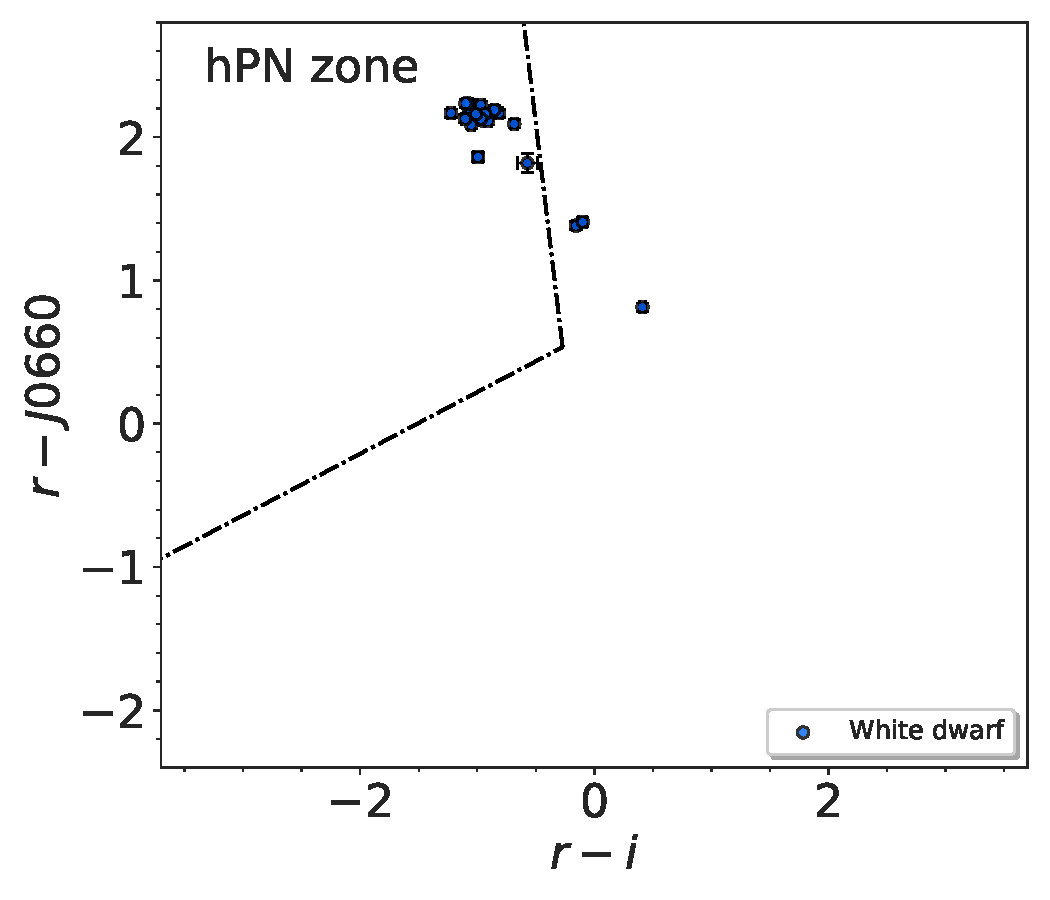
\includegraphics[width=0.5\linewidth, trim=10 10 10 10, clip]{Fig1-IDR2-SPLUS-vironen.pdf} & \\
 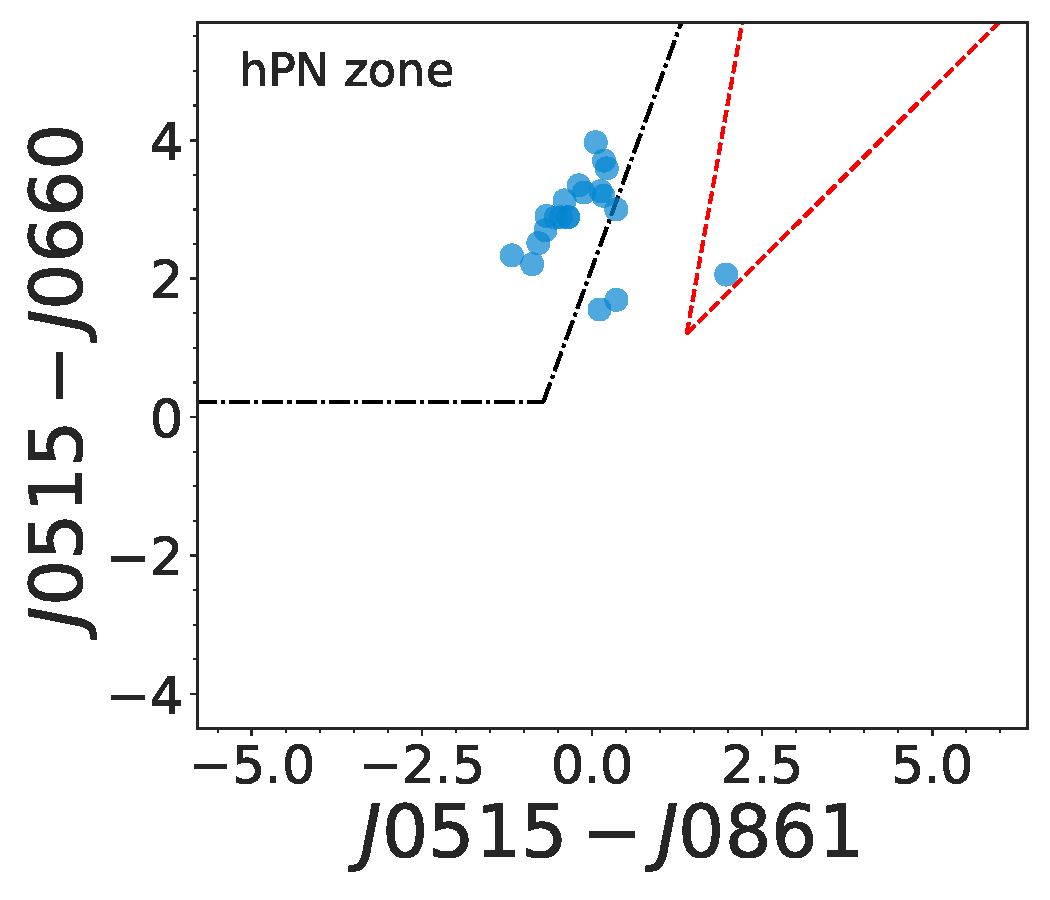
\includegraphics[width=0.5\linewidth, trim=10 10 10 10, clip]{Fig2-IDR2-SPLUS-J0515_J0660.pdf} & 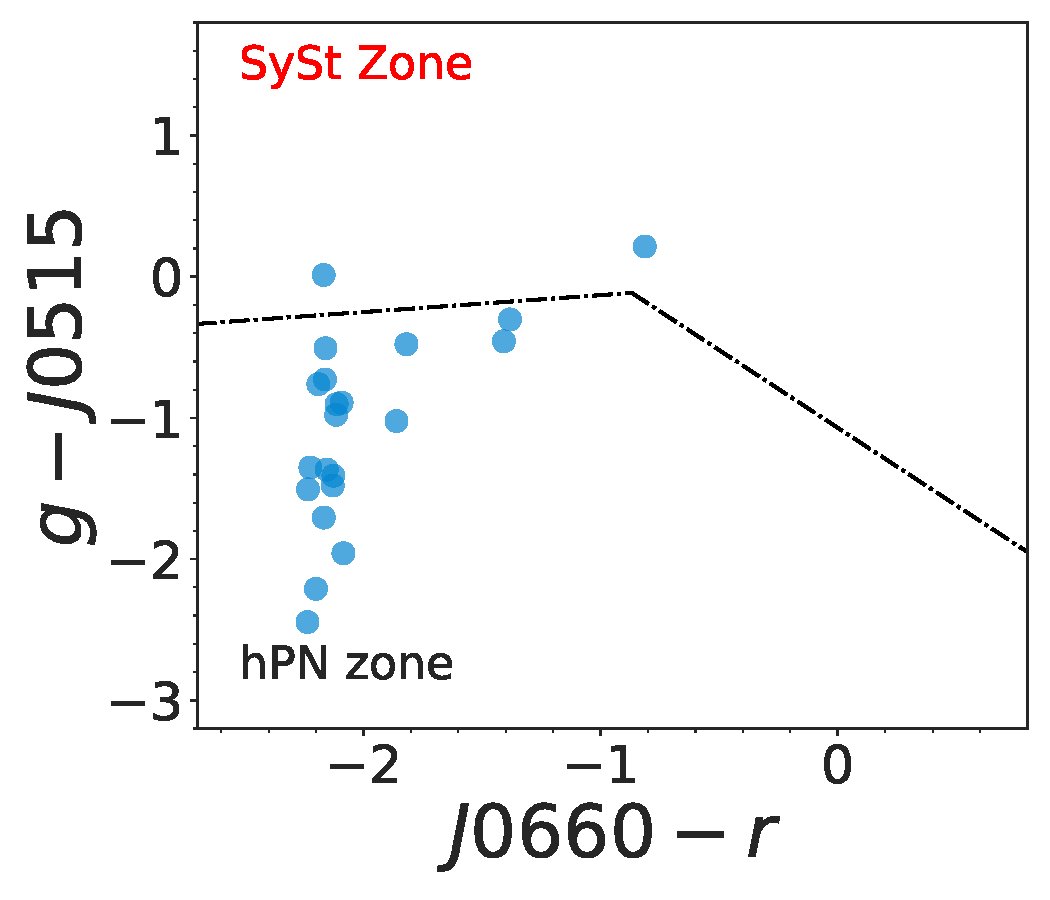
\includegraphics[width=0.5\linewidth, trim=10 10 10 10, clip]{Fig4-IDR2-SPLUS-g.pdf} \\
%\raiselabel{(\textit{a})} & \raiselabel{(\textit{b})}\\
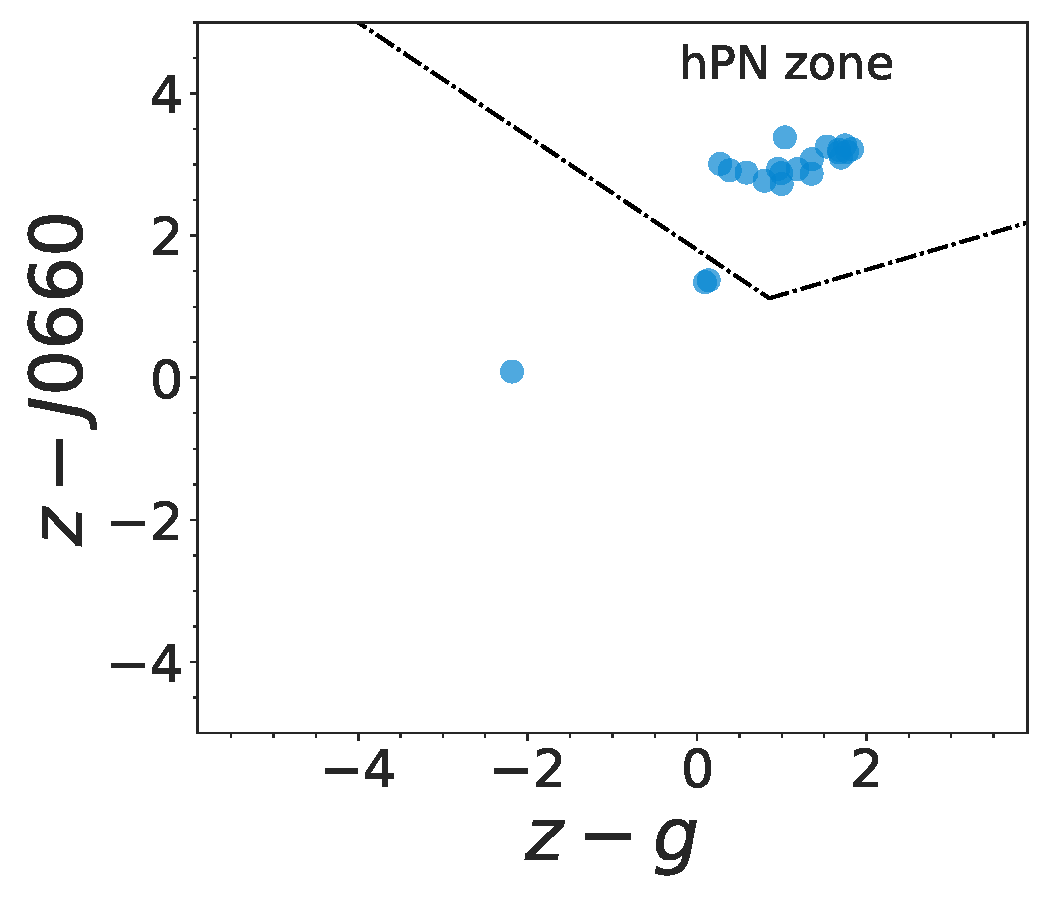
\includegraphics[width=0.5\linewidth, trim=10 10 10 10, clip]{Fig3-IDR2-SPLUS-z.pdf} & 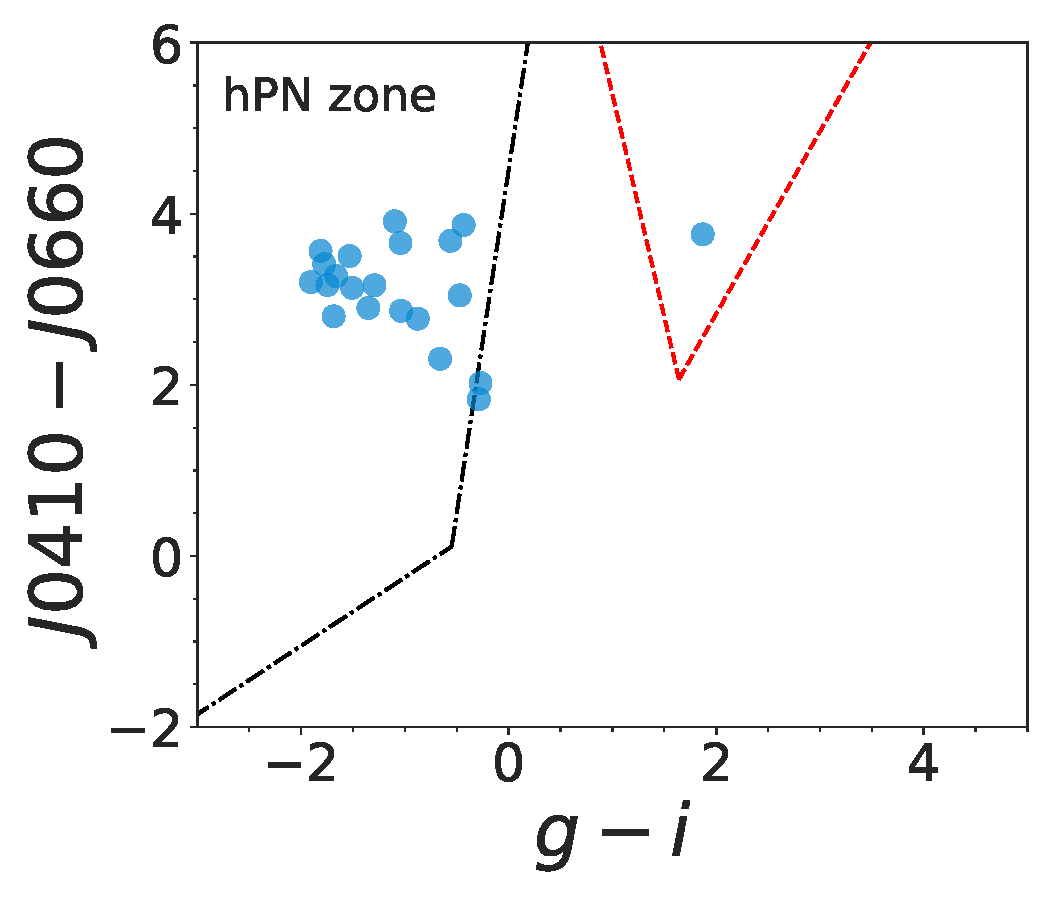
\includegraphics[width=0.5\linewidth, trim=10 10 10 10, clip]{Fig5-IDR2-SPLUS-gi.pdf} \\
%\raiselabel{(\textit{c})} & \raiselabel{(\textit{d})}
\end{tabular}
\caption{}
\label{fig:smppne}
\end{figure*}

The Small Magellanic Cloud (SMC) is a gas-rich late-type dwarf galaxy (Bolatto et al. 2007) with a gas-to-dust ratio 30 times higher than the Milky Way (Stanimirovic et al. 2000). It is a member of the Local Group and is classified as an irregular galaxy (ImIV$-$V) (Sandage et al. 1994). The SMC is at a distance of 60.6$\pm$3.8 kpc (Hilditch et al. 2005) from the Galaxy which makes the spatial scale $\sim$0.3 pc$/$arcsec.

I found this sample of SMC PNe: vizier -$>$ \url{J/A+A/472/101/table7}. Chemical evolution of SMC planetary nebulae (Idiart+, 2007, \url{2007A&A...472..101I}) This catalog has $\sim$40 PNe.\\

I made cross matching between this catalog and SPLUS catalog. I found 21 matches using a 1 arcsec of radii. 

I putted the final matches in my S-PLUS colour diagrams diagram (see Fig.~\ref{fig:smppne}),


\newpage
\begin{longtable}{ccc}
  %\caption[]{continuación }\\
  \begin{table}
\begin{tabular}{ccc}
\textbf{Aper} & \textbf{Auto} & \textbf{Petro} \\
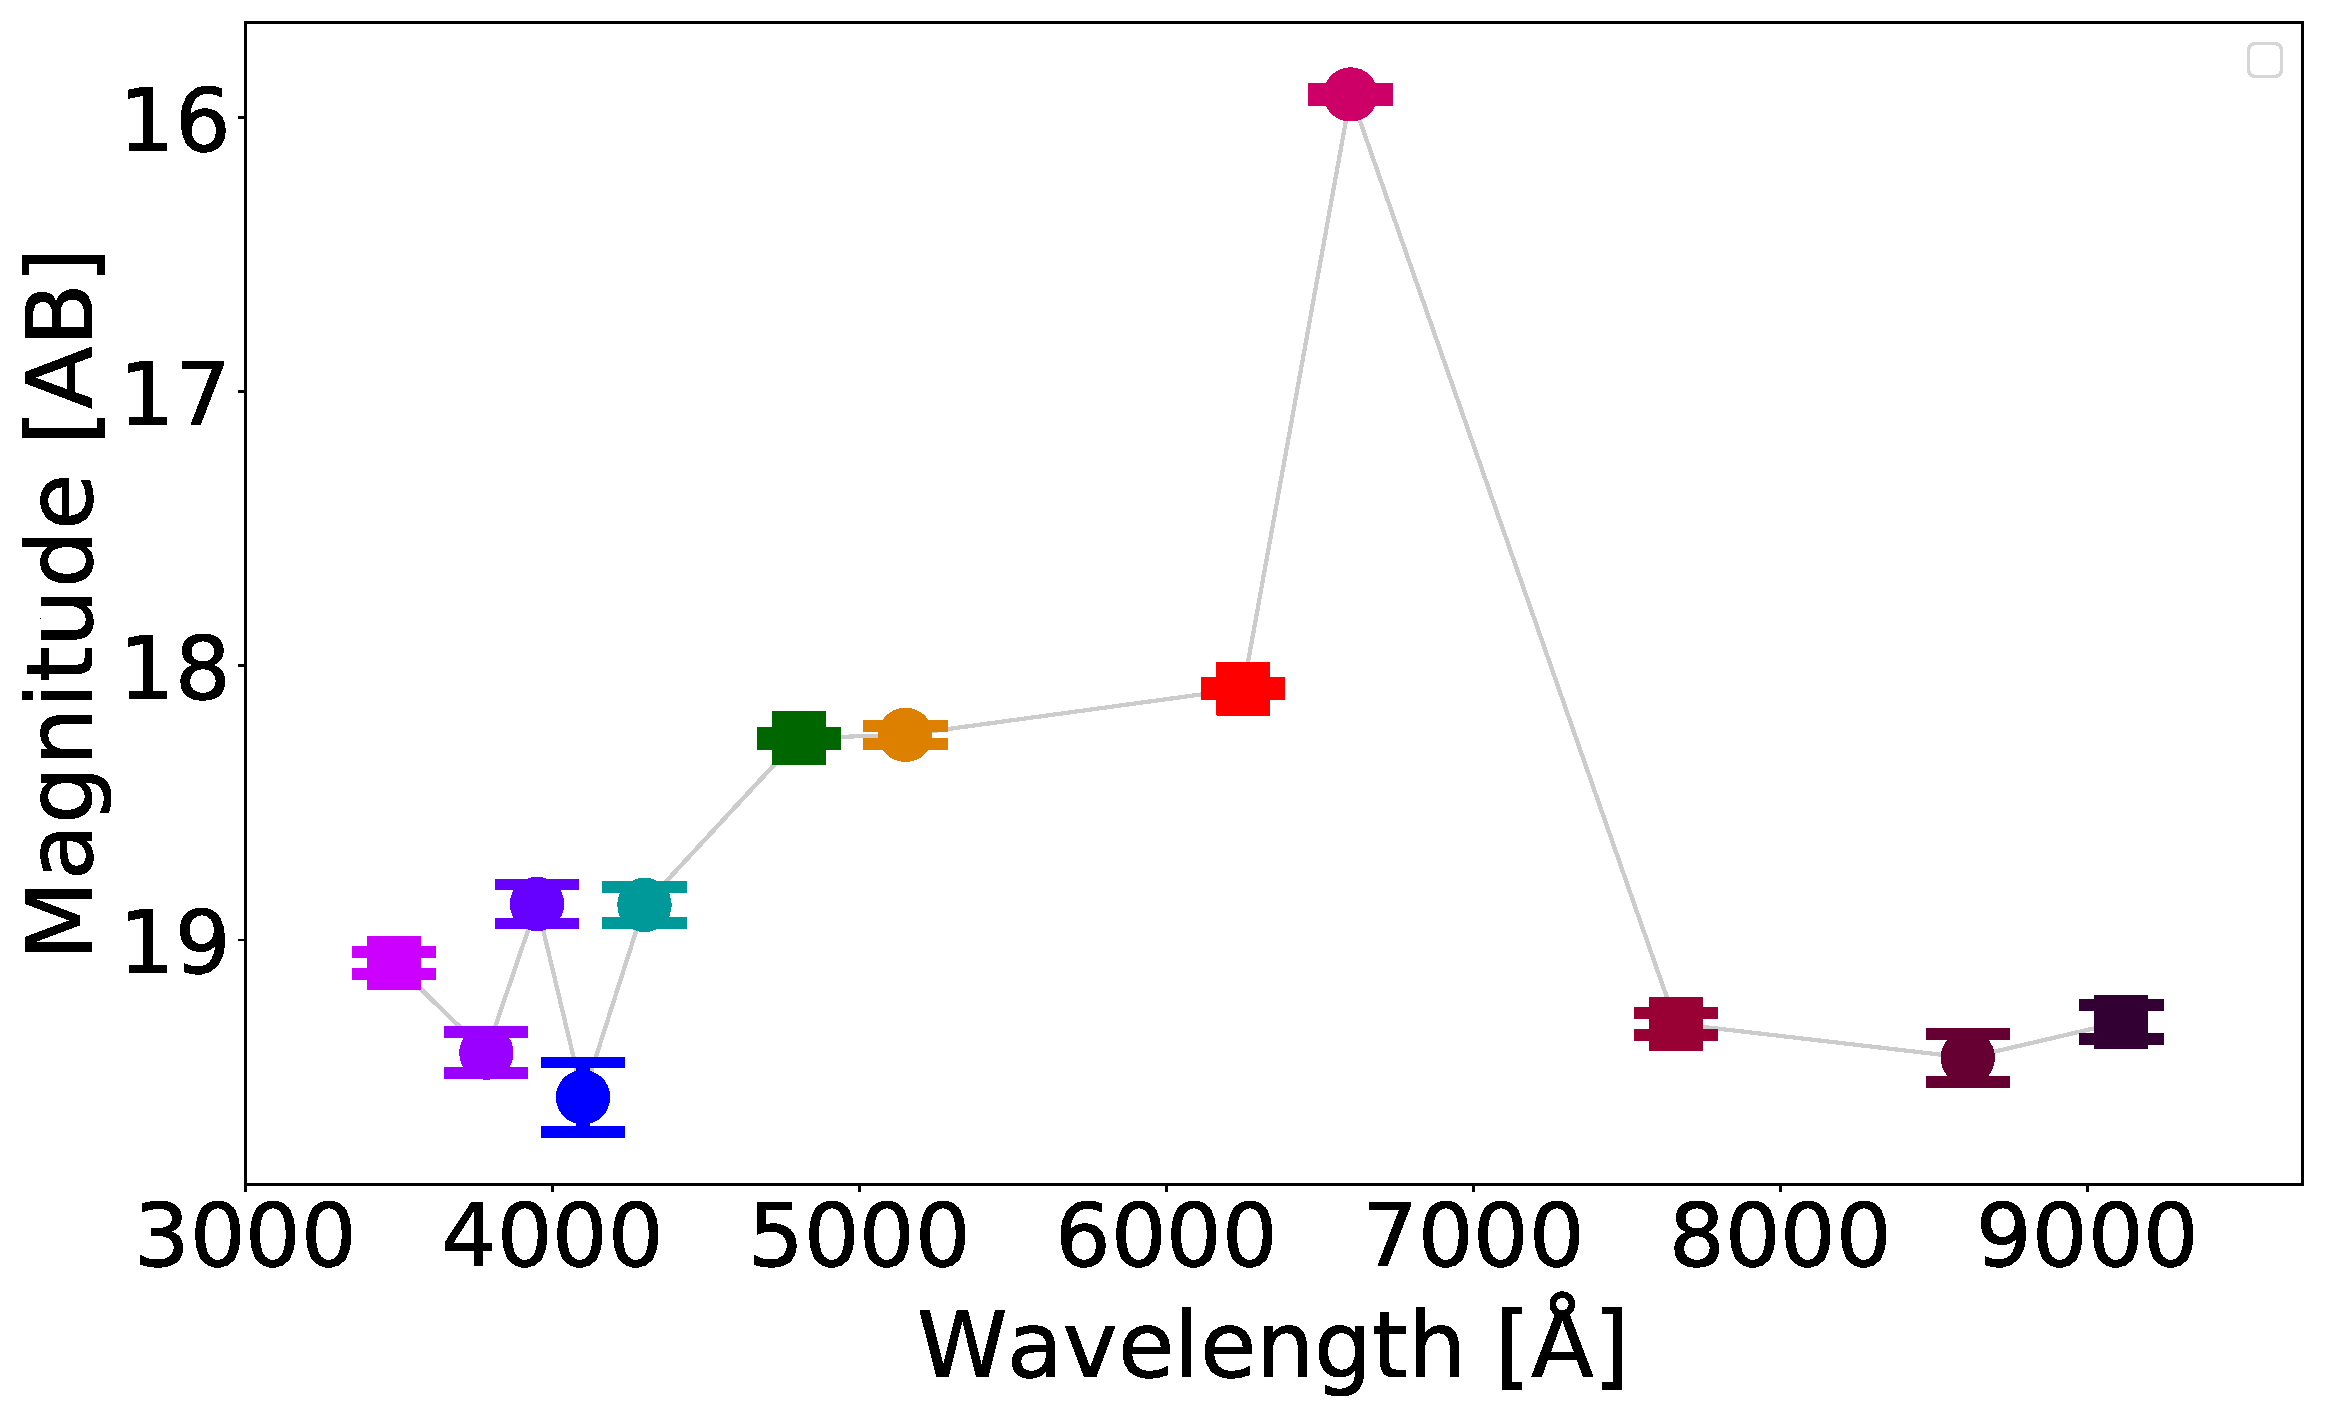
\includegraphics[width=0.3\linewidth, clip]{photopectrum_splus_MC0072-006125_aper.pdf} & 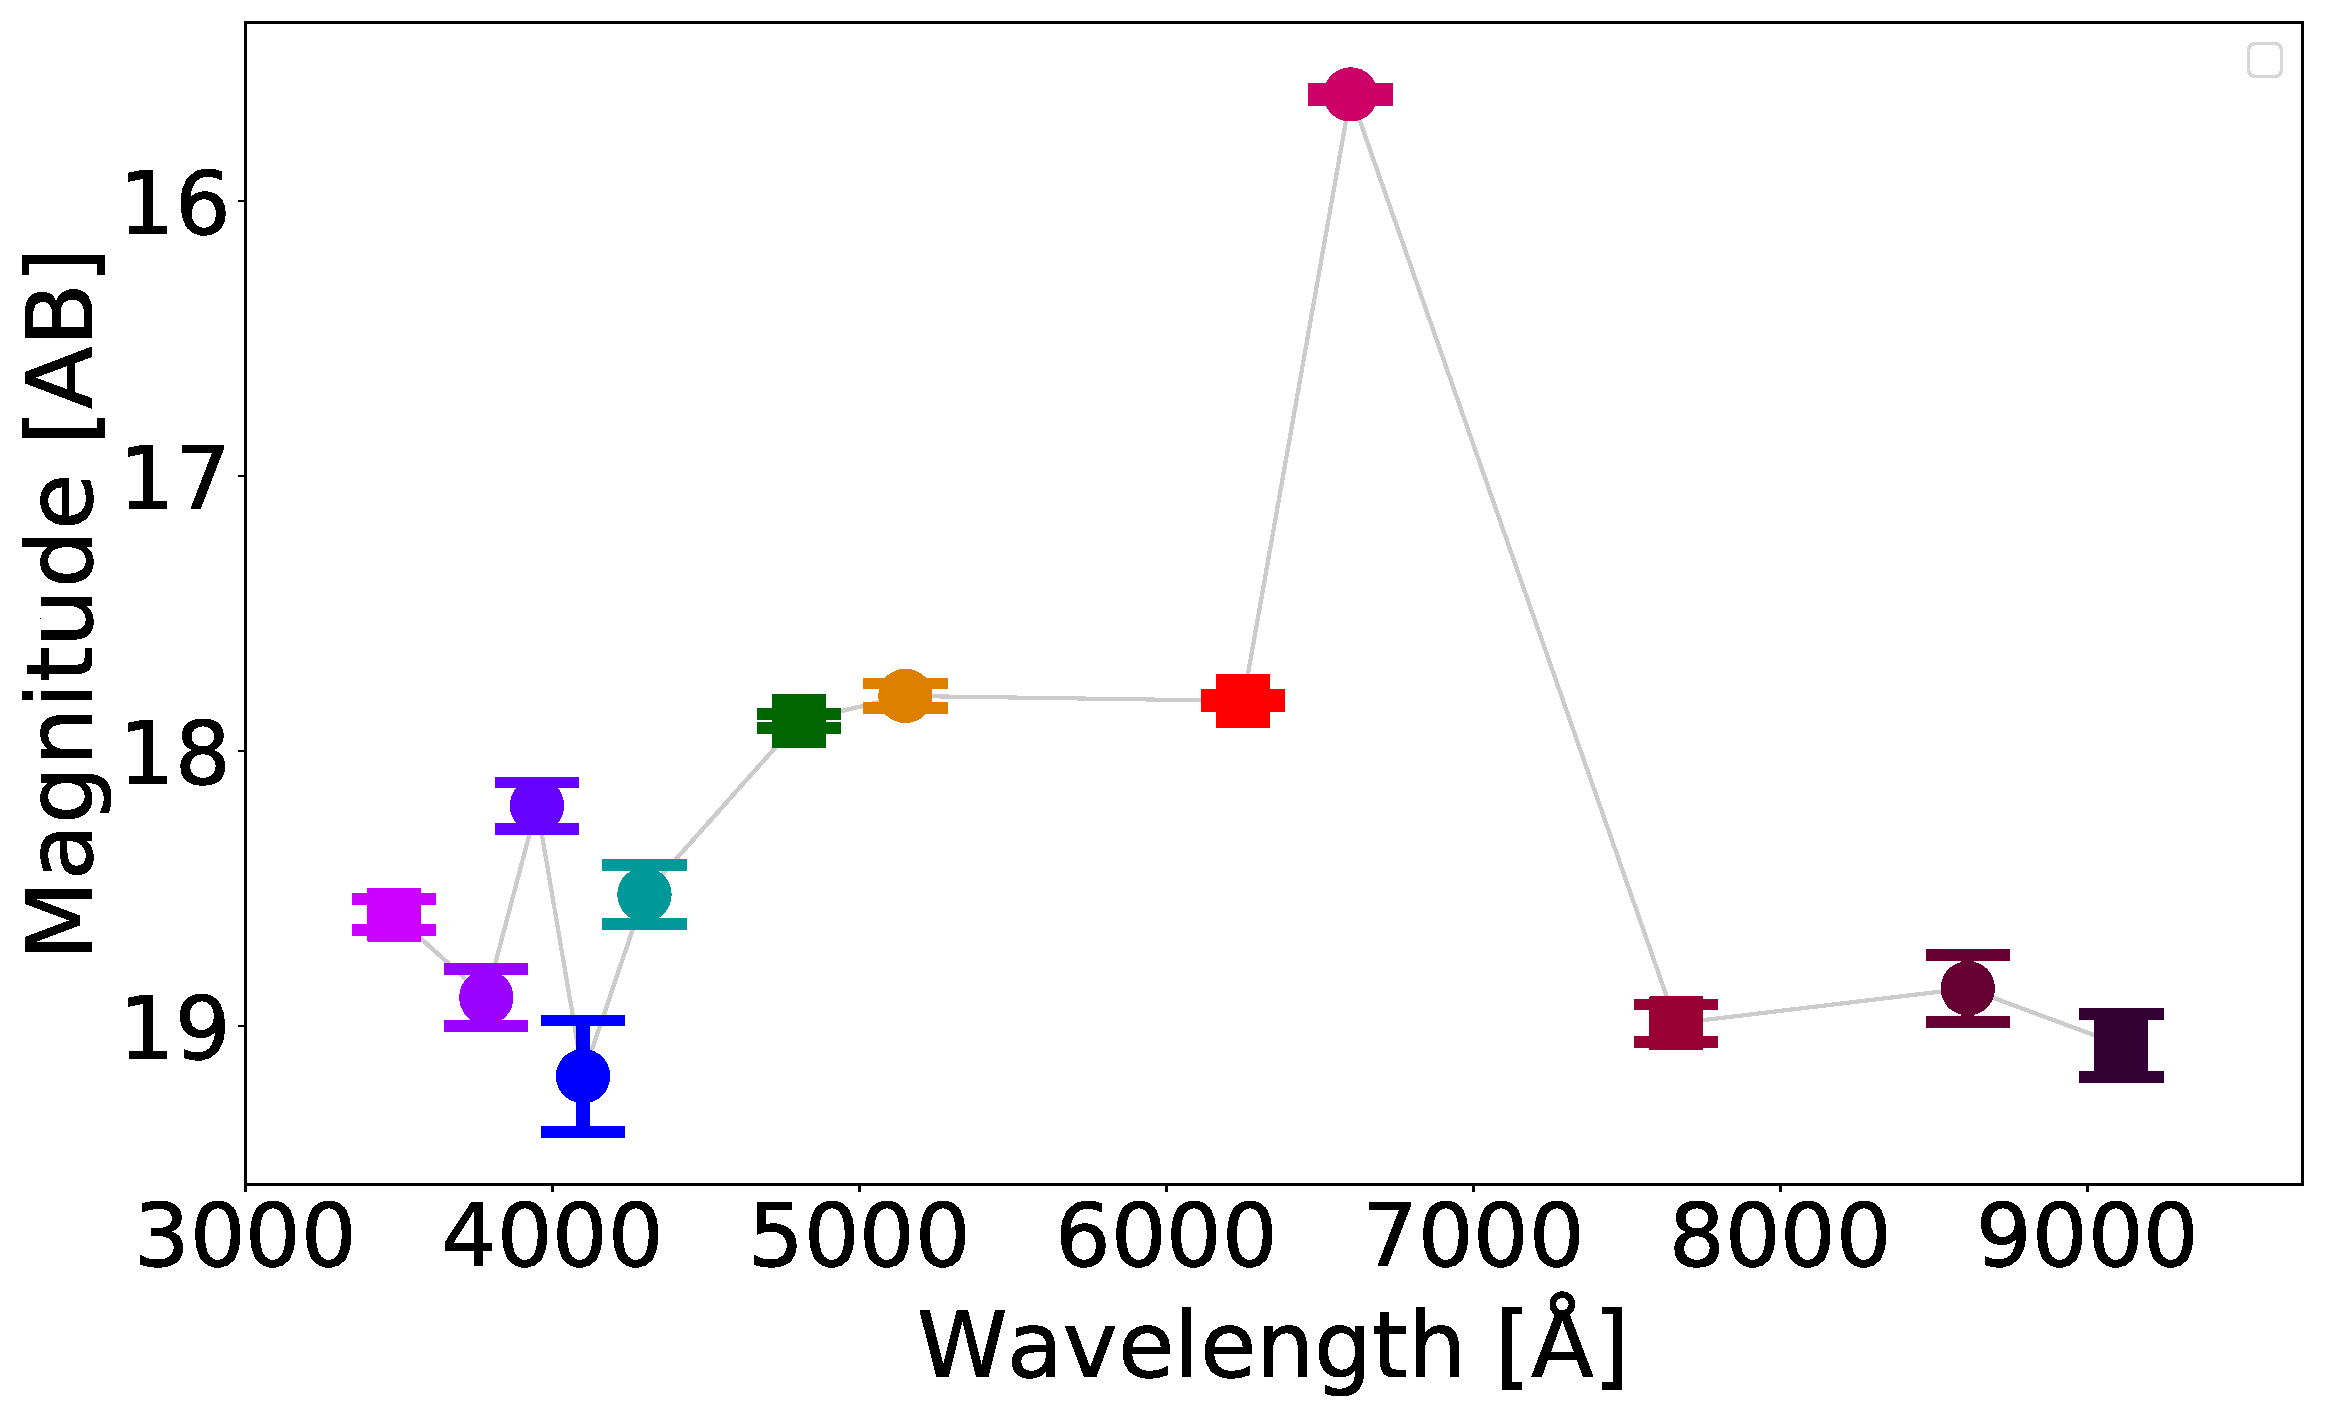
\includegraphics[width=0.3\linewidth, clip]{photopectrum_splus_MC0072-006125_auto.pdf} & 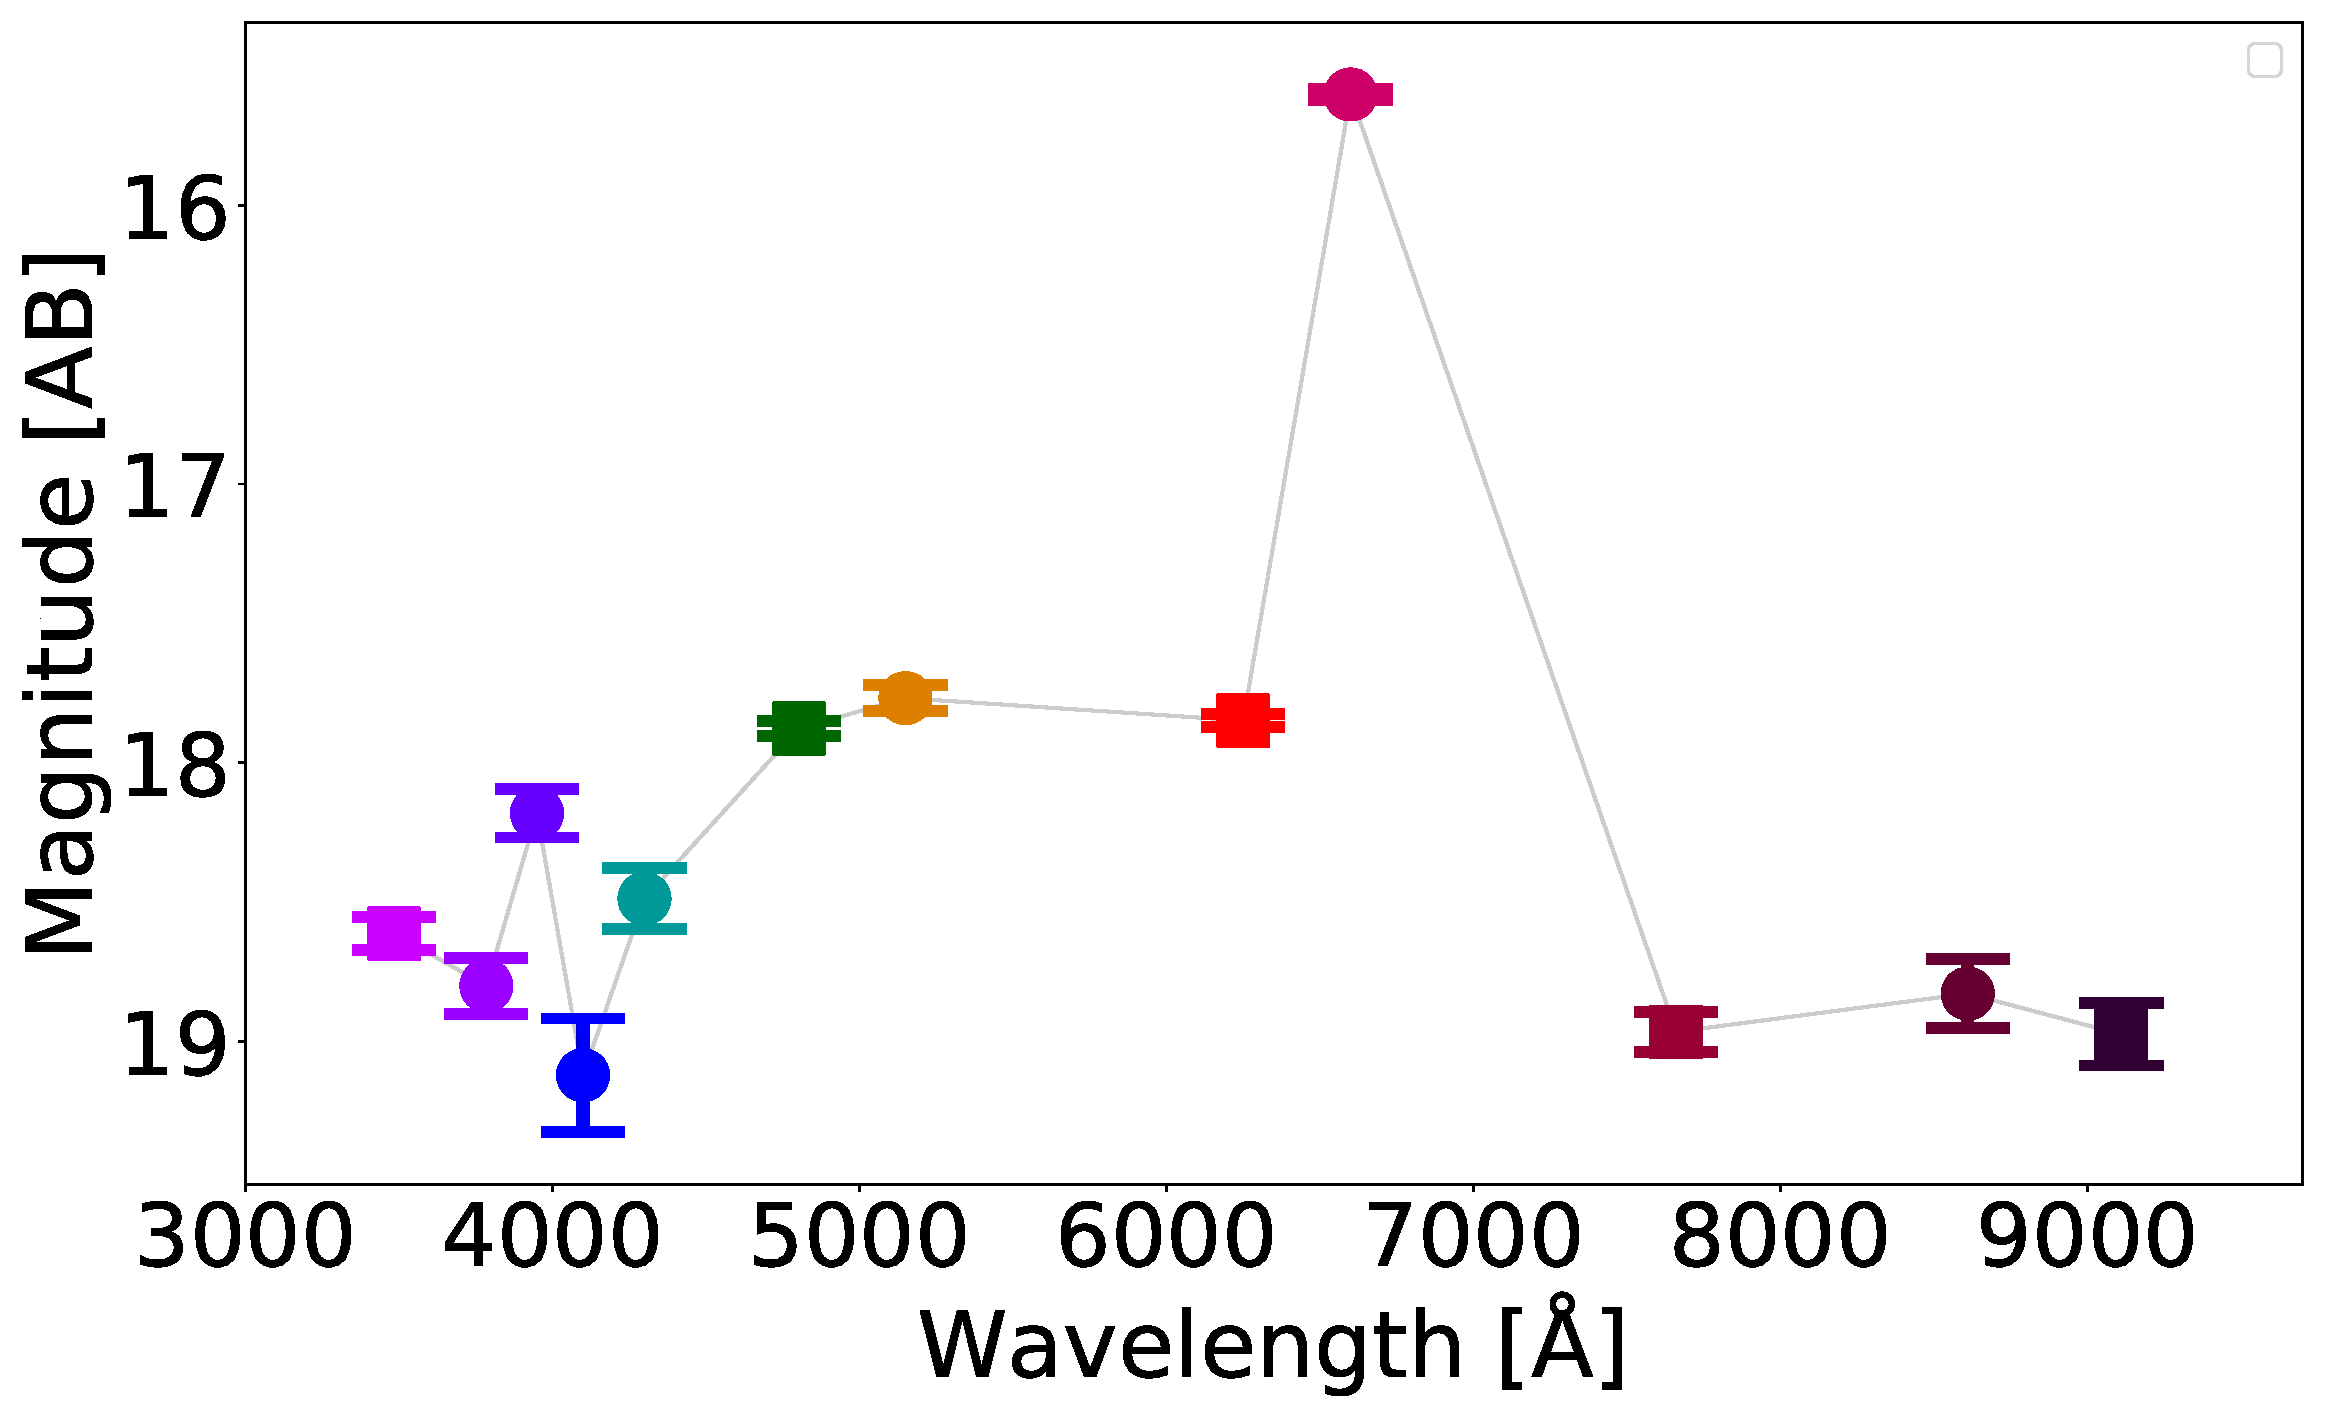
\includegraphics[width=0.3\linewidth, clip]{photopectrum_splus_MC0072-006125_petro.pdf} \\
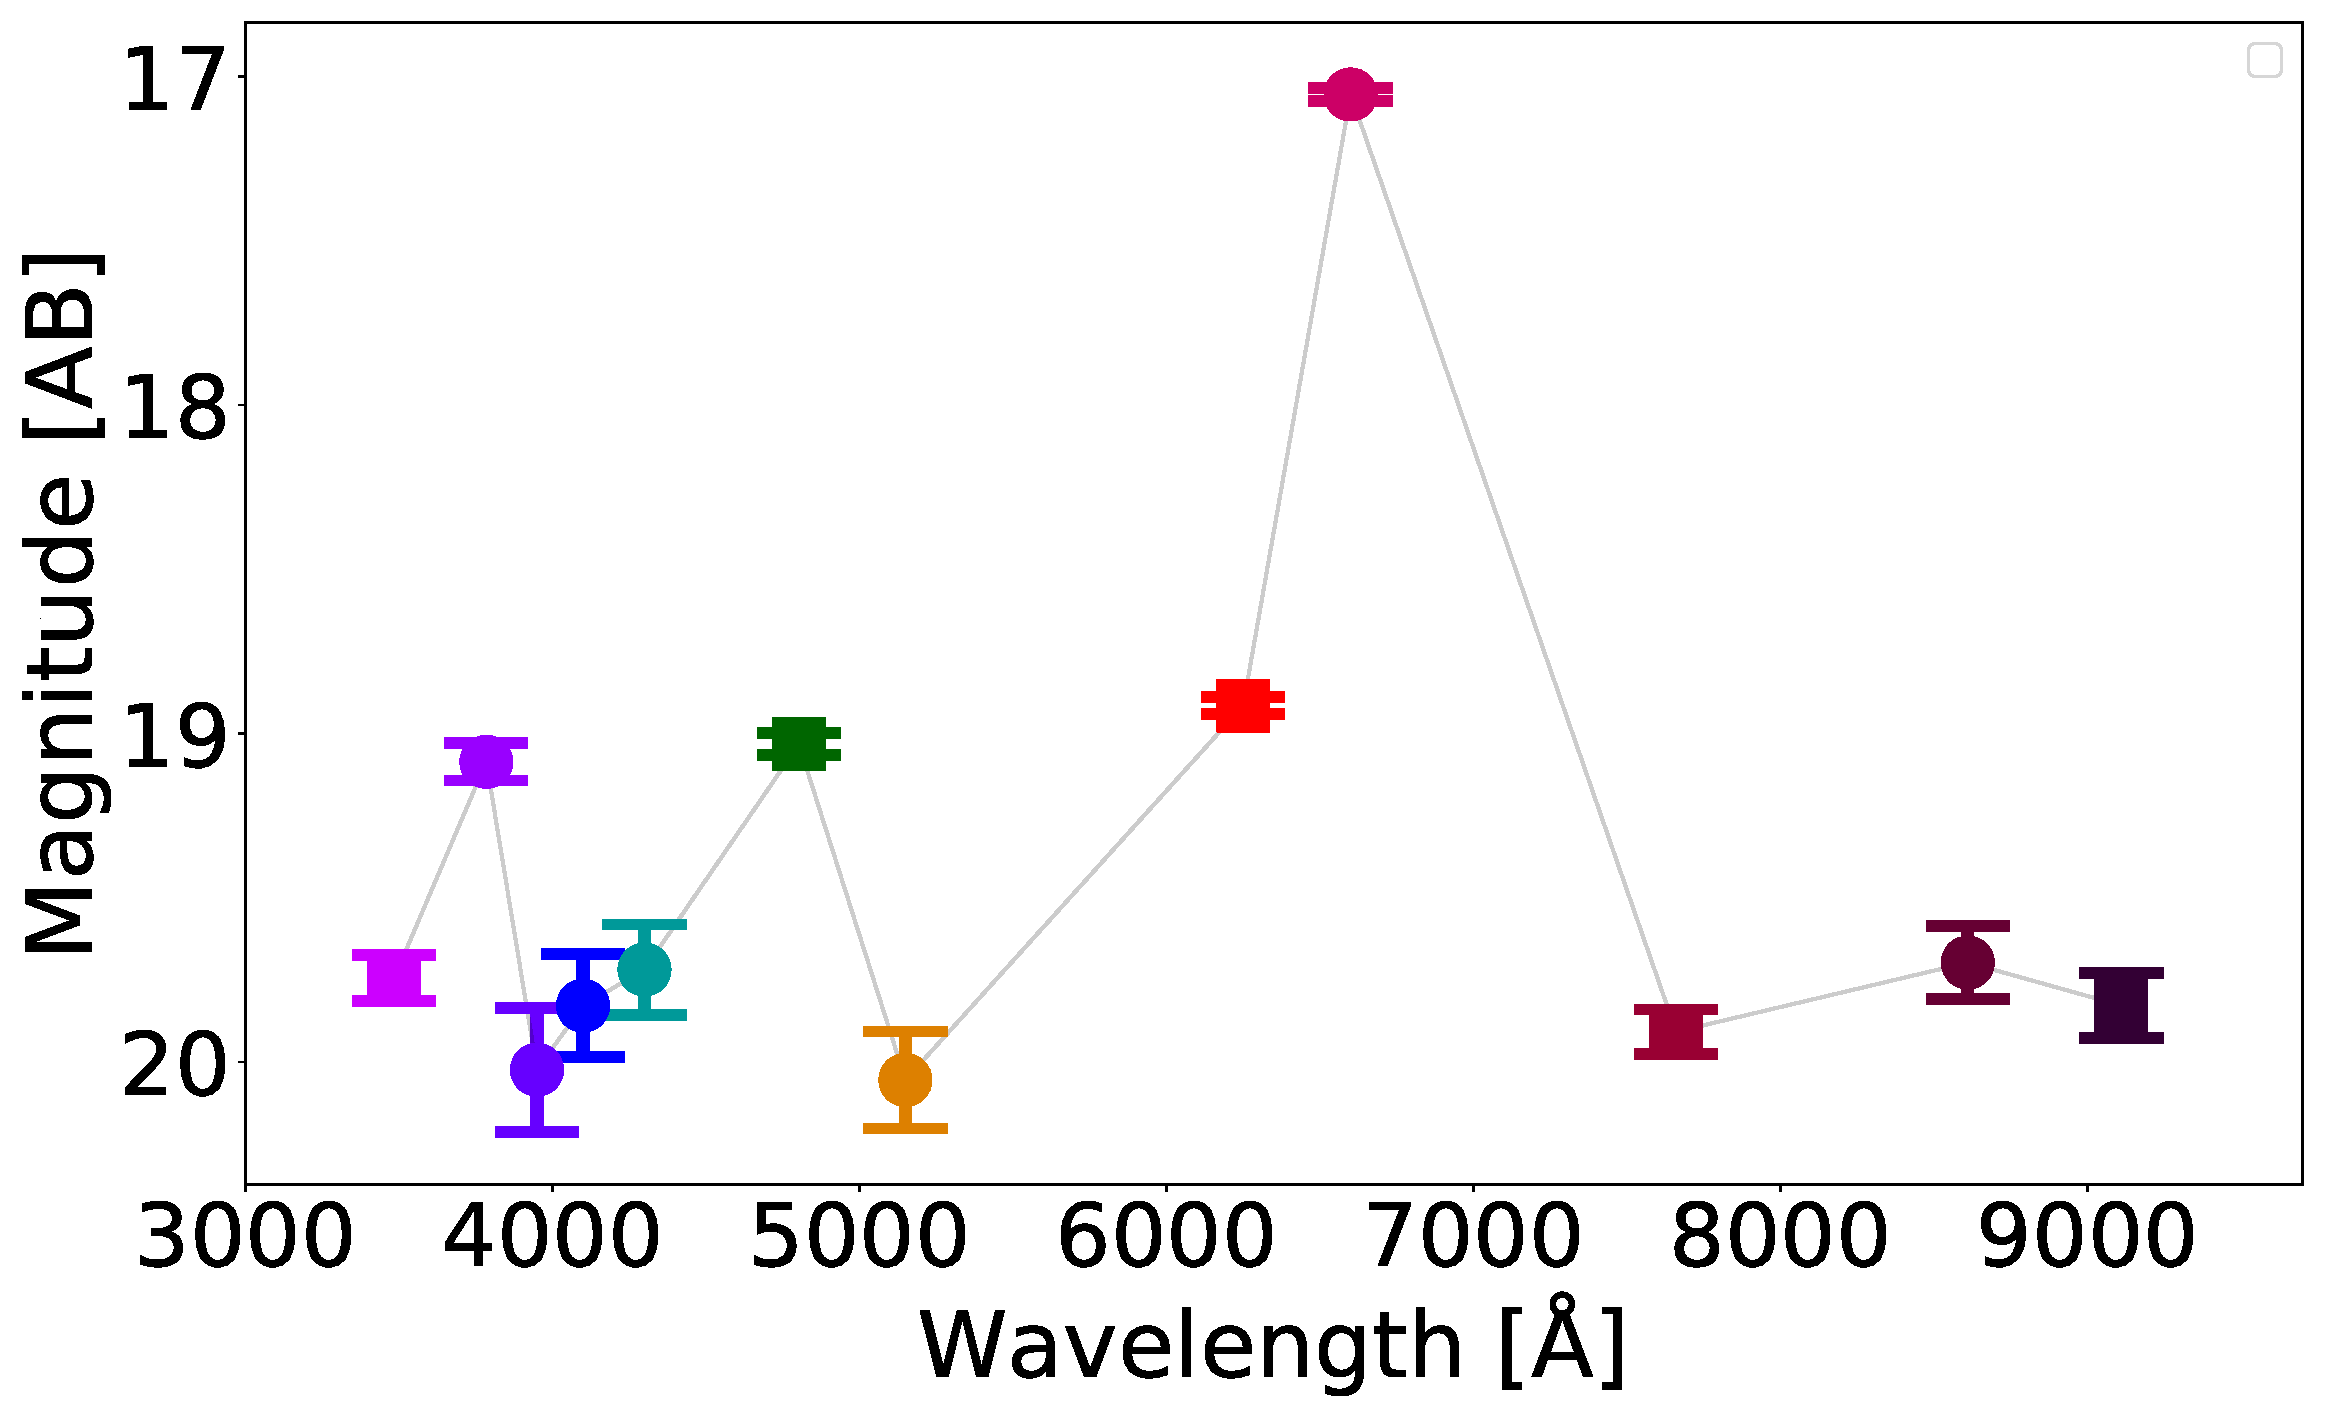
\includegraphics[width=0.3\linewidth, clip]{photopectrum_splus_MC0072-044863_aper.pdf} & 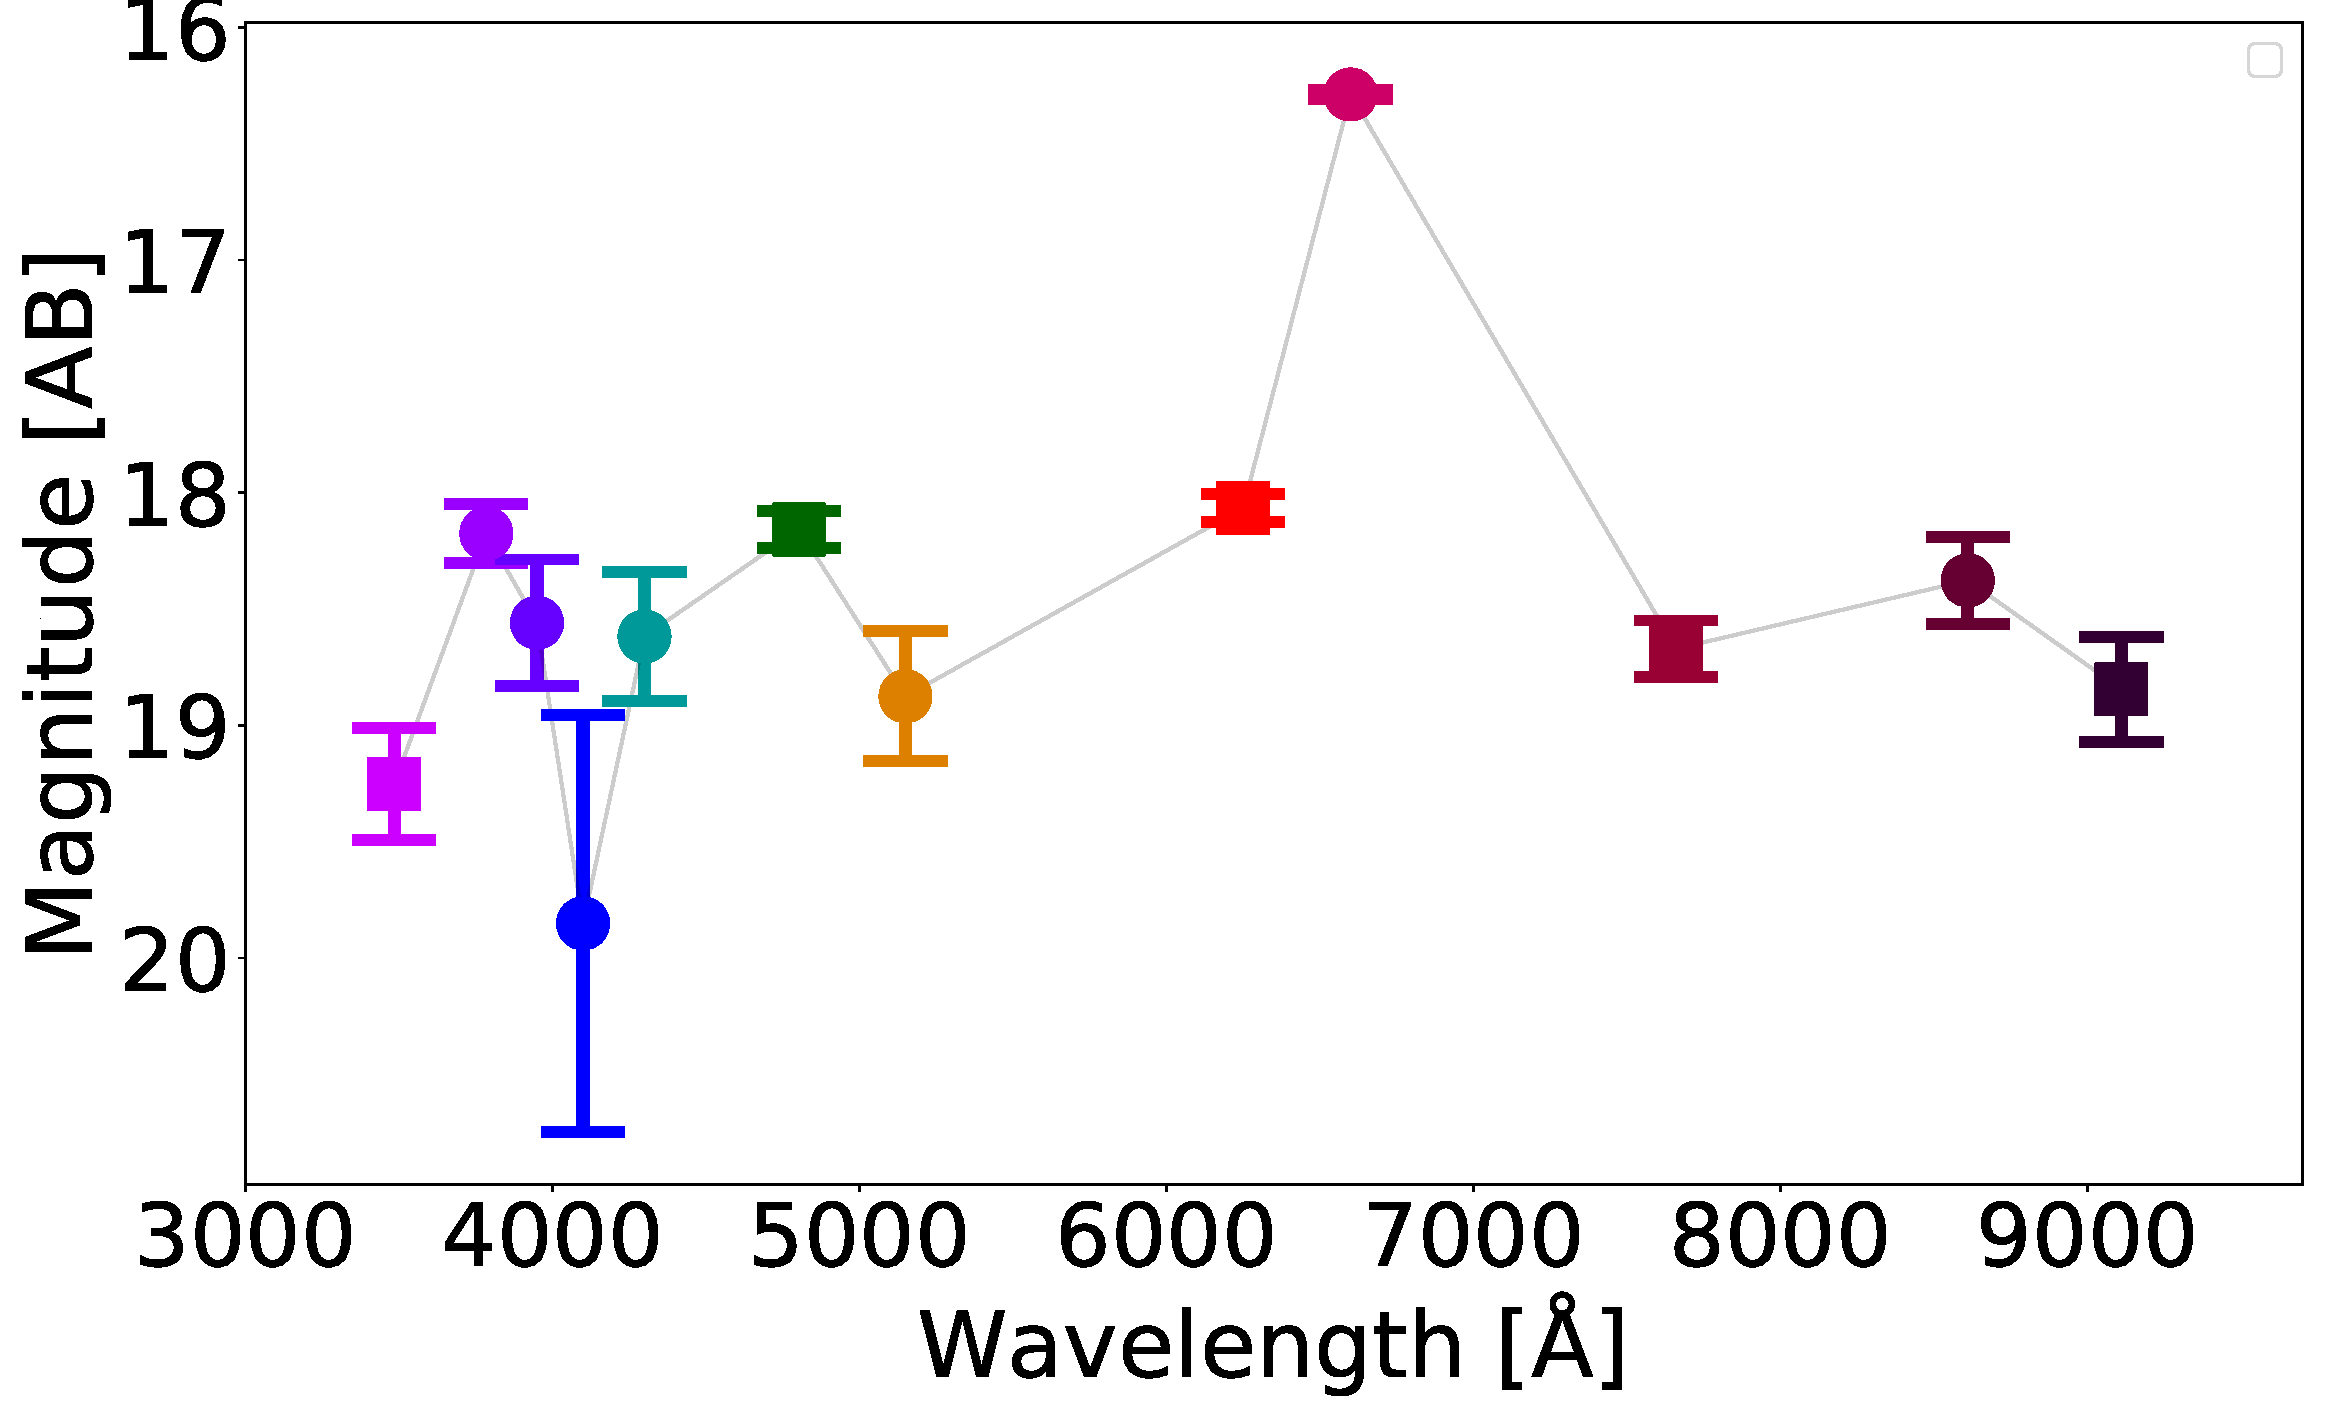
\includegraphics[width=0.3\linewidth, clip]{photopectrum_splus_MC0072-044863_auto.pdf} & 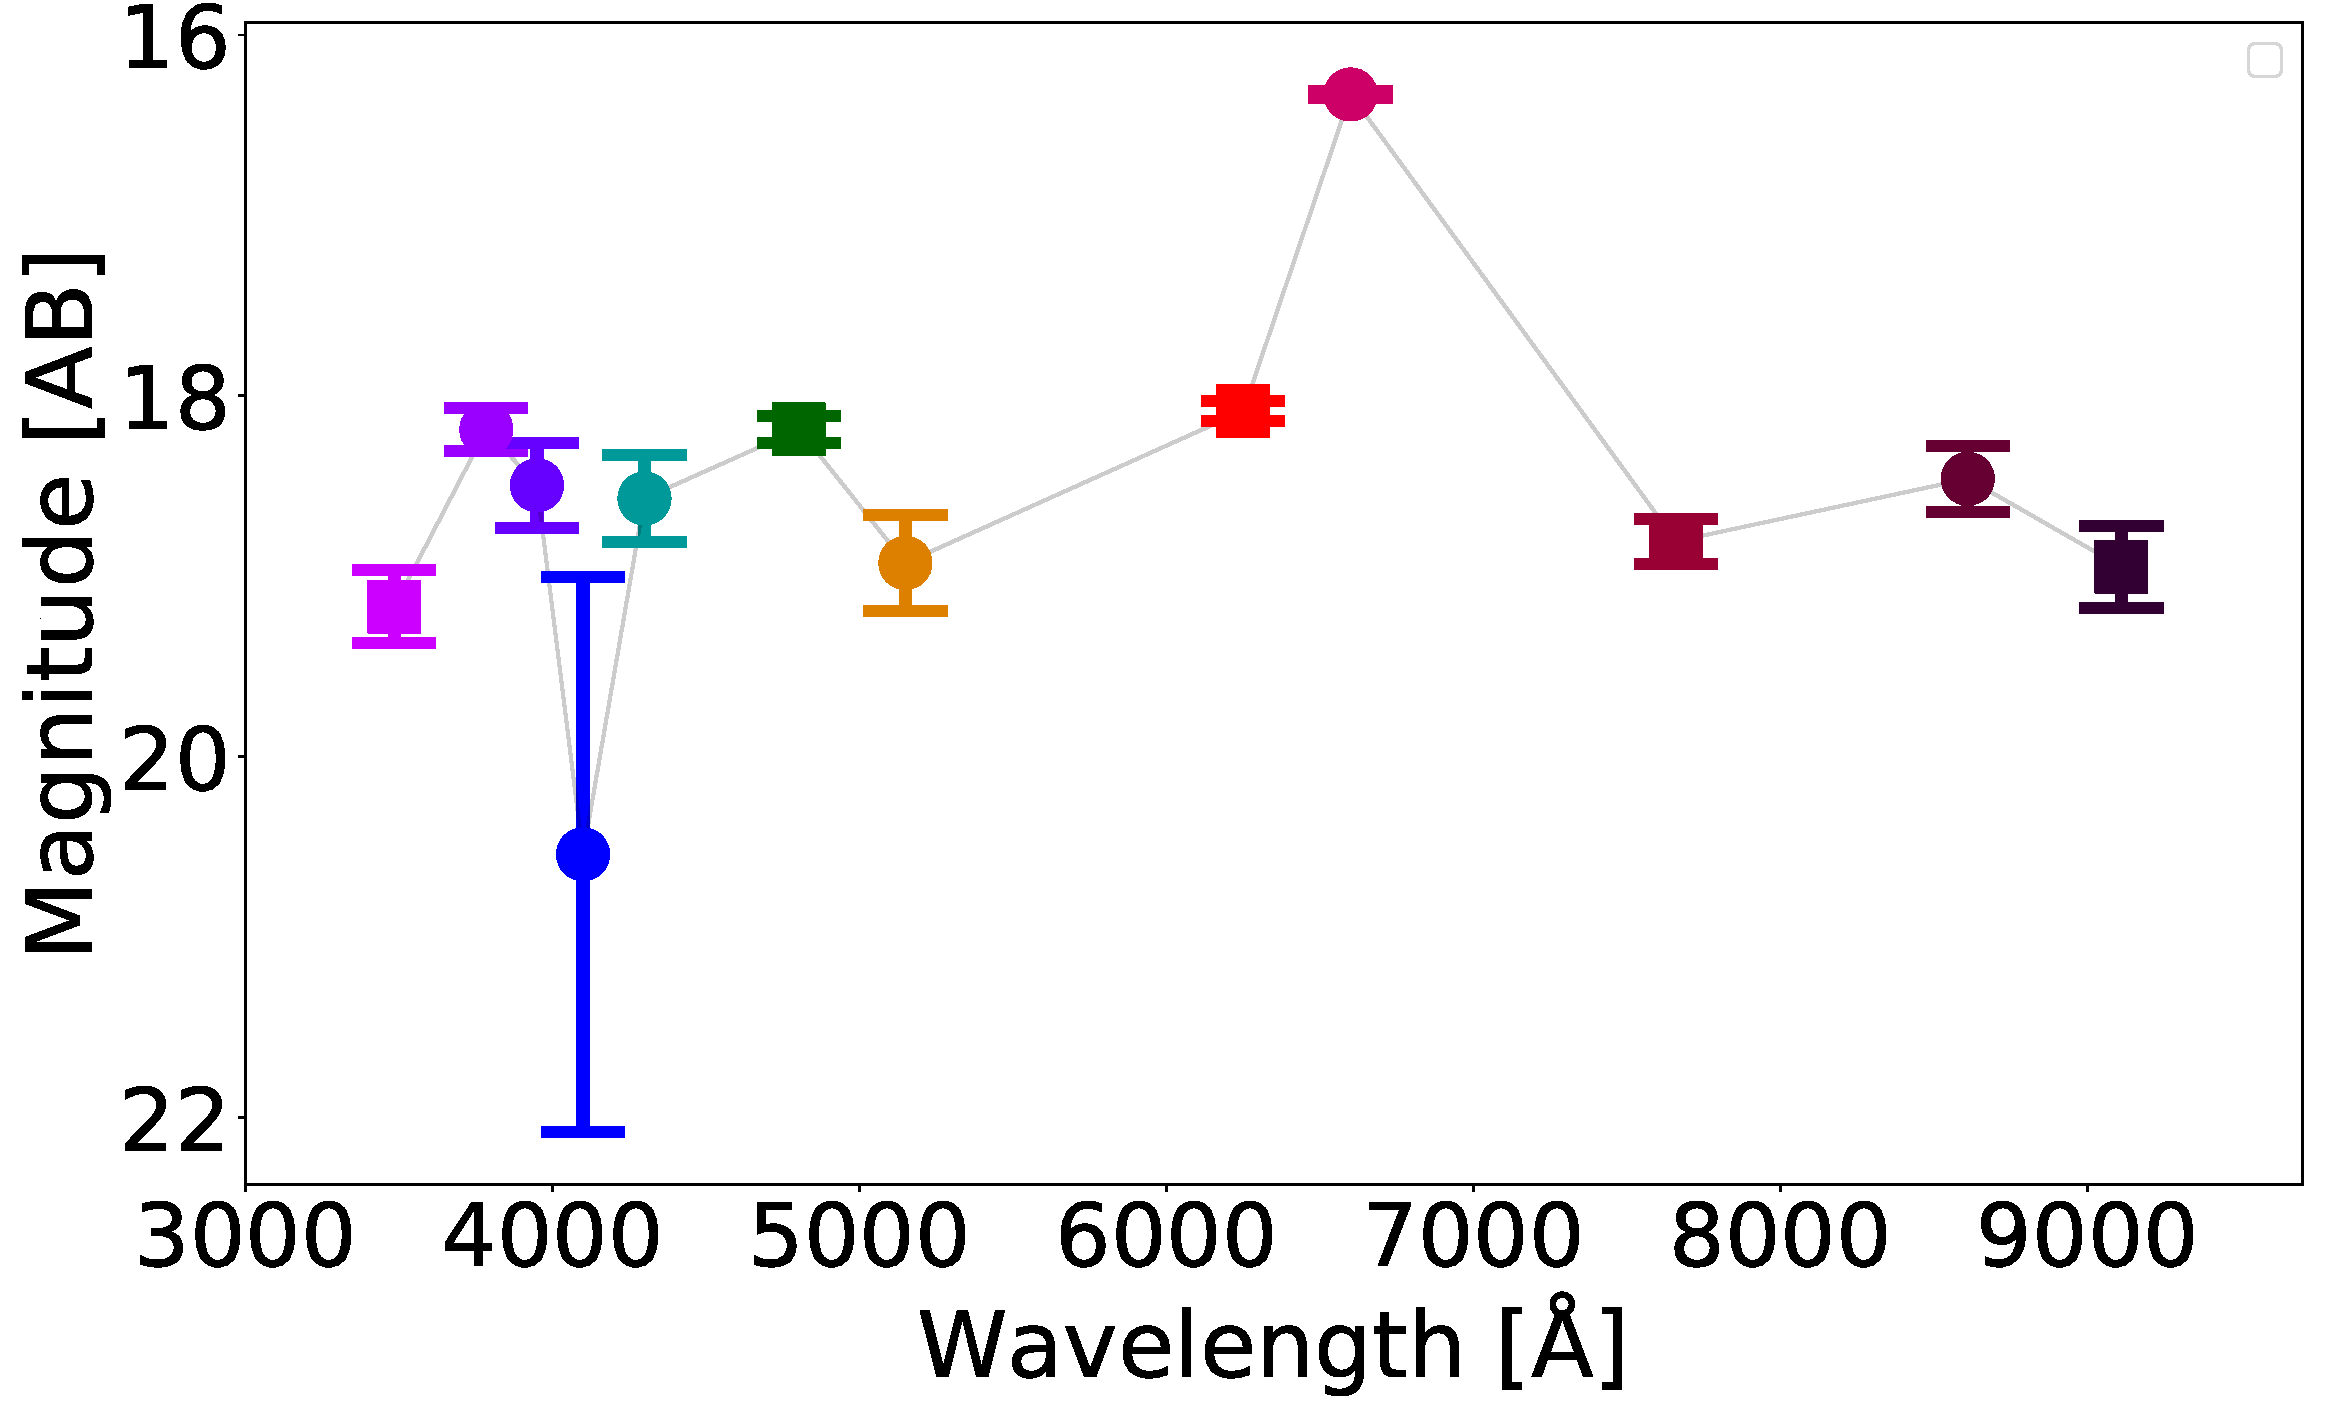
\includegraphics[width=0.3\linewidth, clip]{photopectrum_splus_MC0072-044863_petro.pdf} \\
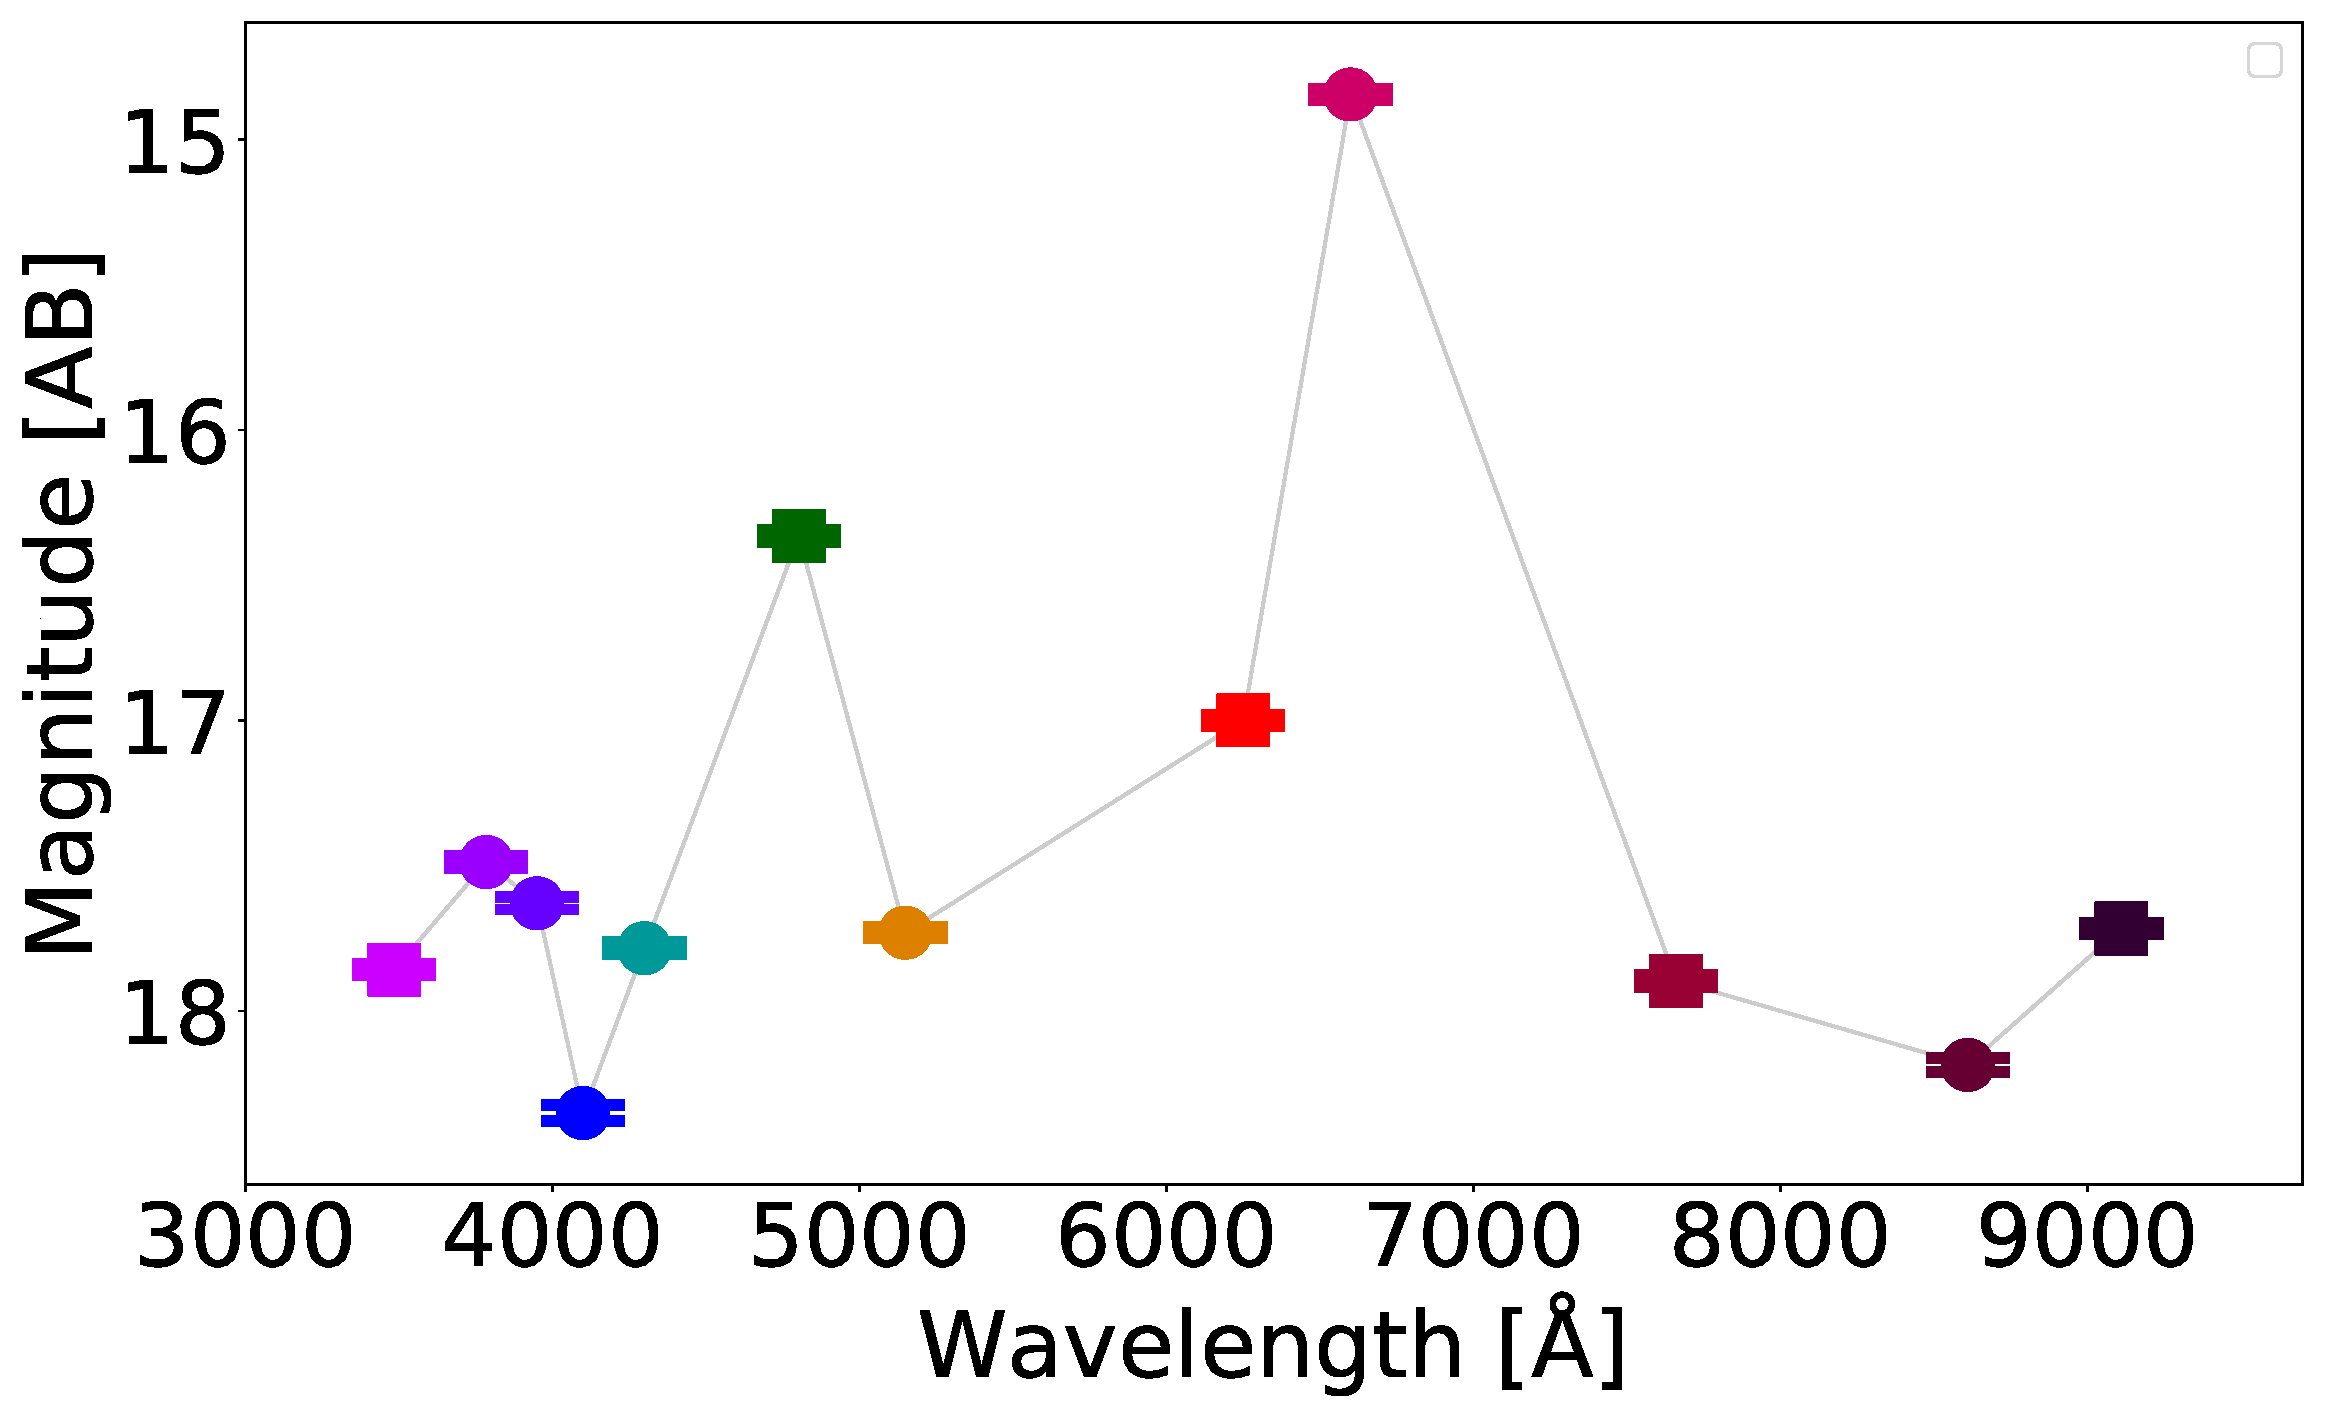
\includegraphics[width=0.3\linewidth, clip]{photopectrum_splus_MC0093-051819_aper.pdf} & 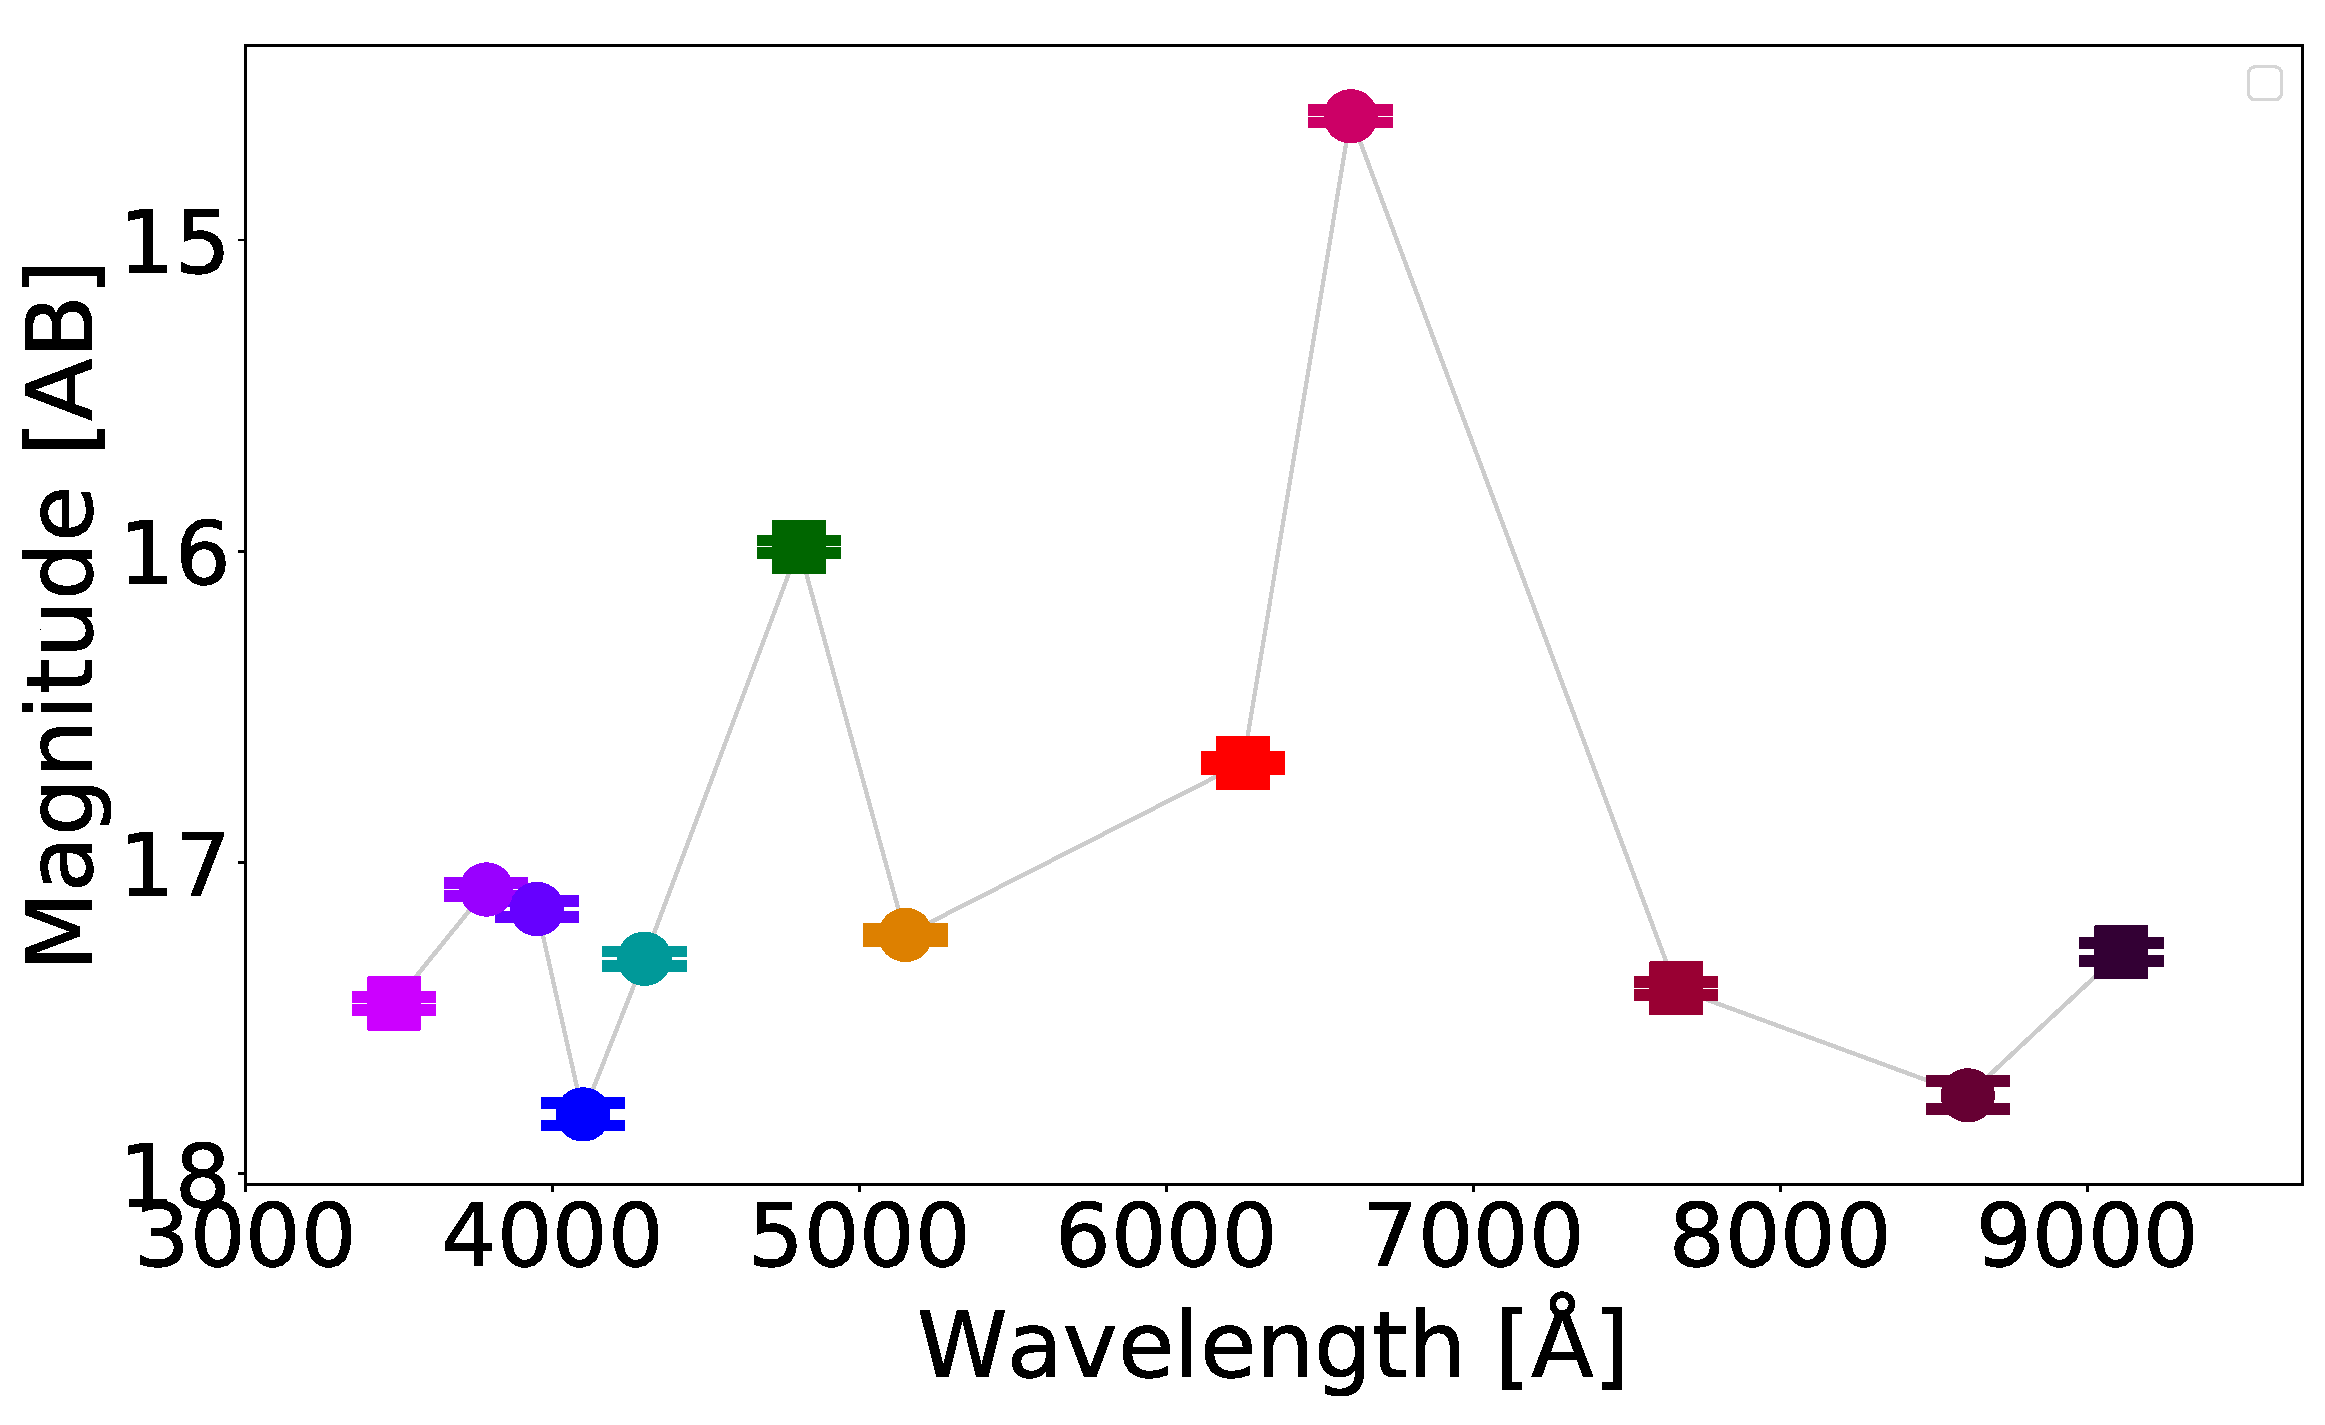
\includegraphics[width=0.3\linewidth, clip]{photopectrum_splus_MC0093-051819_auto.pdf} & 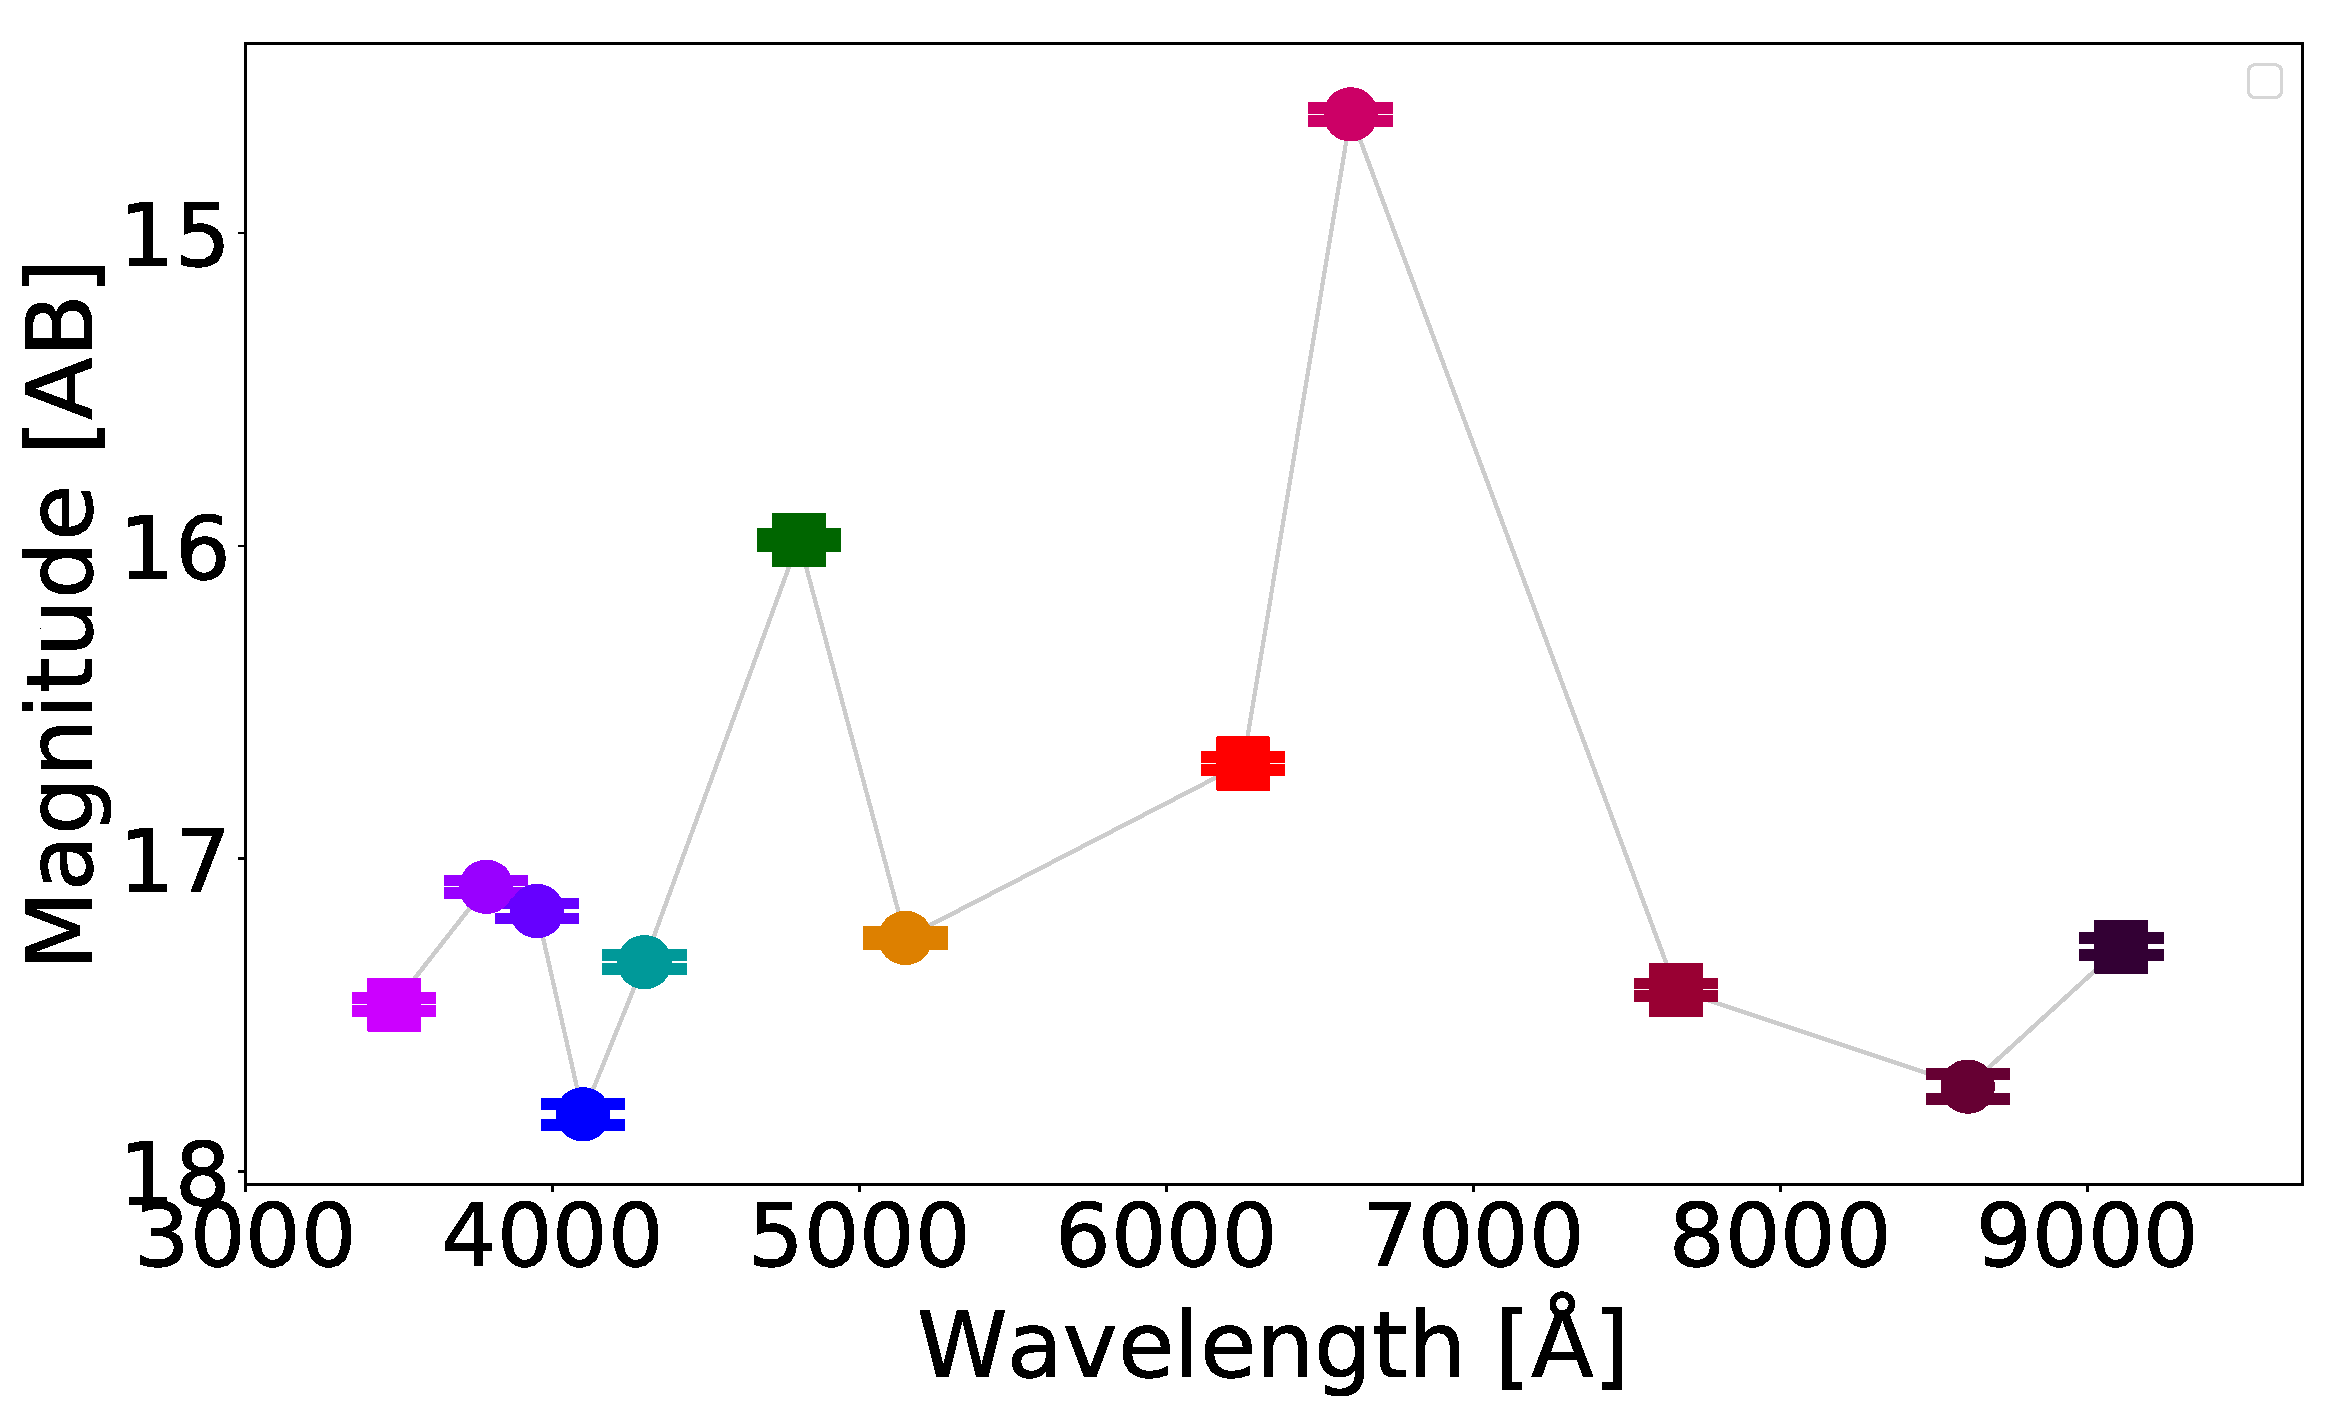
\includegraphics[width=0.3\linewidth, clip]{photopectrum_splus_MC0093-051819_petro.pdf} \\
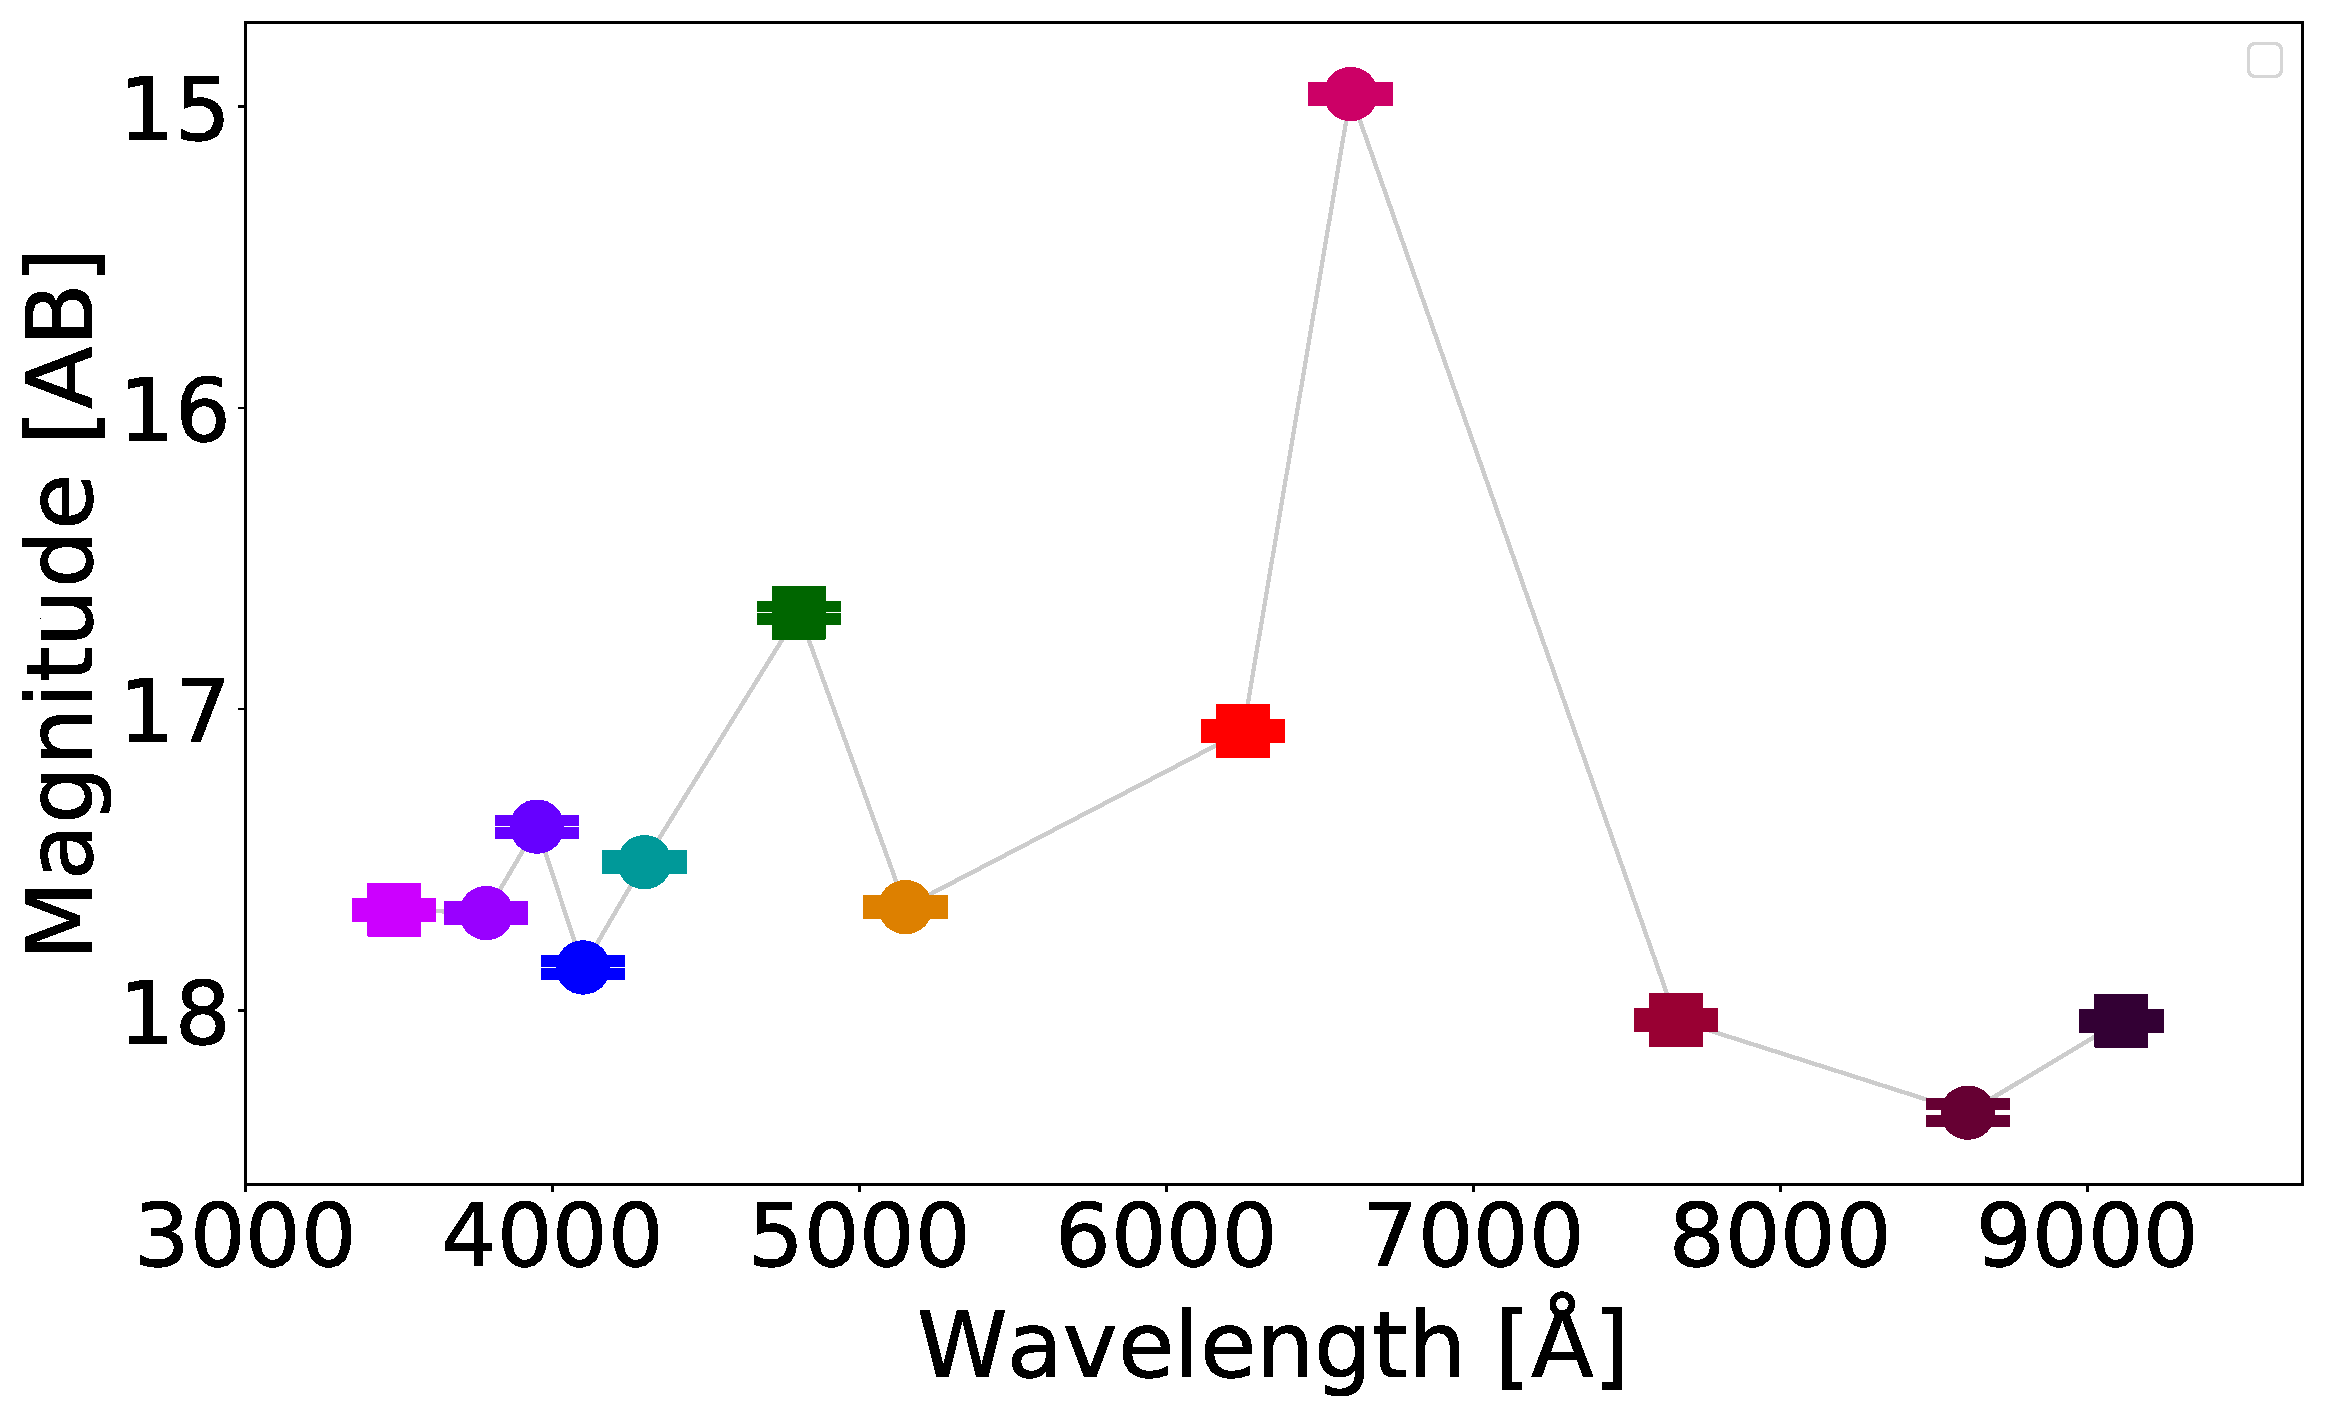
\includegraphics[width=0.3\linewidth, clip]{photopectrum_splus_MC0093-085620_aper.pdf} & 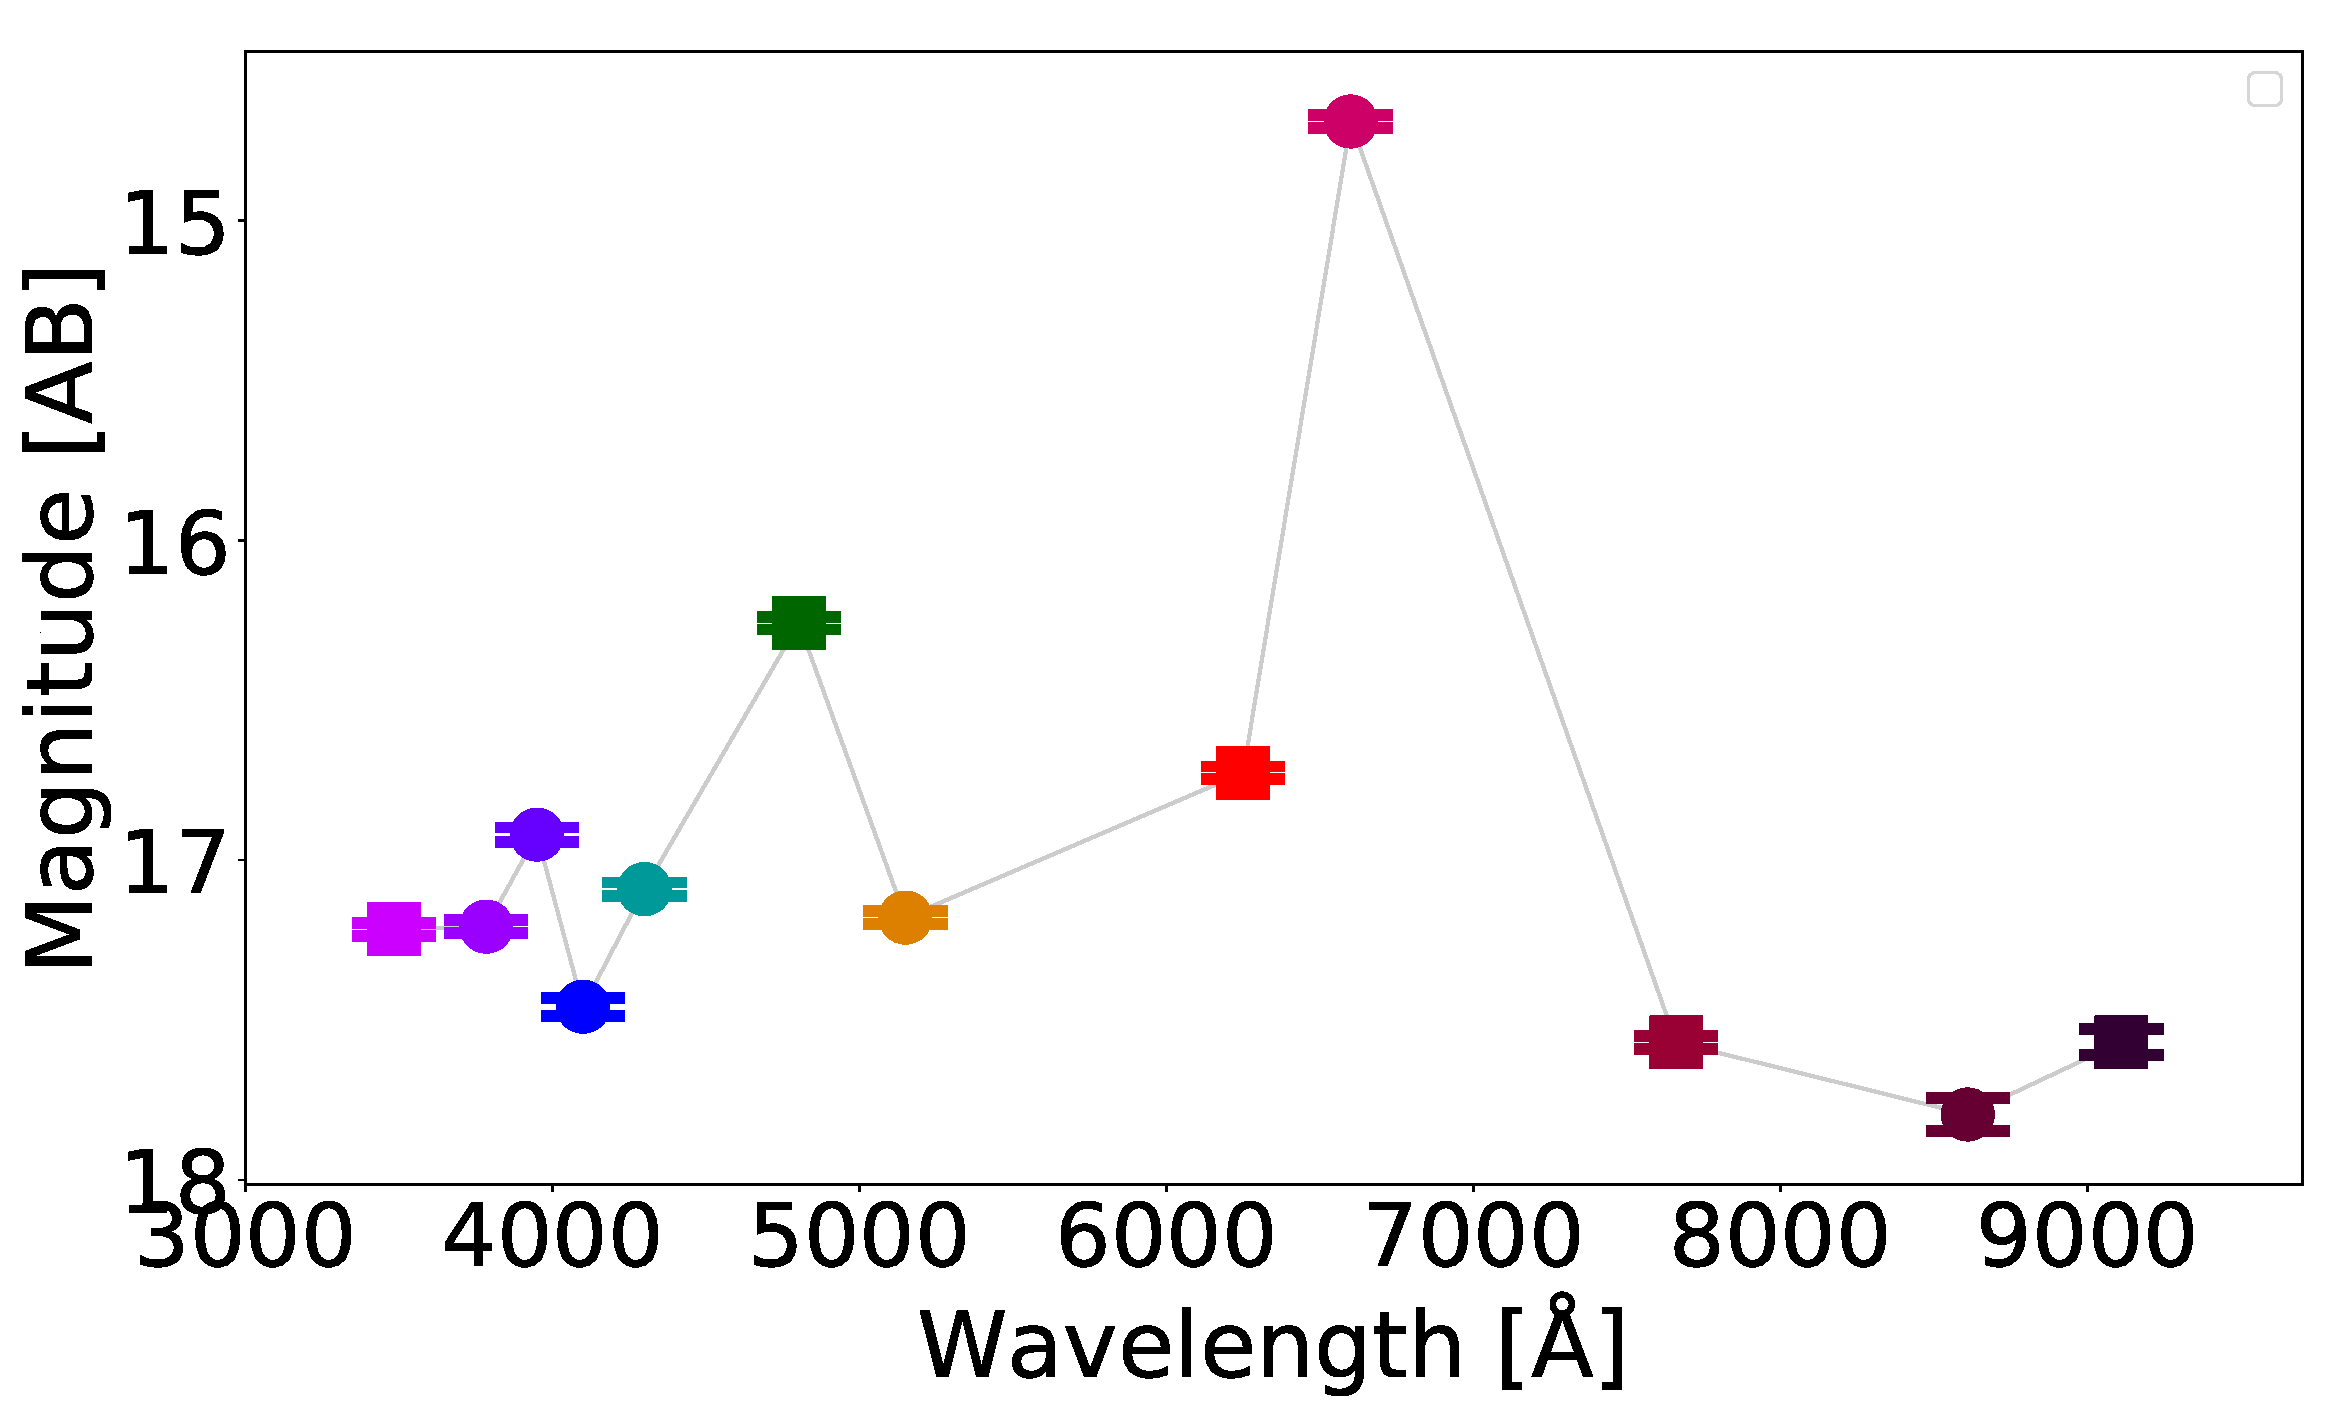
\includegraphics[width=0.3\linewidth, clip]{photopectrum_splus_MC0093-085620_auto.pdf} & 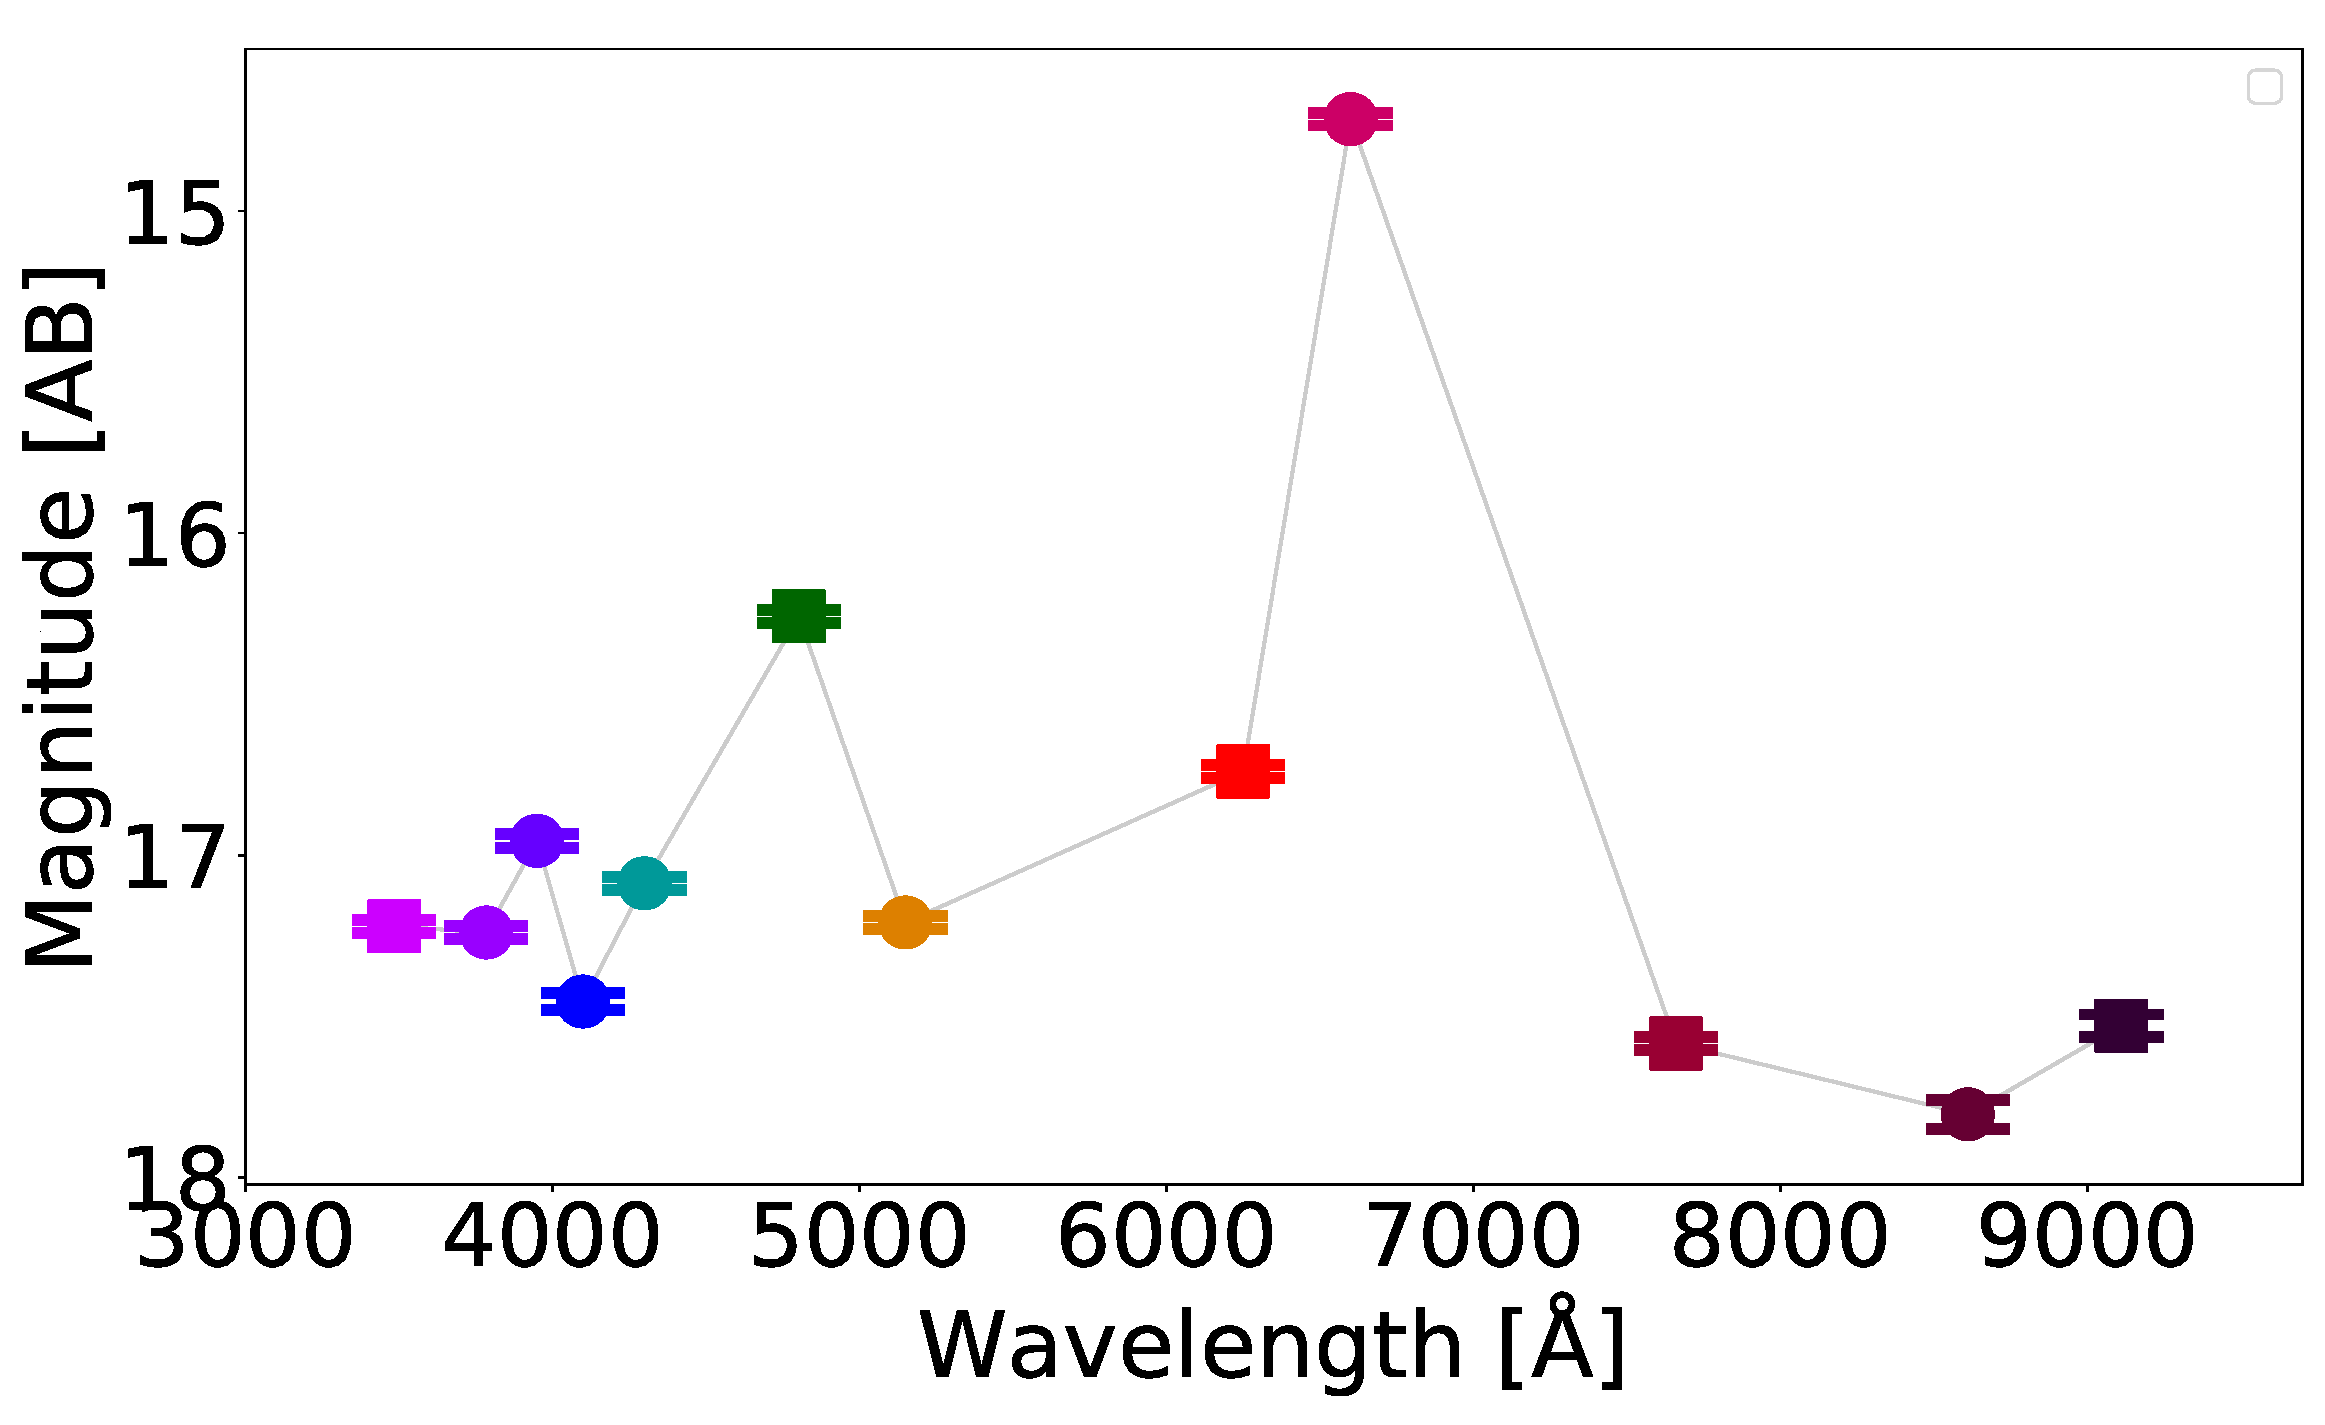
\includegraphics[width=0.3\linewidth, clip]{photopectrum_splus_MC0093-085620_petro.pdf} \\
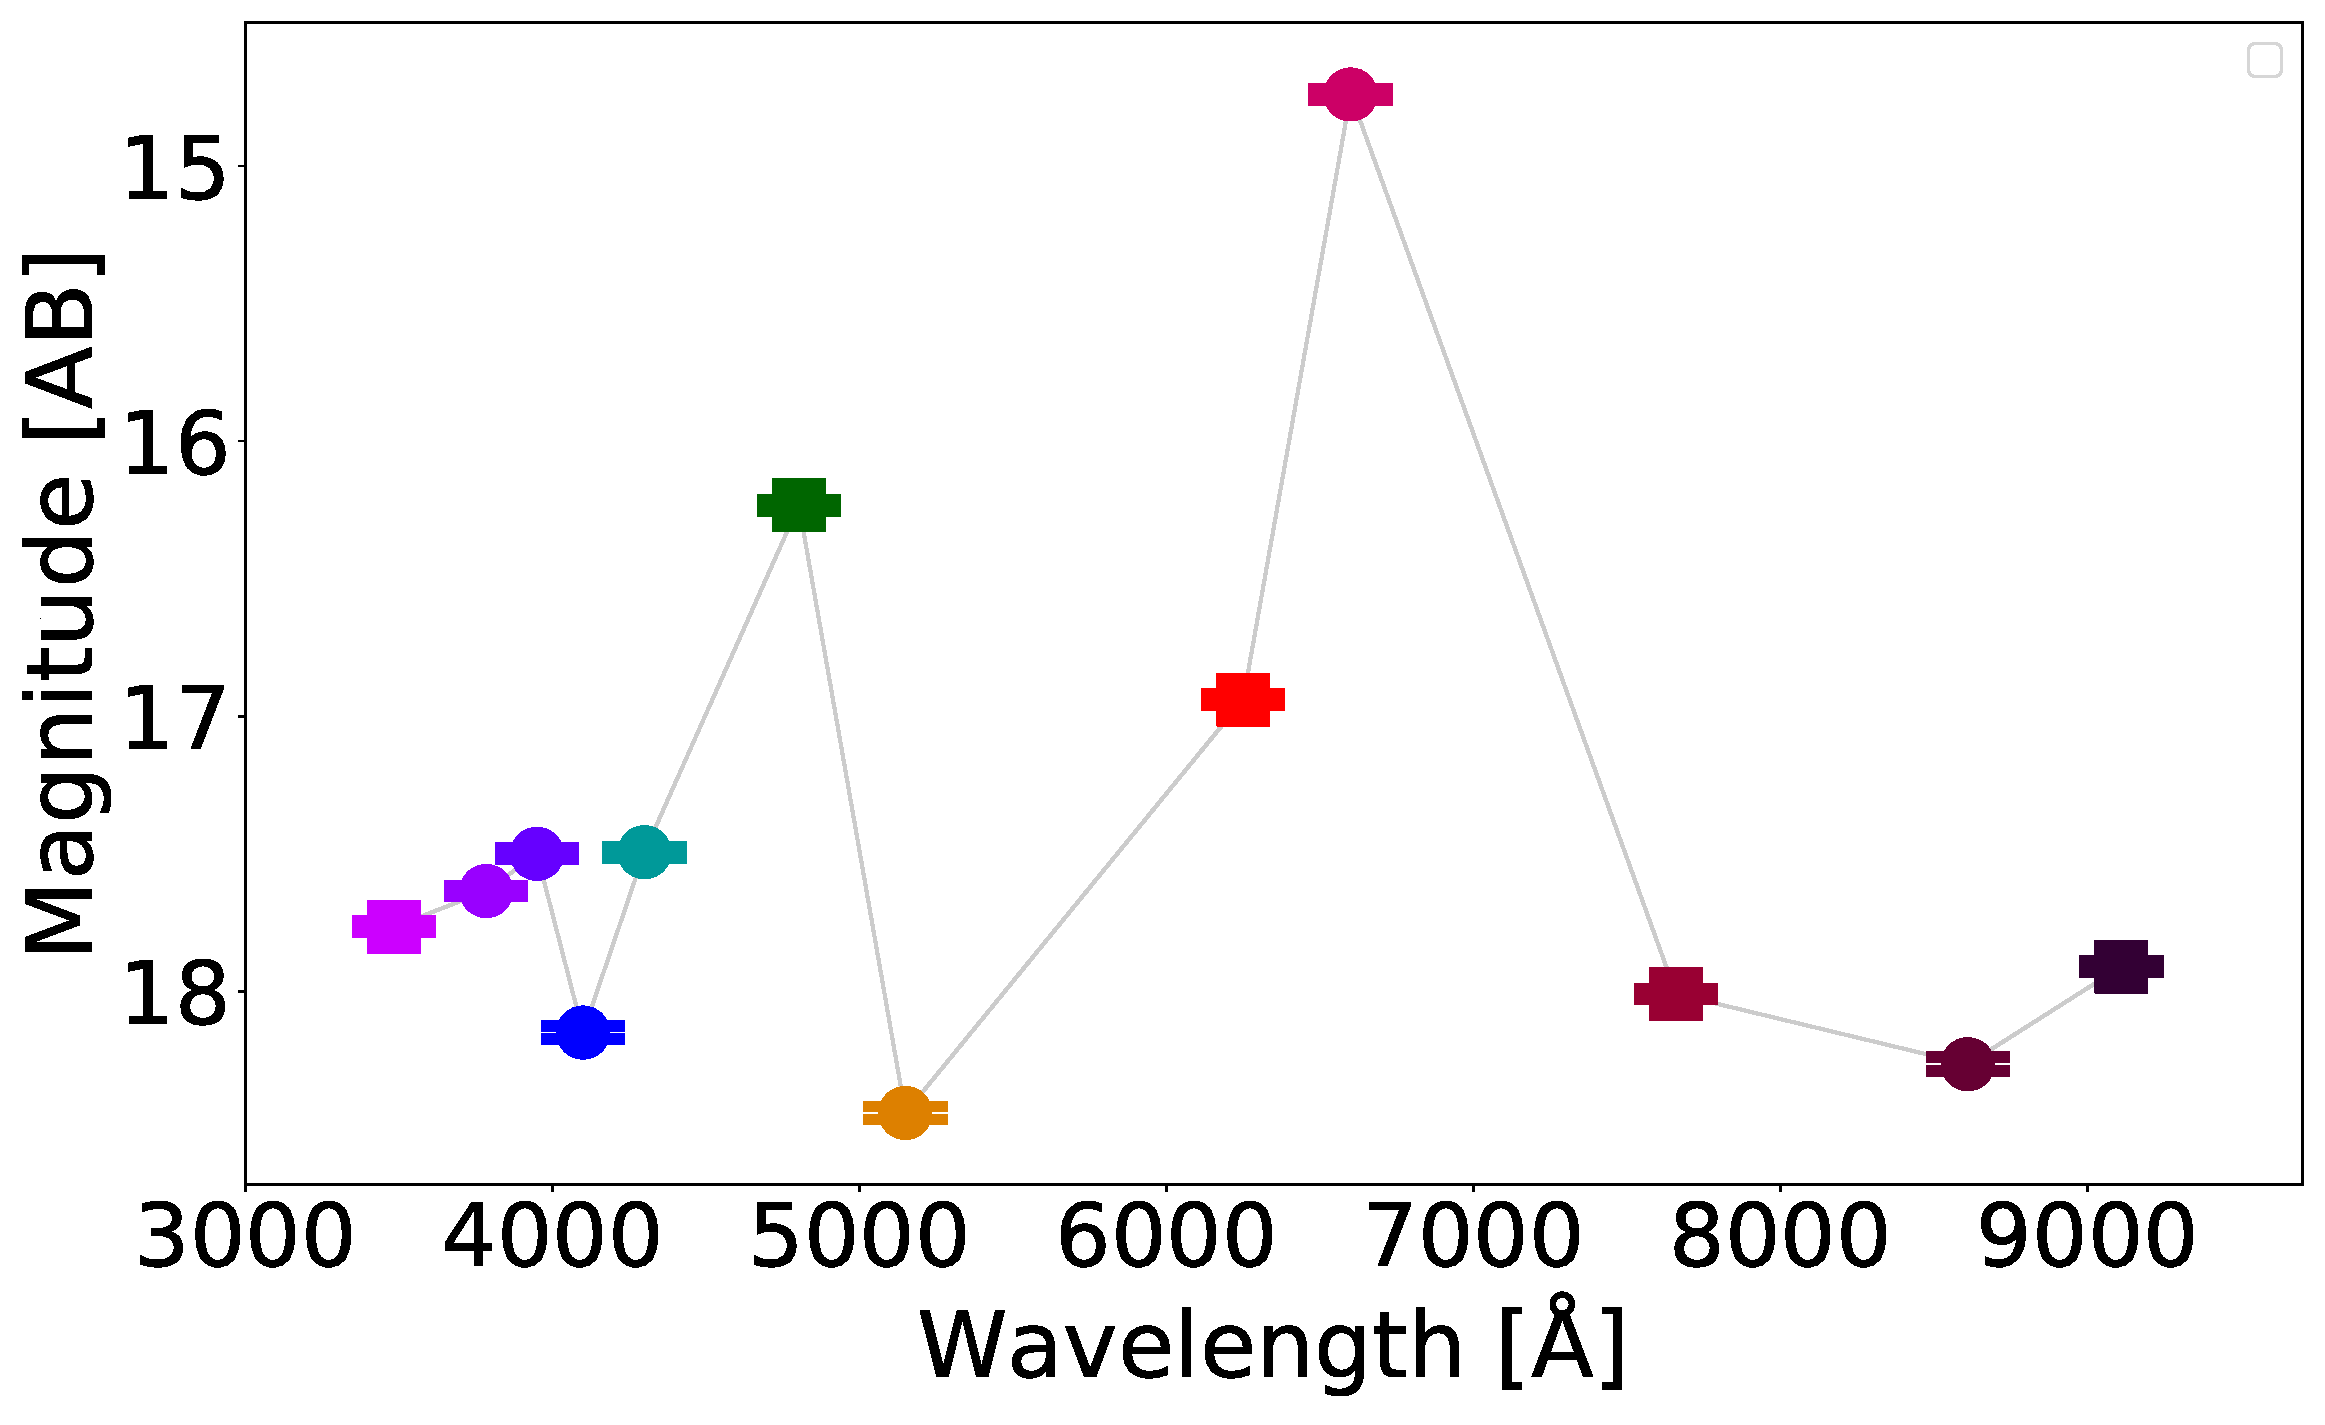
\includegraphics[width=0.3\linewidth, clip]{photopectrum_splus_MC0093-295870_aper.pdf} & 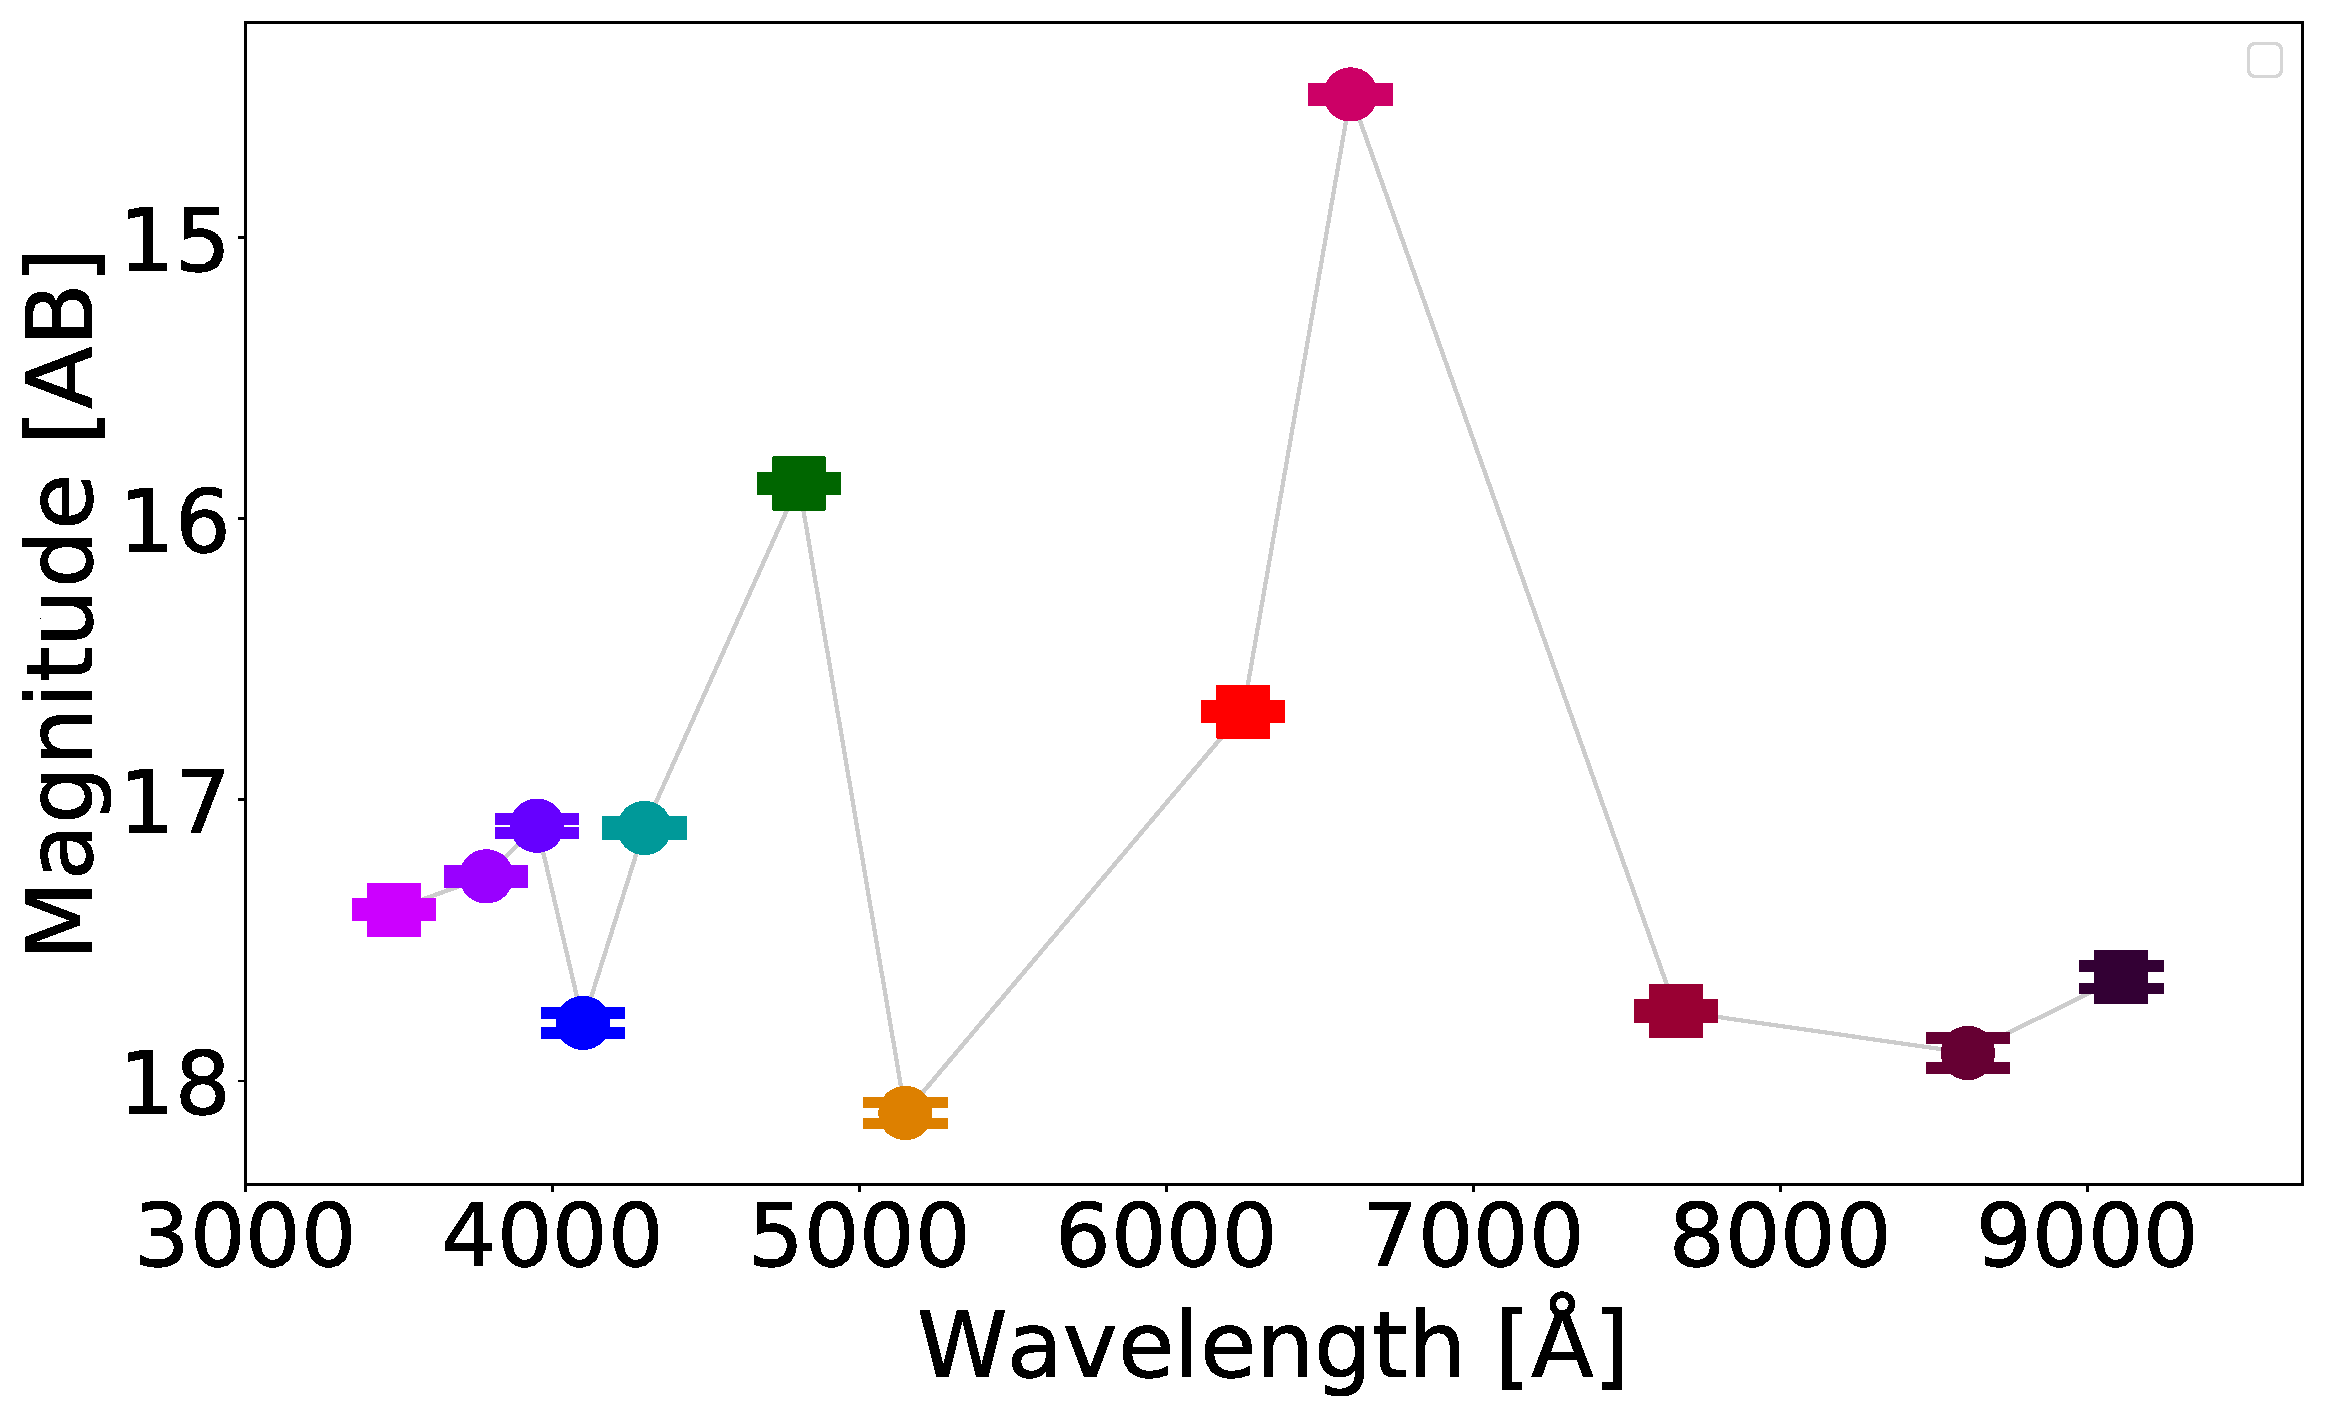
\includegraphics[width=0.3\linewidth, clip]{photopectrum_splus_MC0093-295870_auto.pdf} & 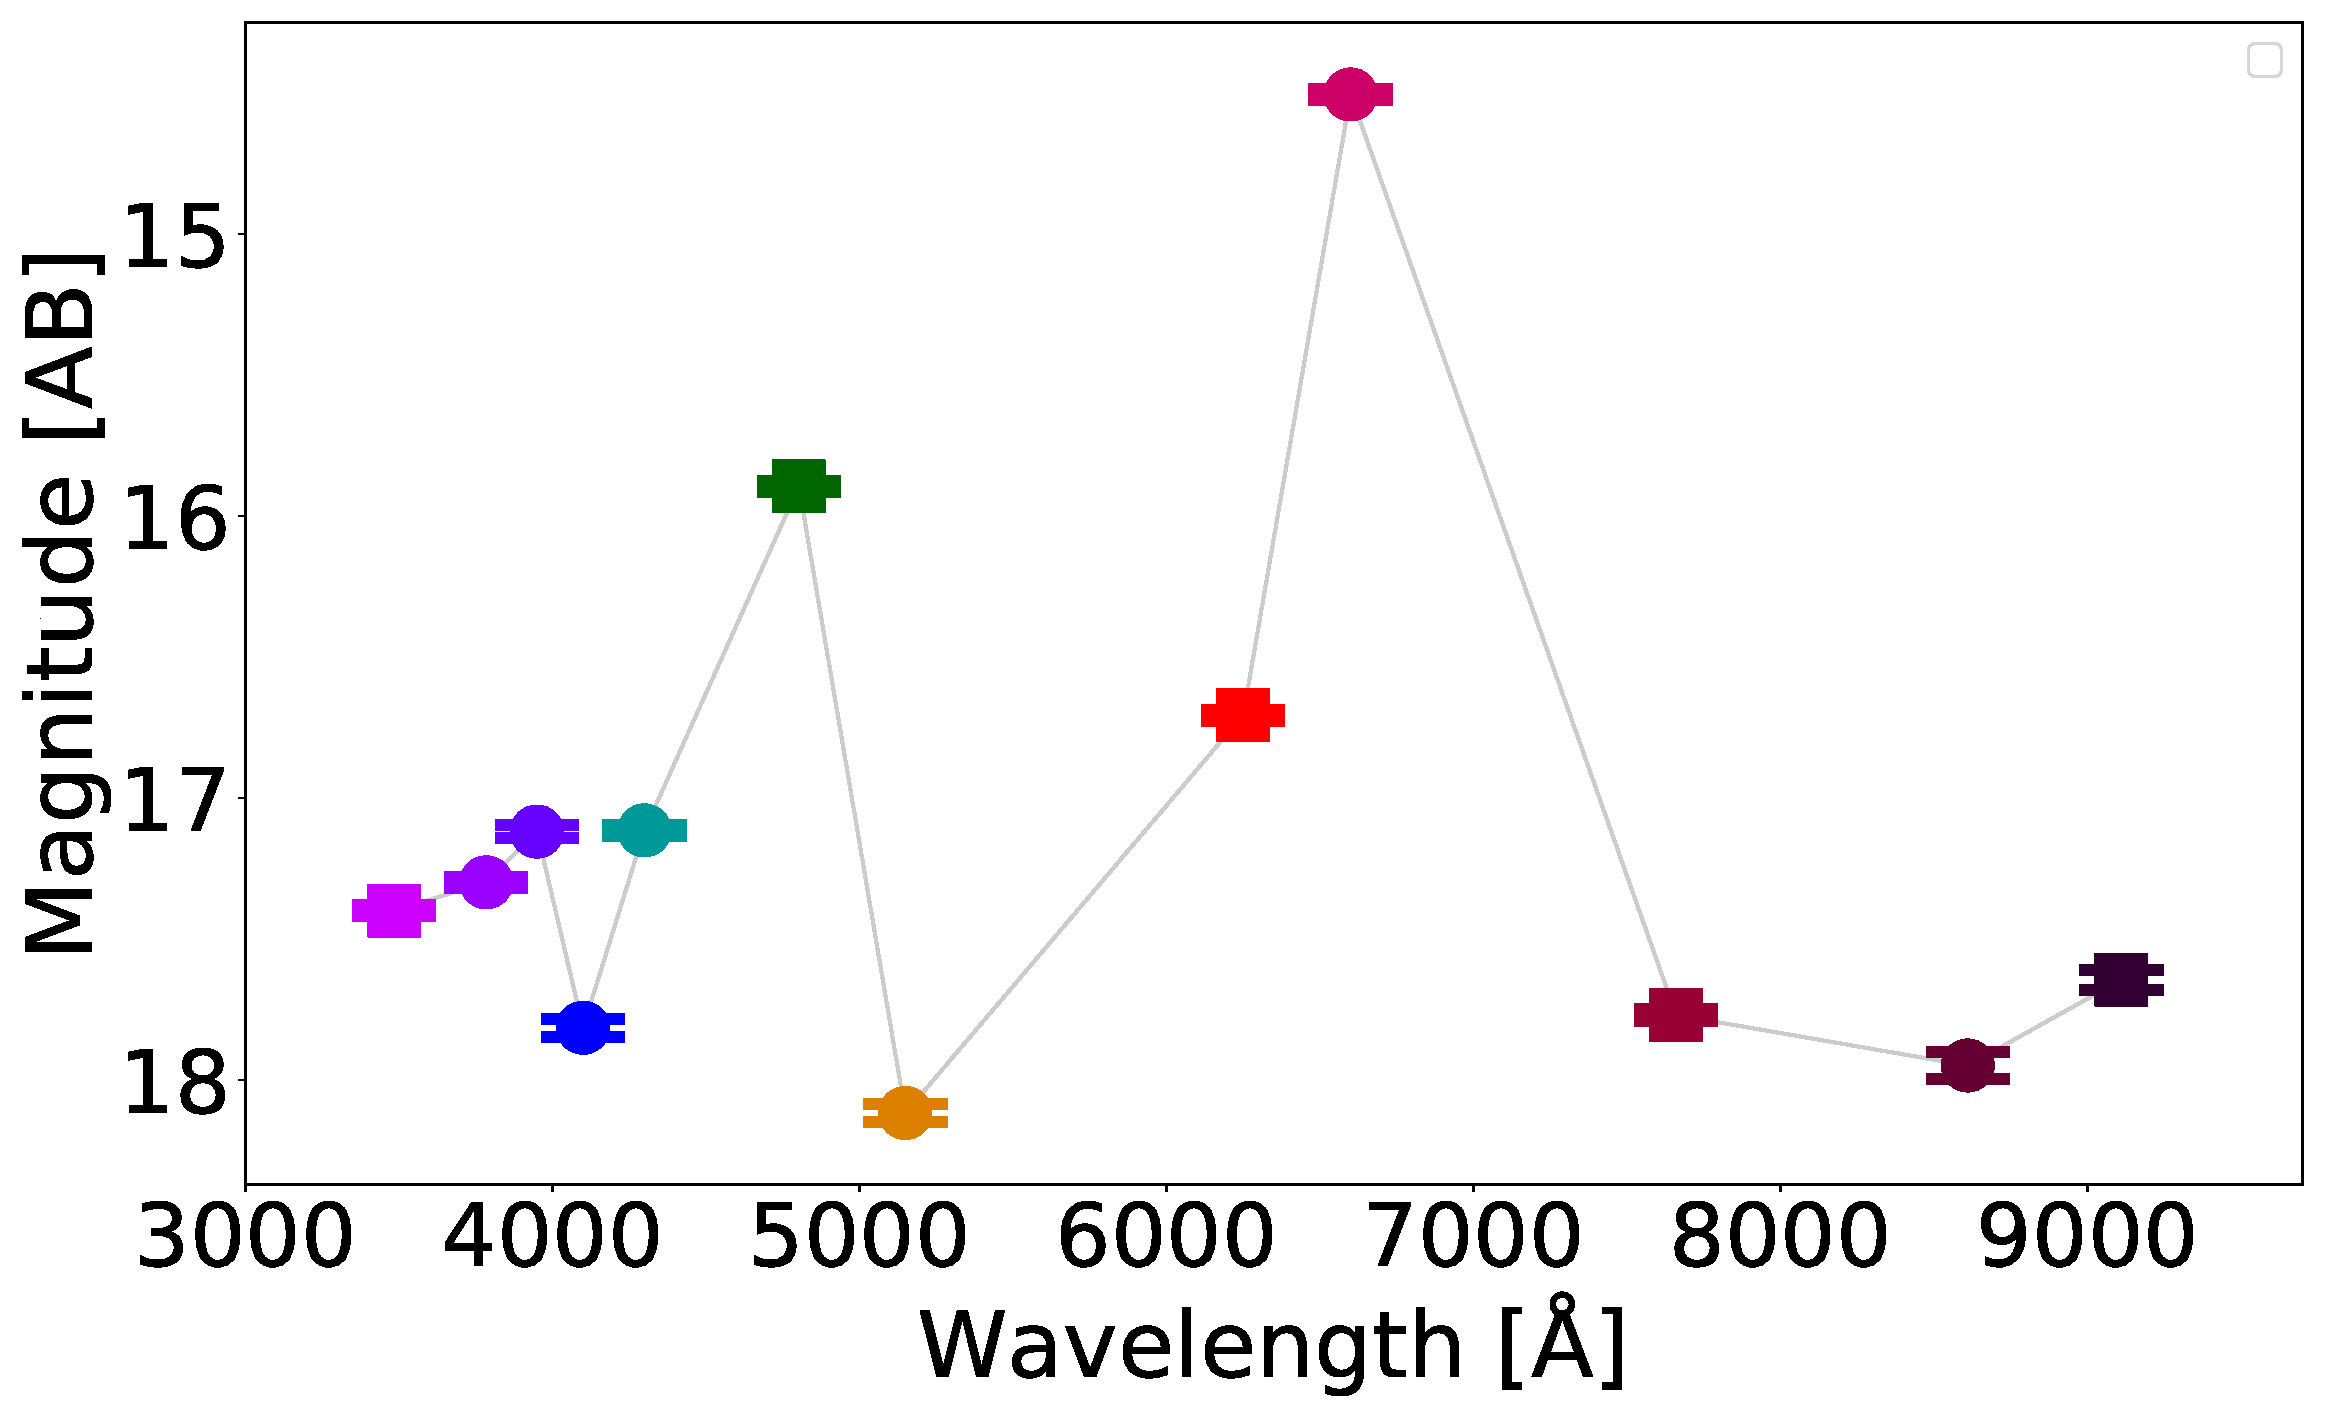
\includegraphics[width=0.3\linewidth, clip]{photopectrum_splus_MC0093-295870_petro.pdf} \\
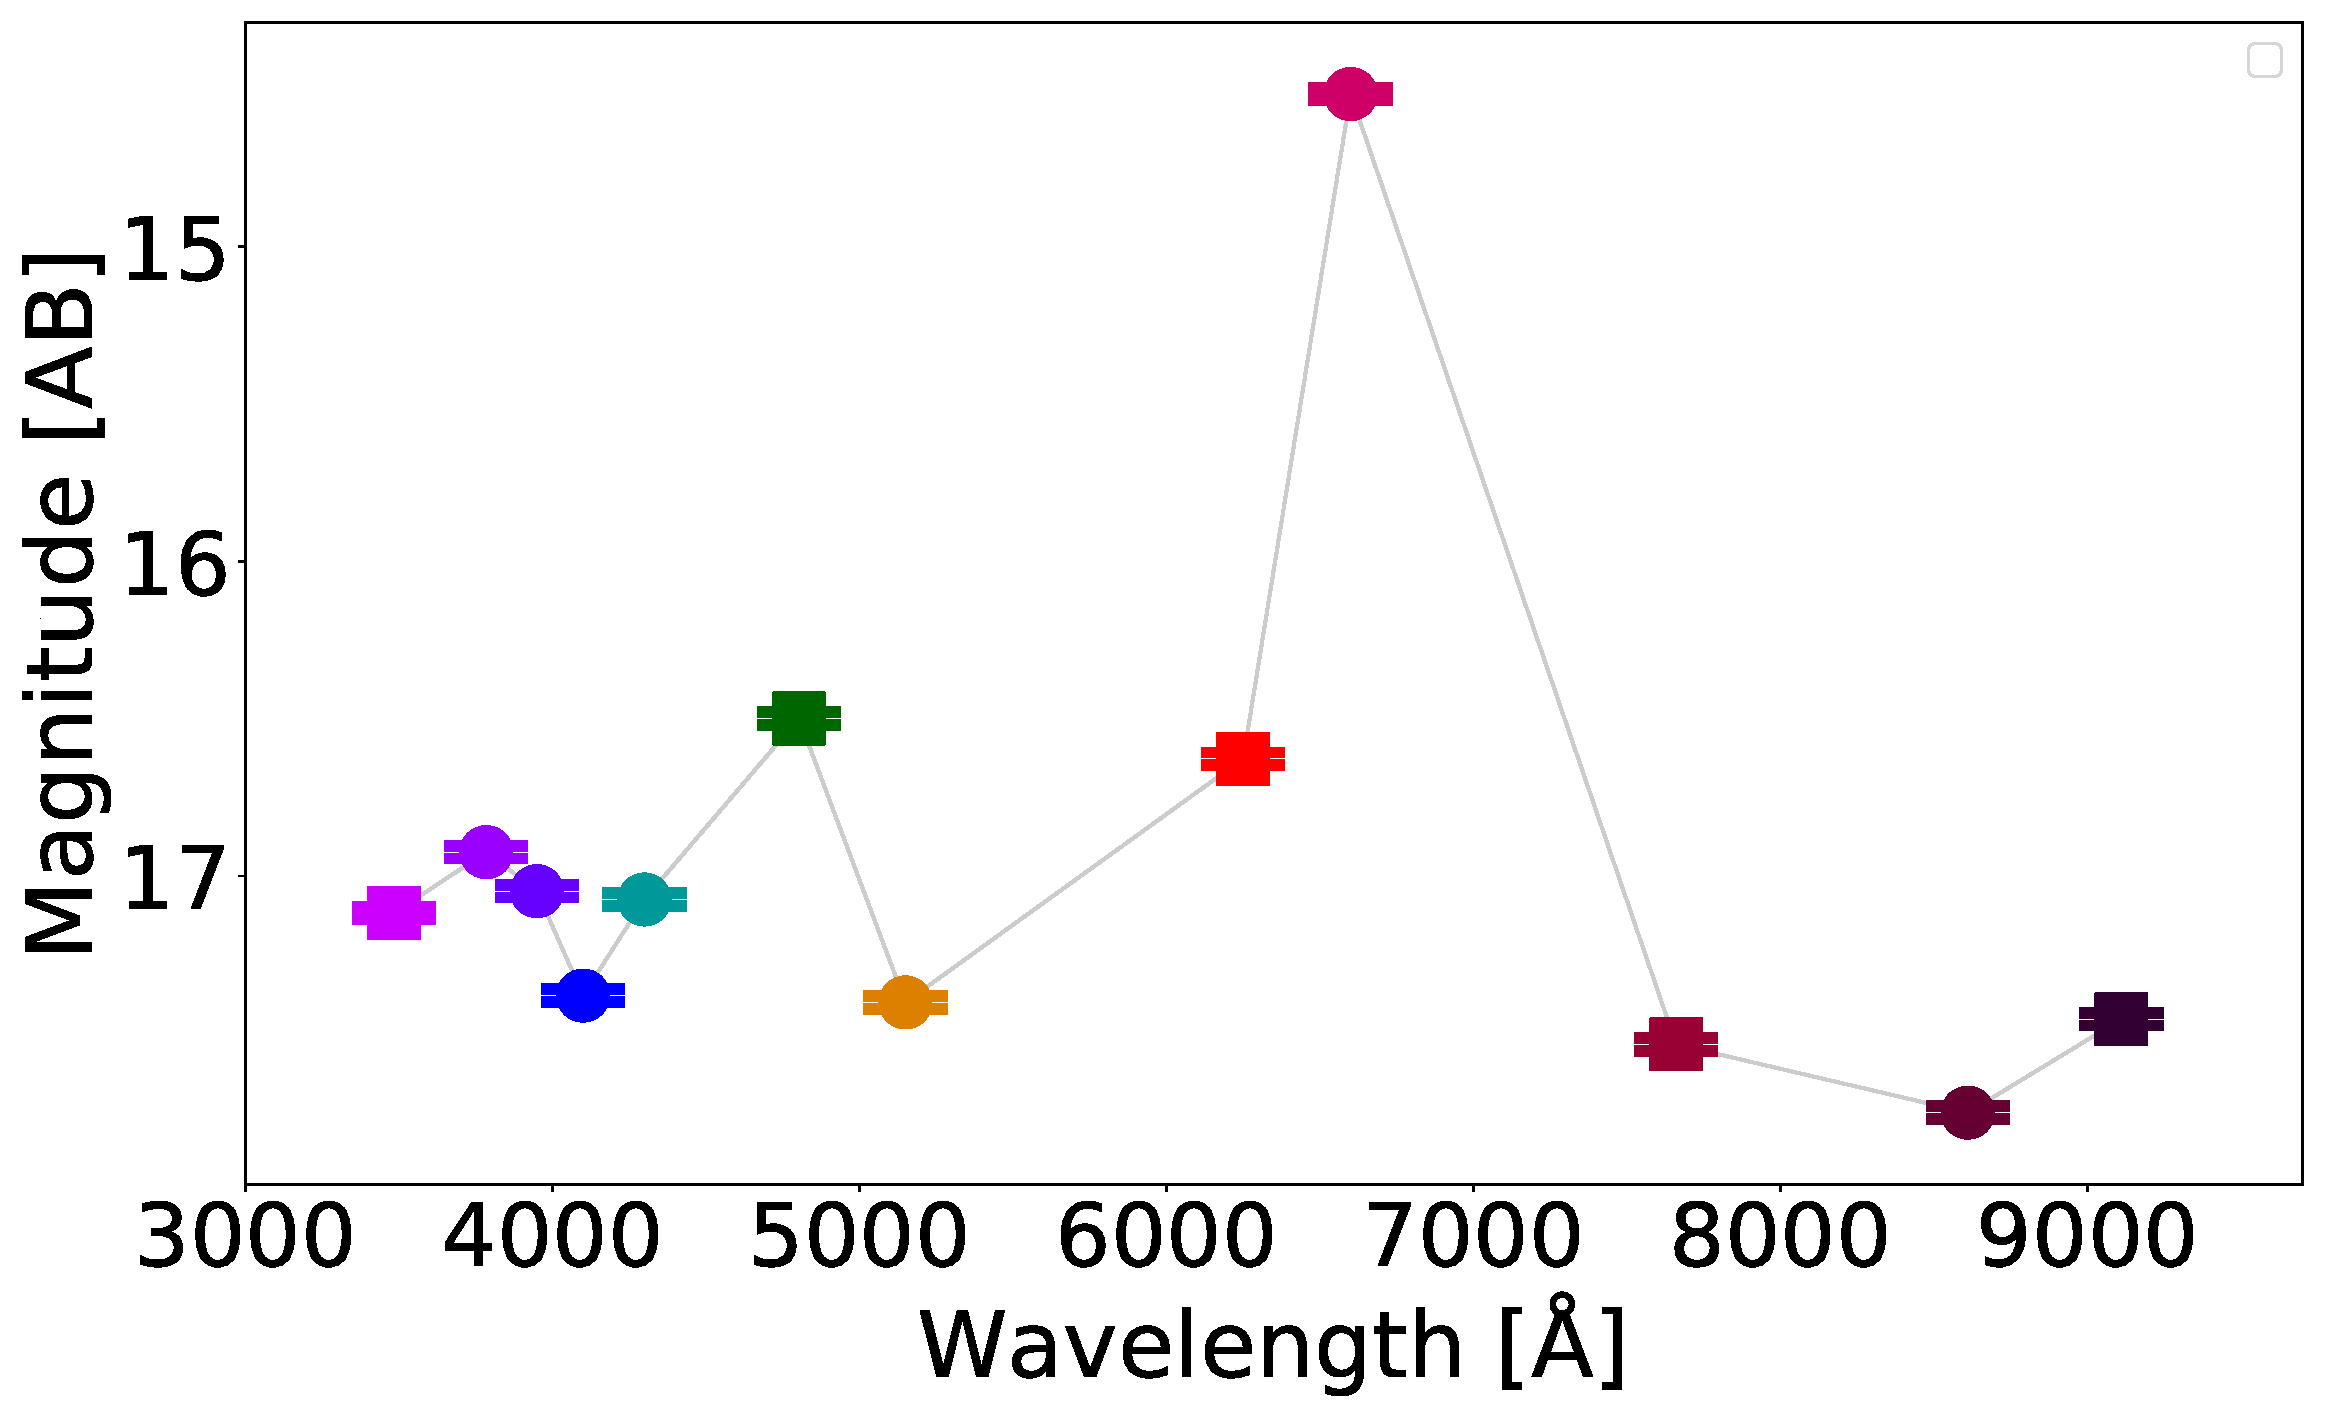
\includegraphics[width=0.3\linewidth, clip]{photopectrum_splus_MC0094-194143_aper.pdf} & 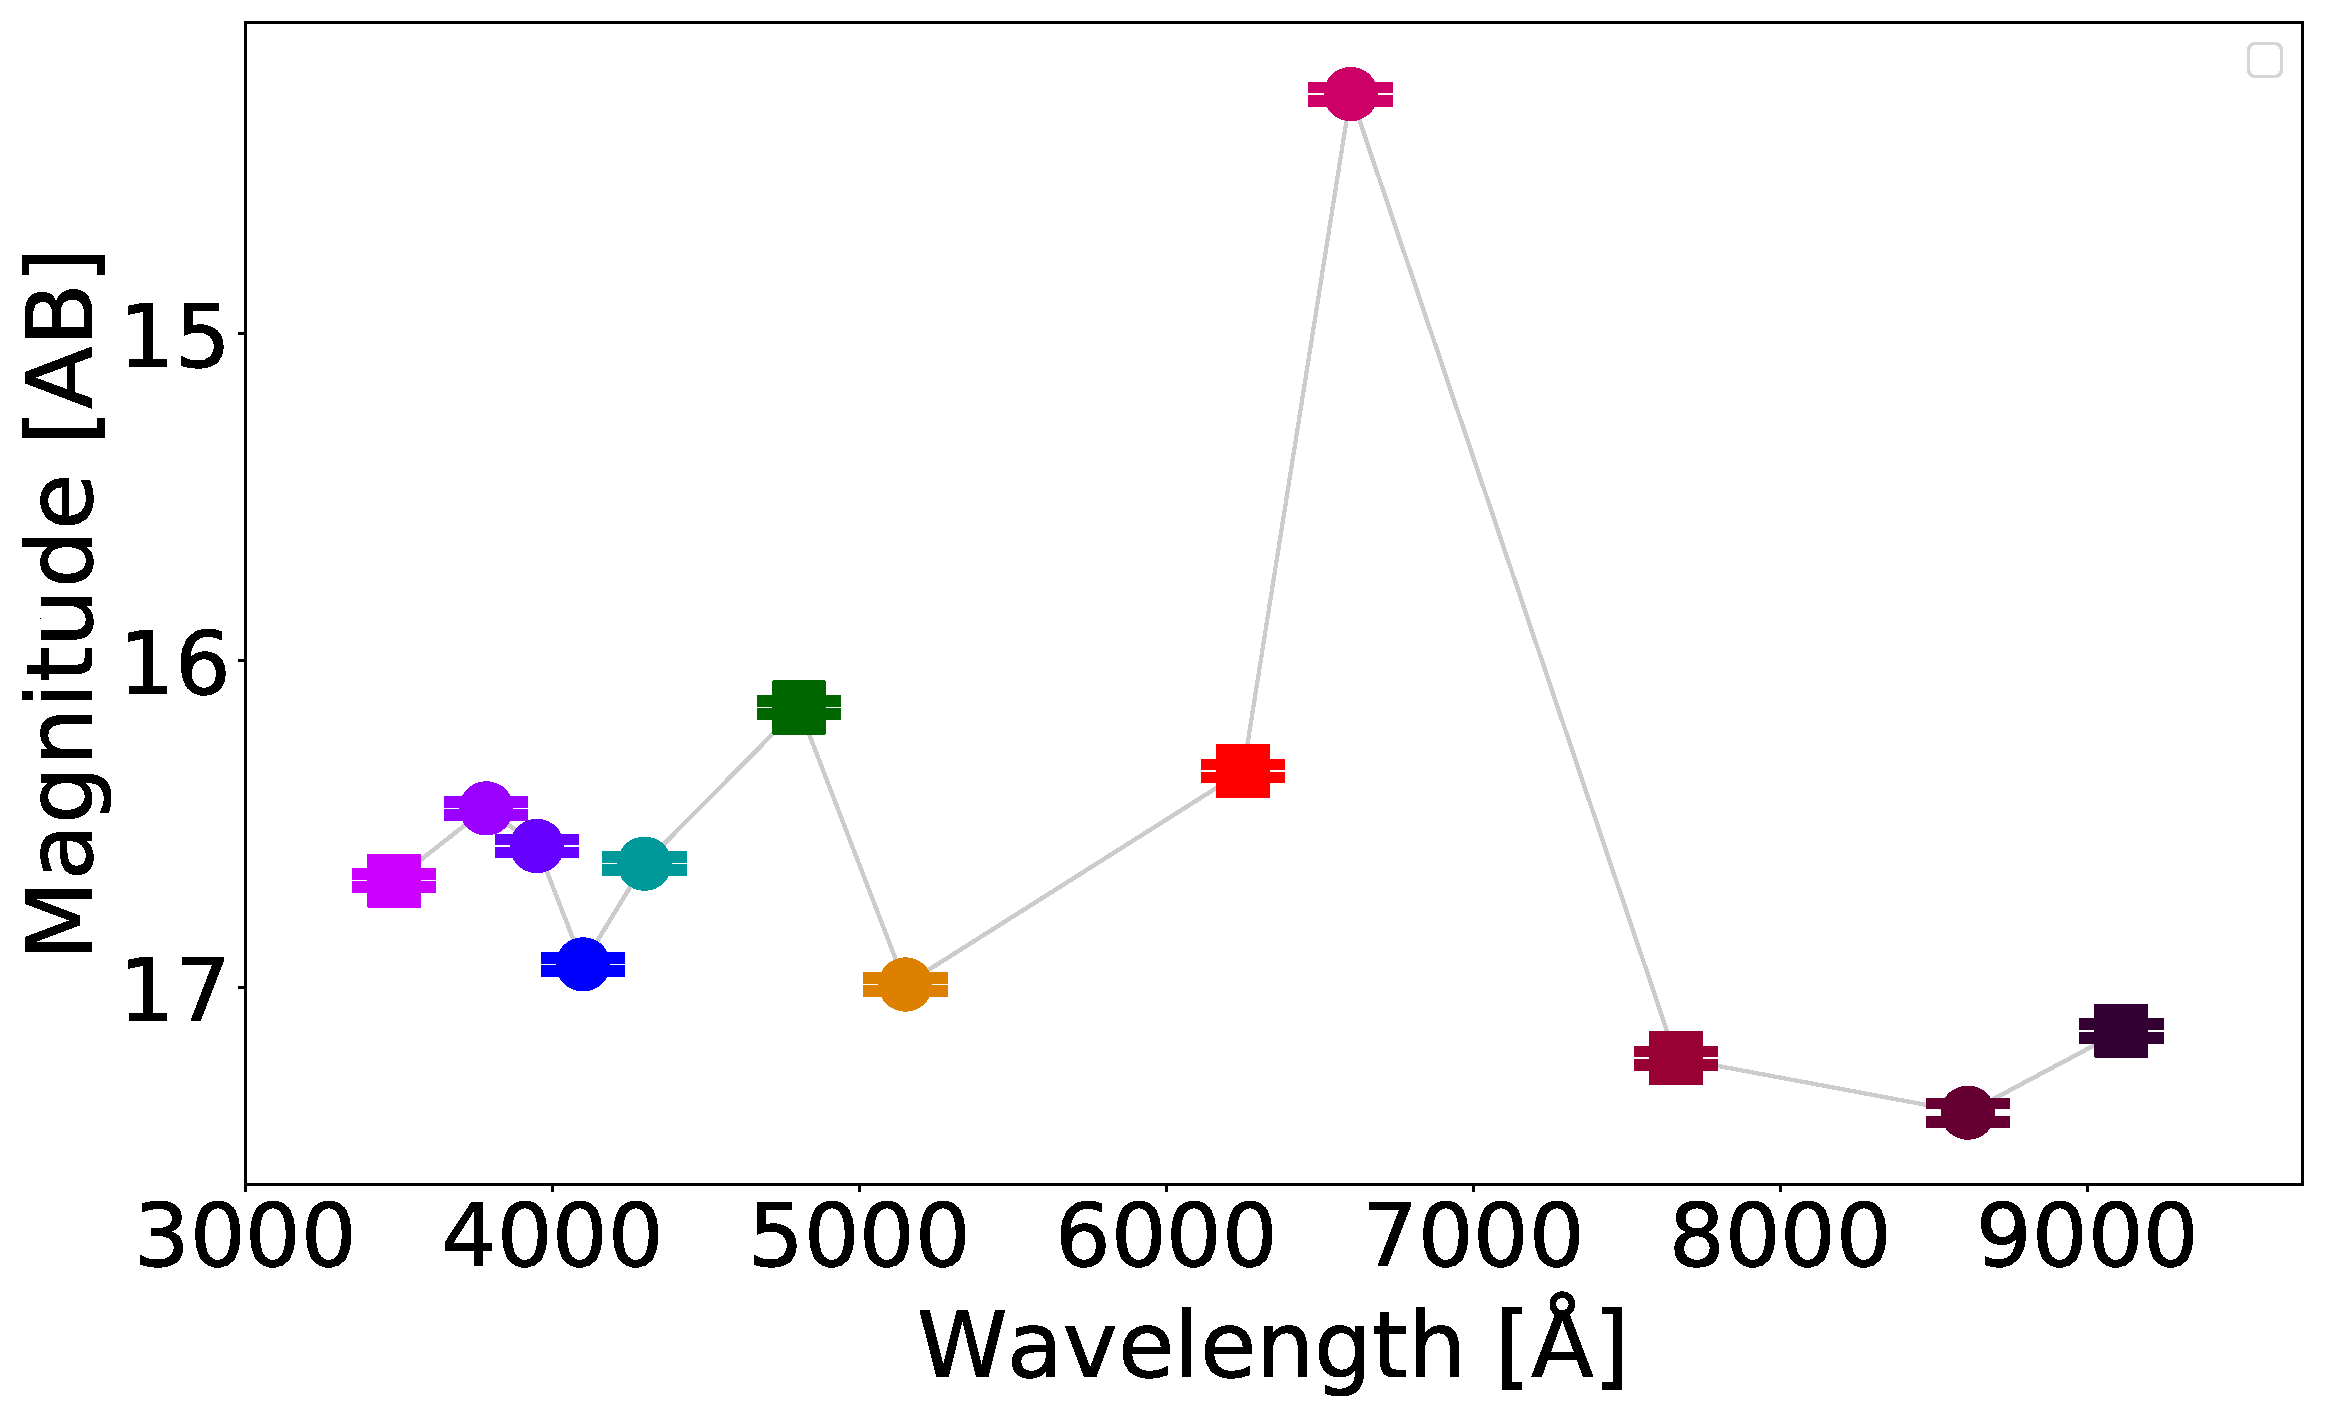
\includegraphics[width=0.3\linewidth, clip]{photopectrum_splus_MC0094-194143_auto.pdf} & 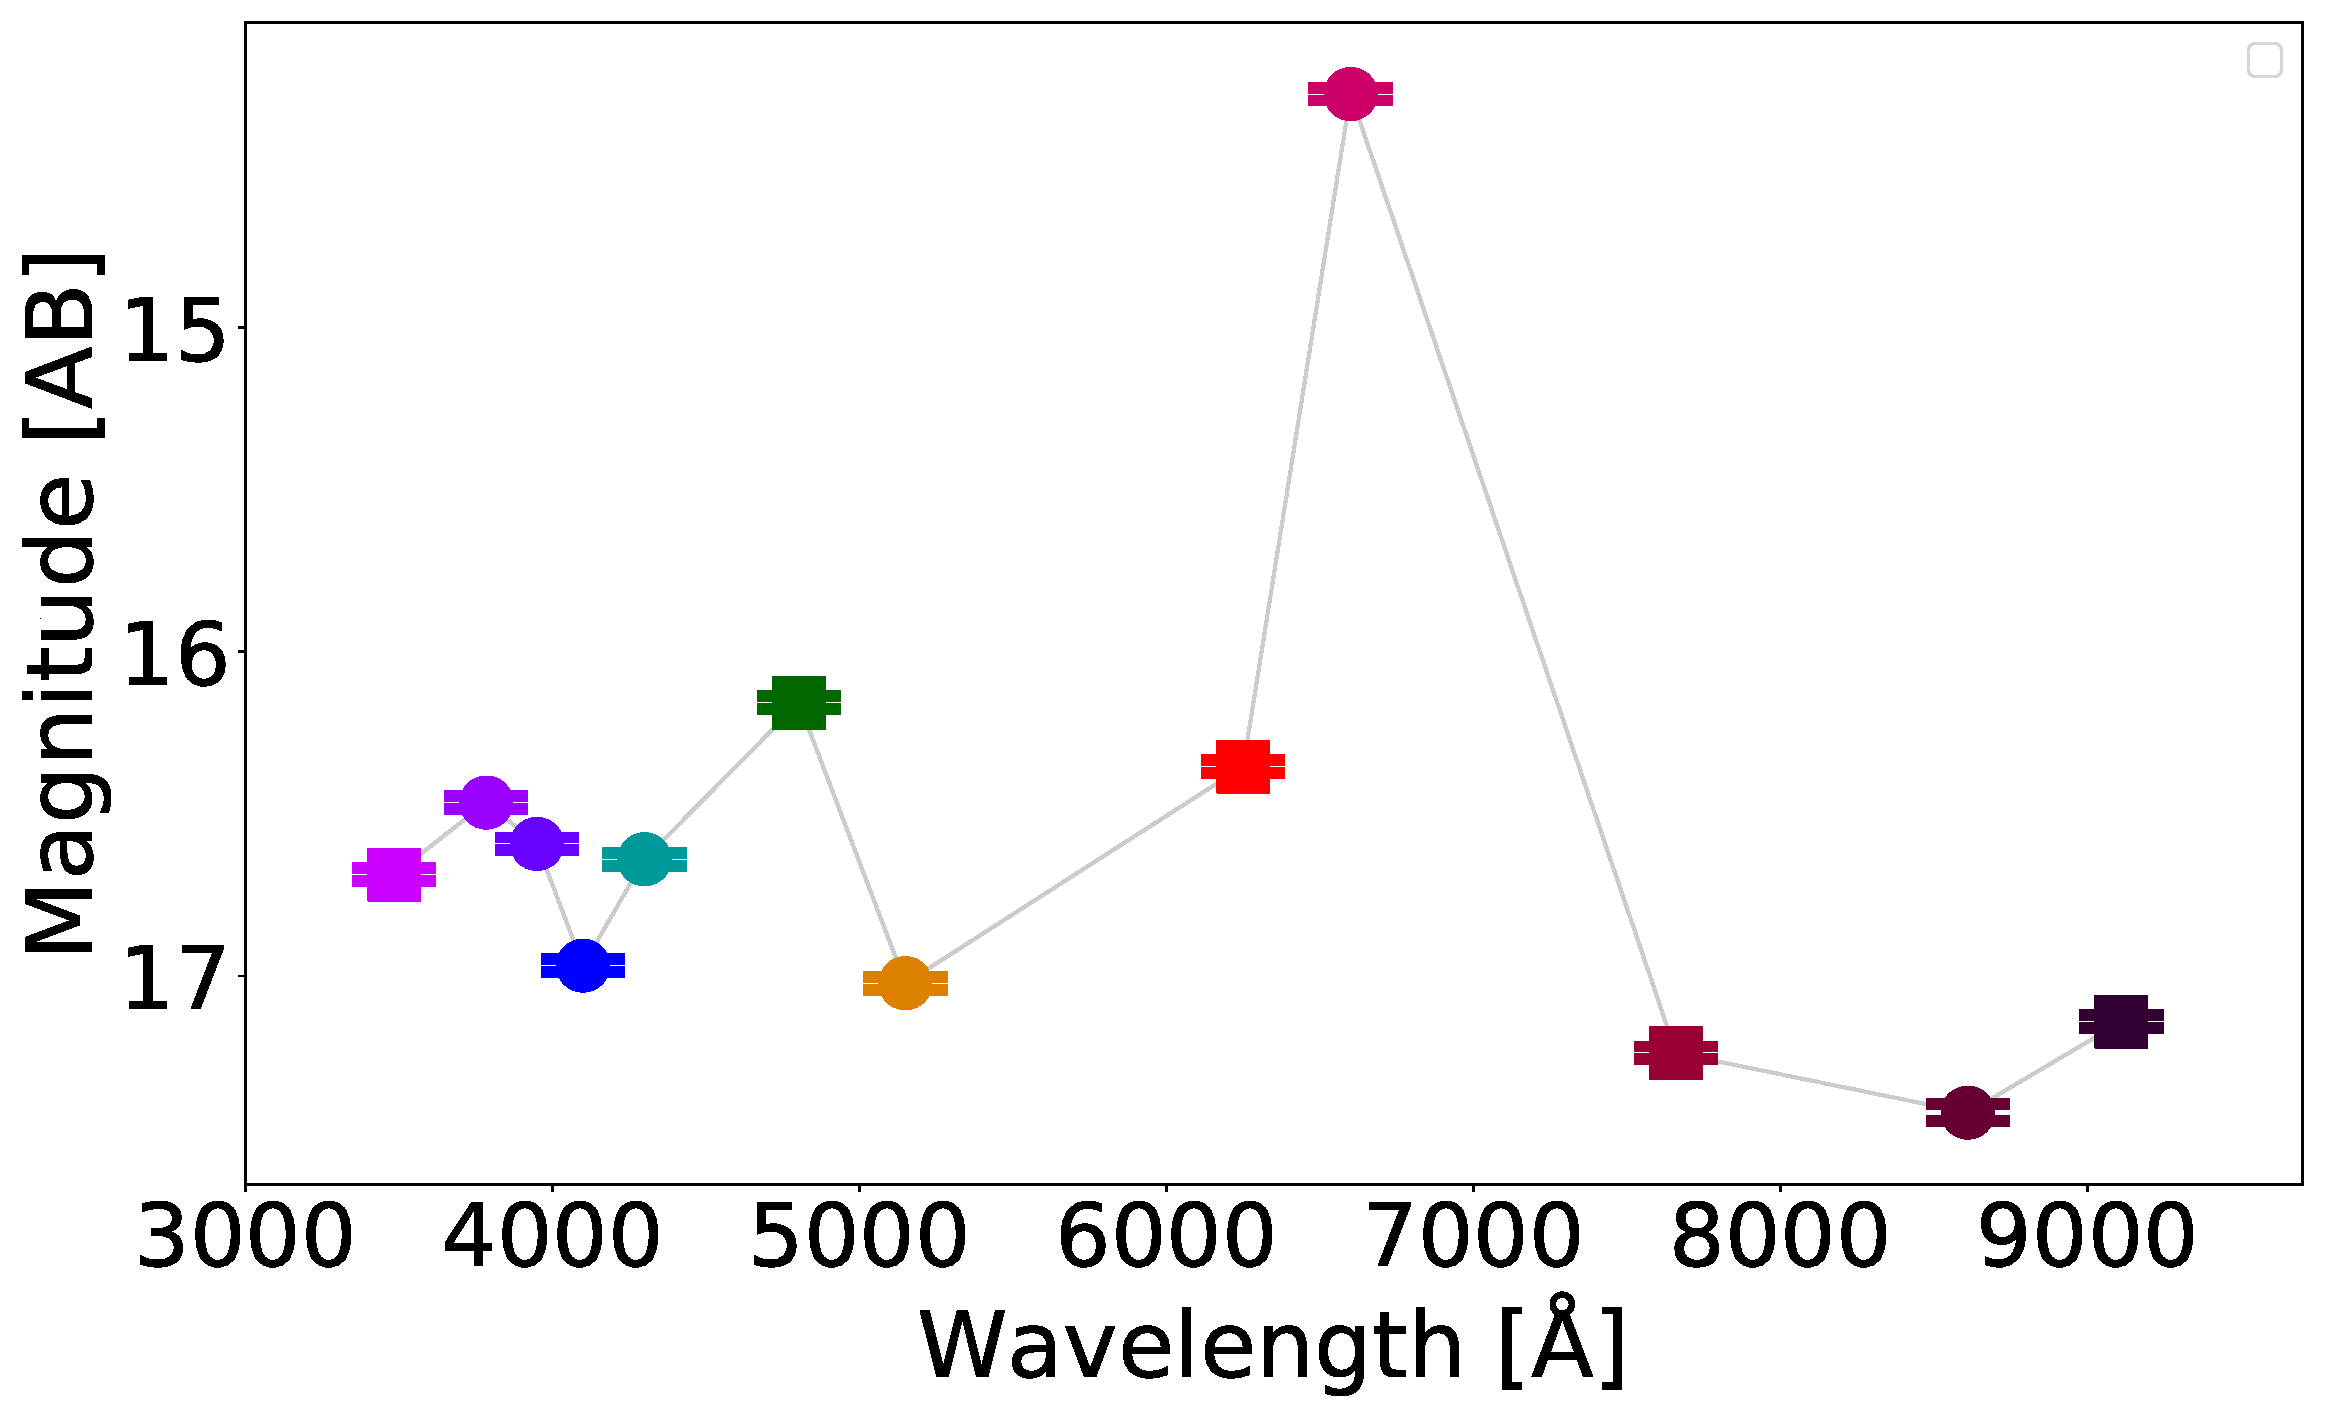
\includegraphics[width=0.3\linewidth, clip]{photopectrum_splus_MC0094-194143_petro.pdf} \\
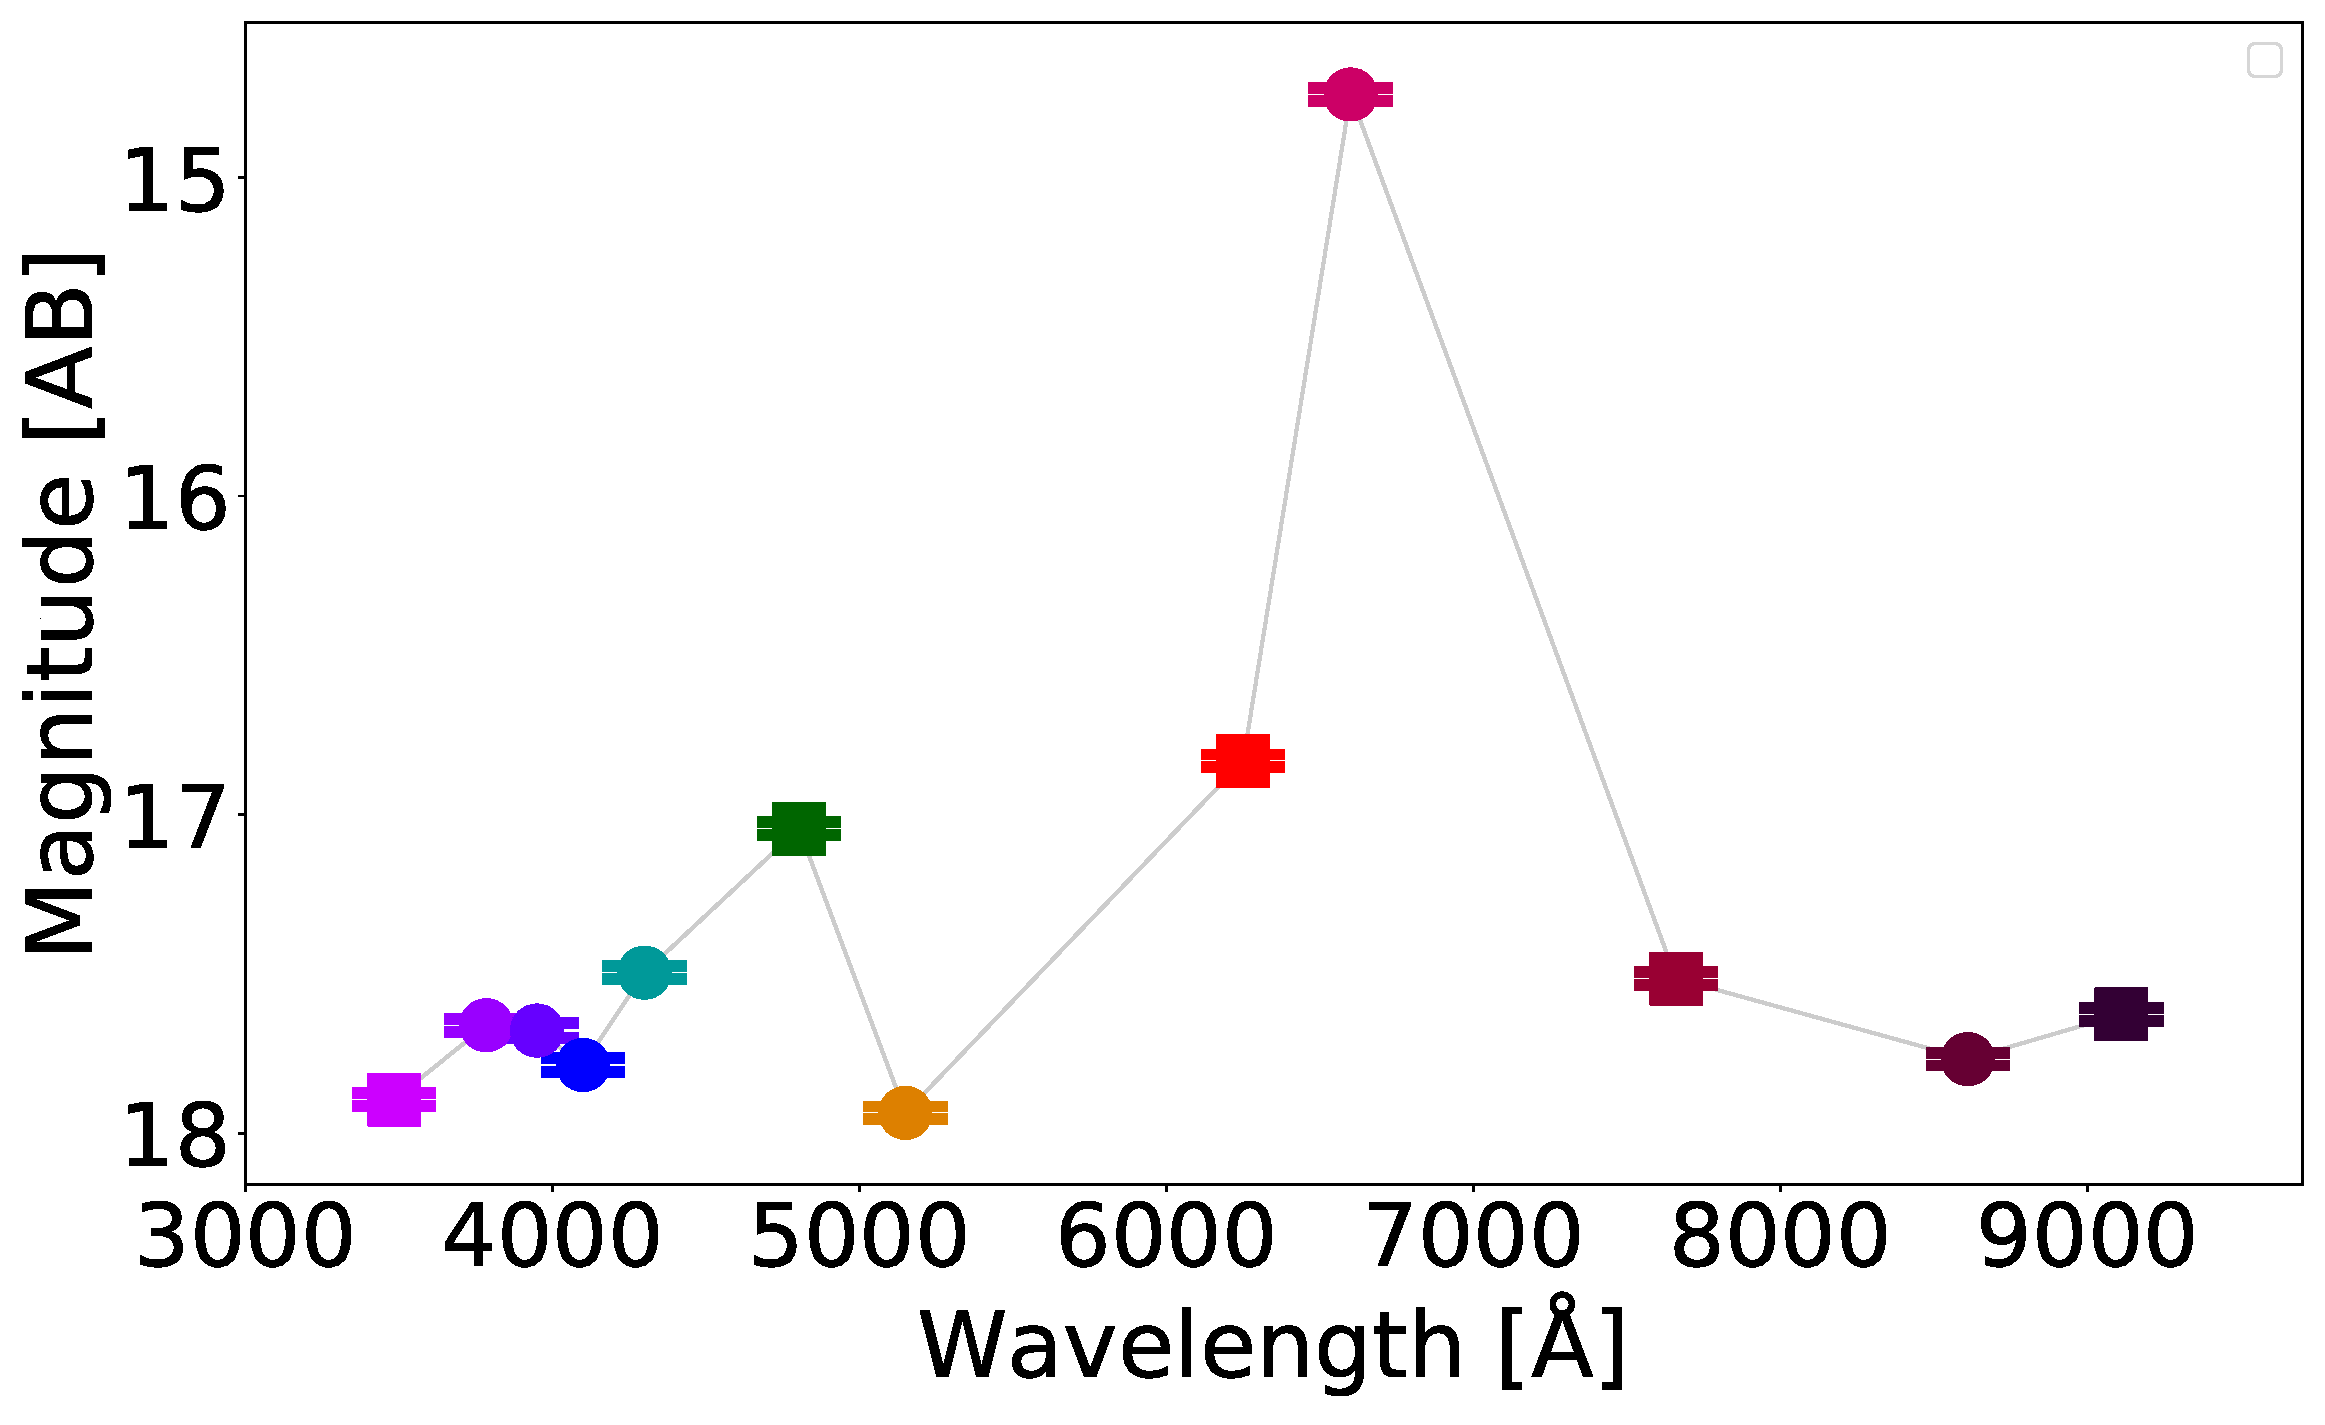
\includegraphics[width=0.3\linewidth, clip]{photopectrum_splus_MC0113-084466_aper.pdf} & 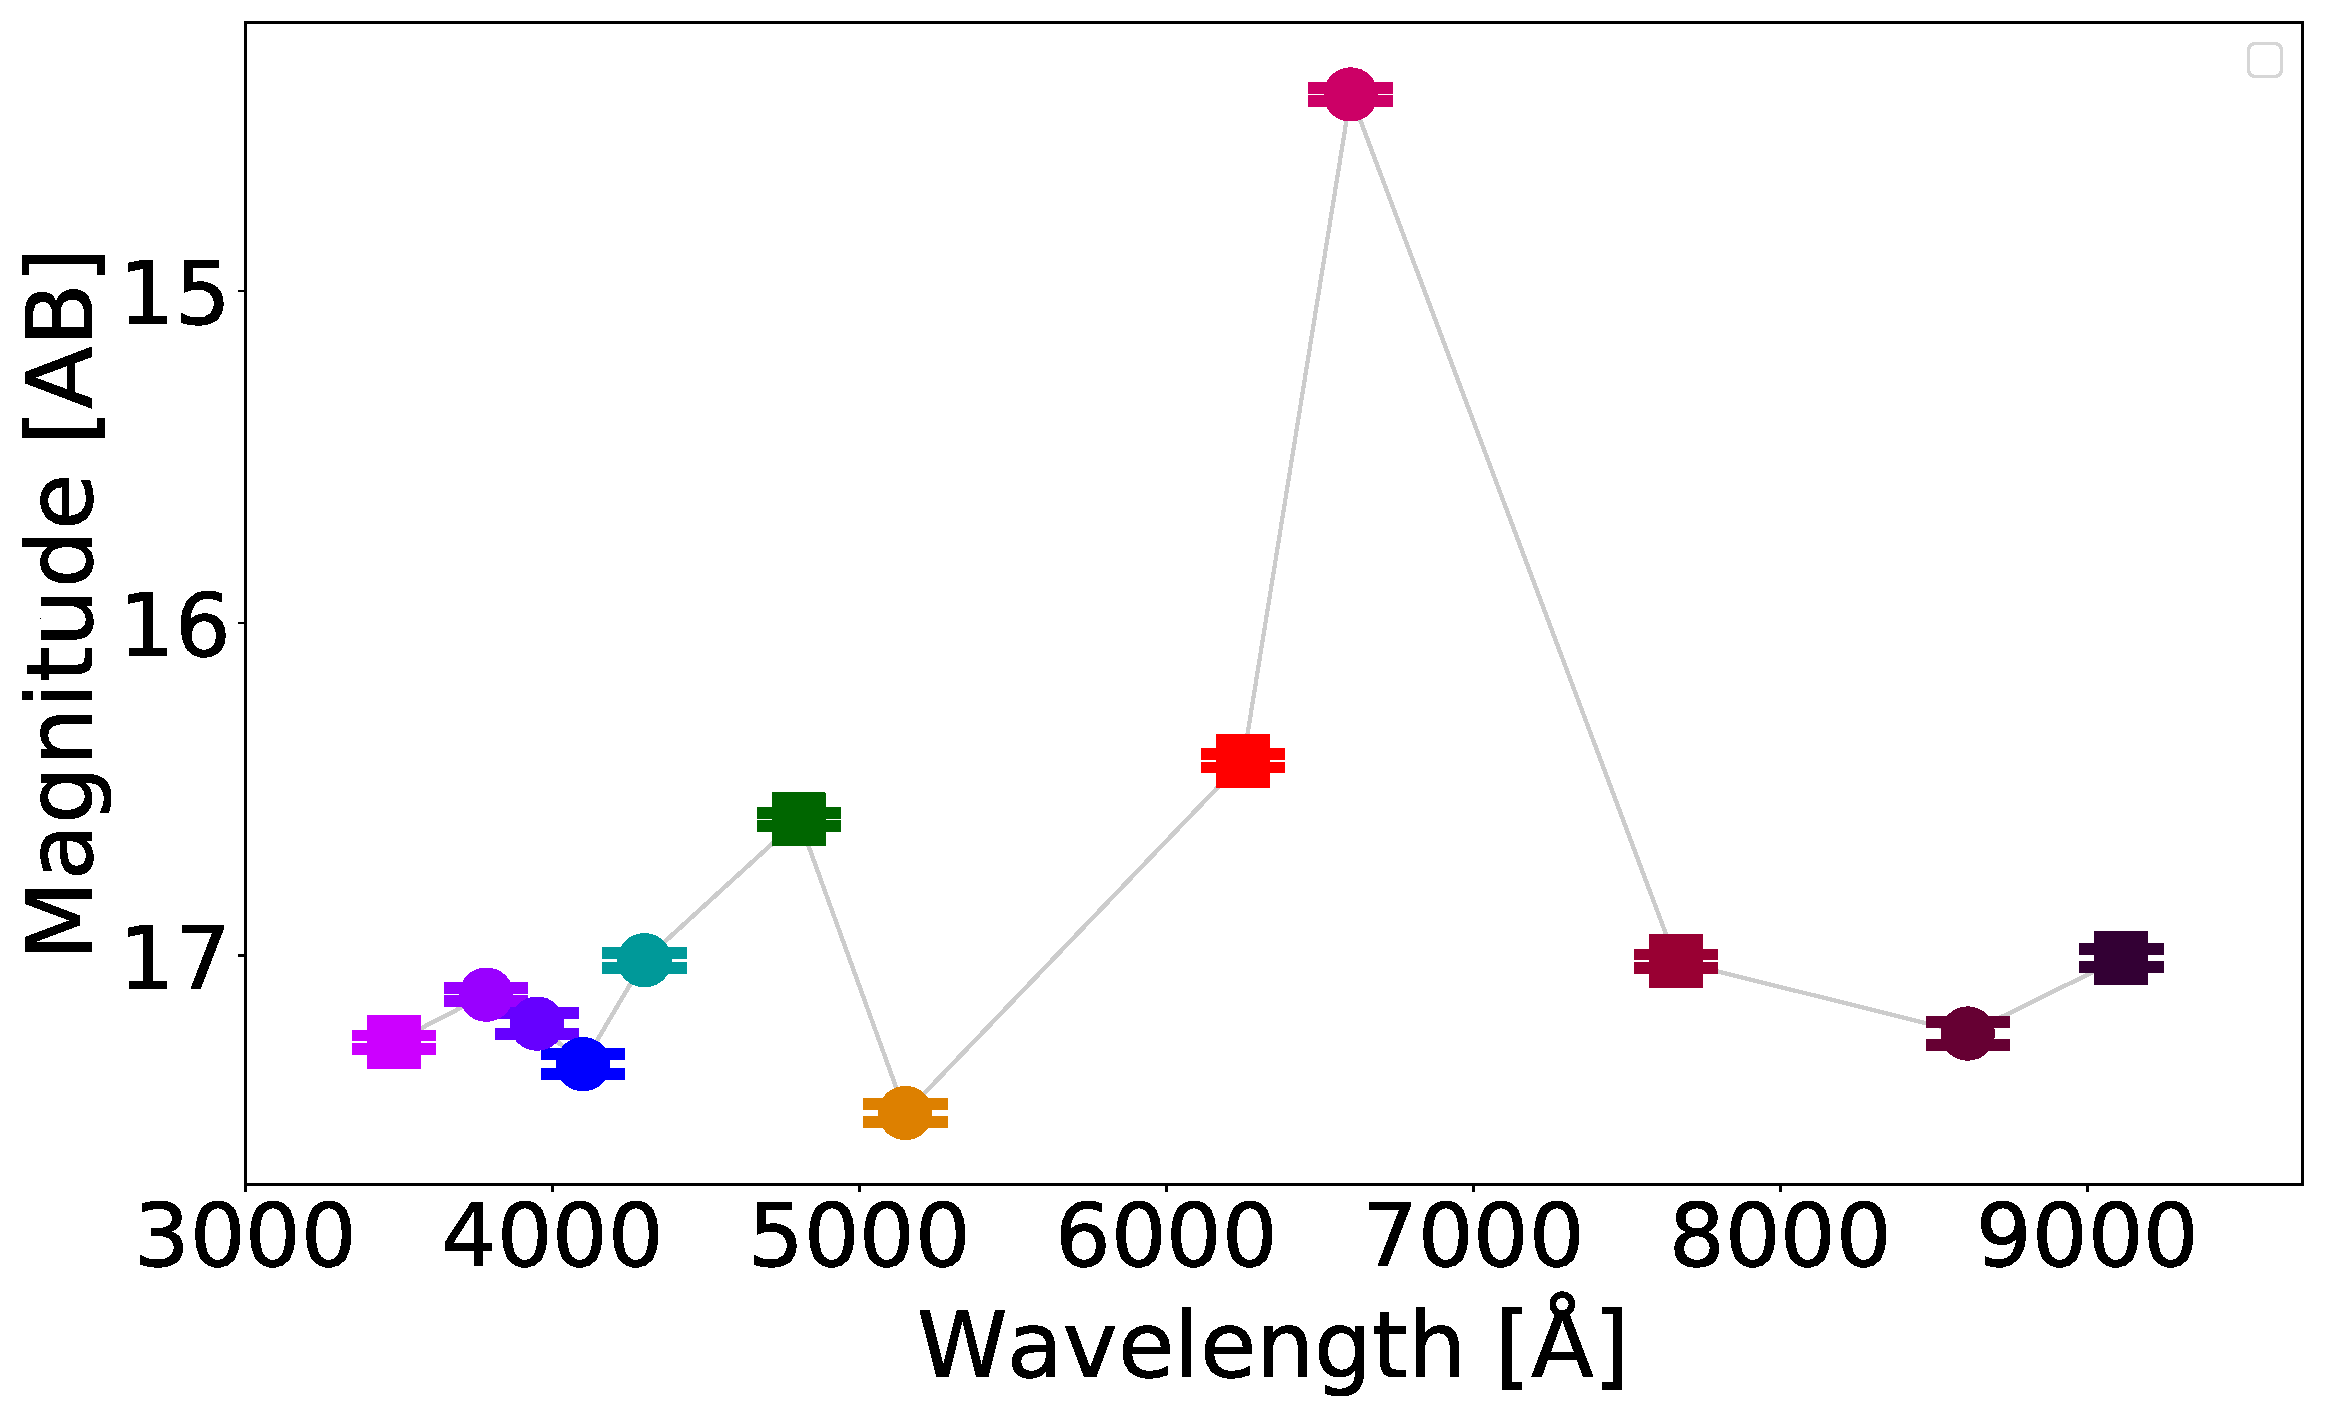
\includegraphics[width=0.3\linewidth, clip]{photopectrum_splus_MC0113-084466_auto.pdf} & 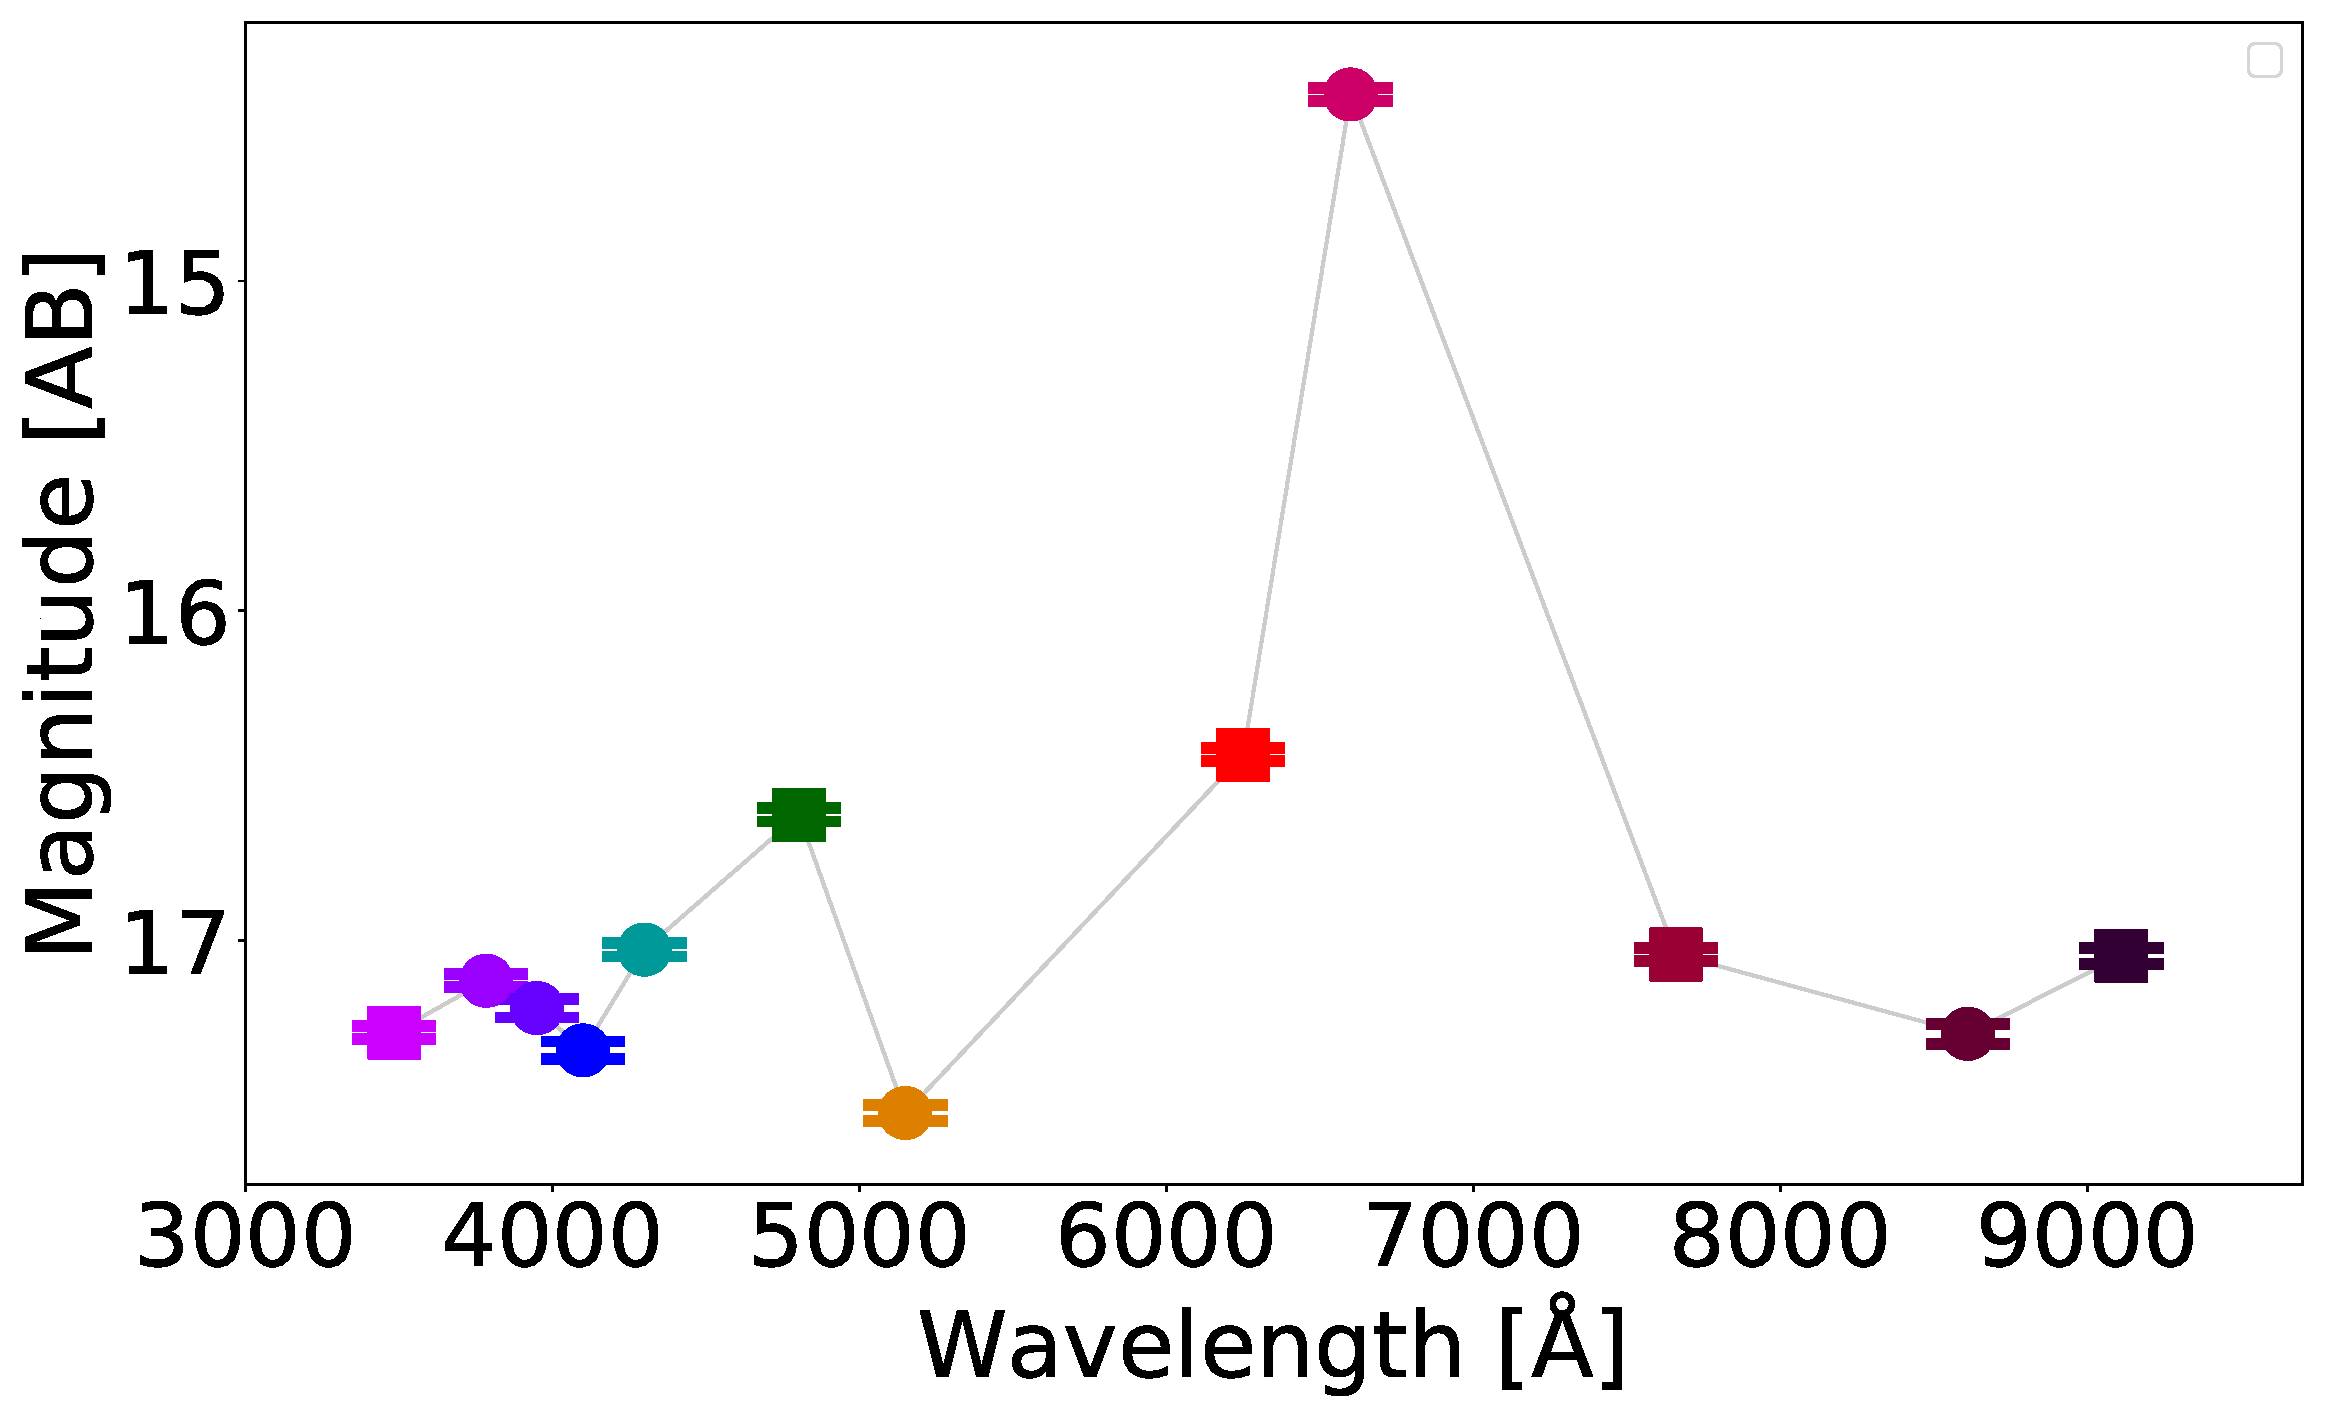
\includegraphics[width=0.3\linewidth, clip]{photopectrum_splus_MC0113-084466_petro.pdf} \\
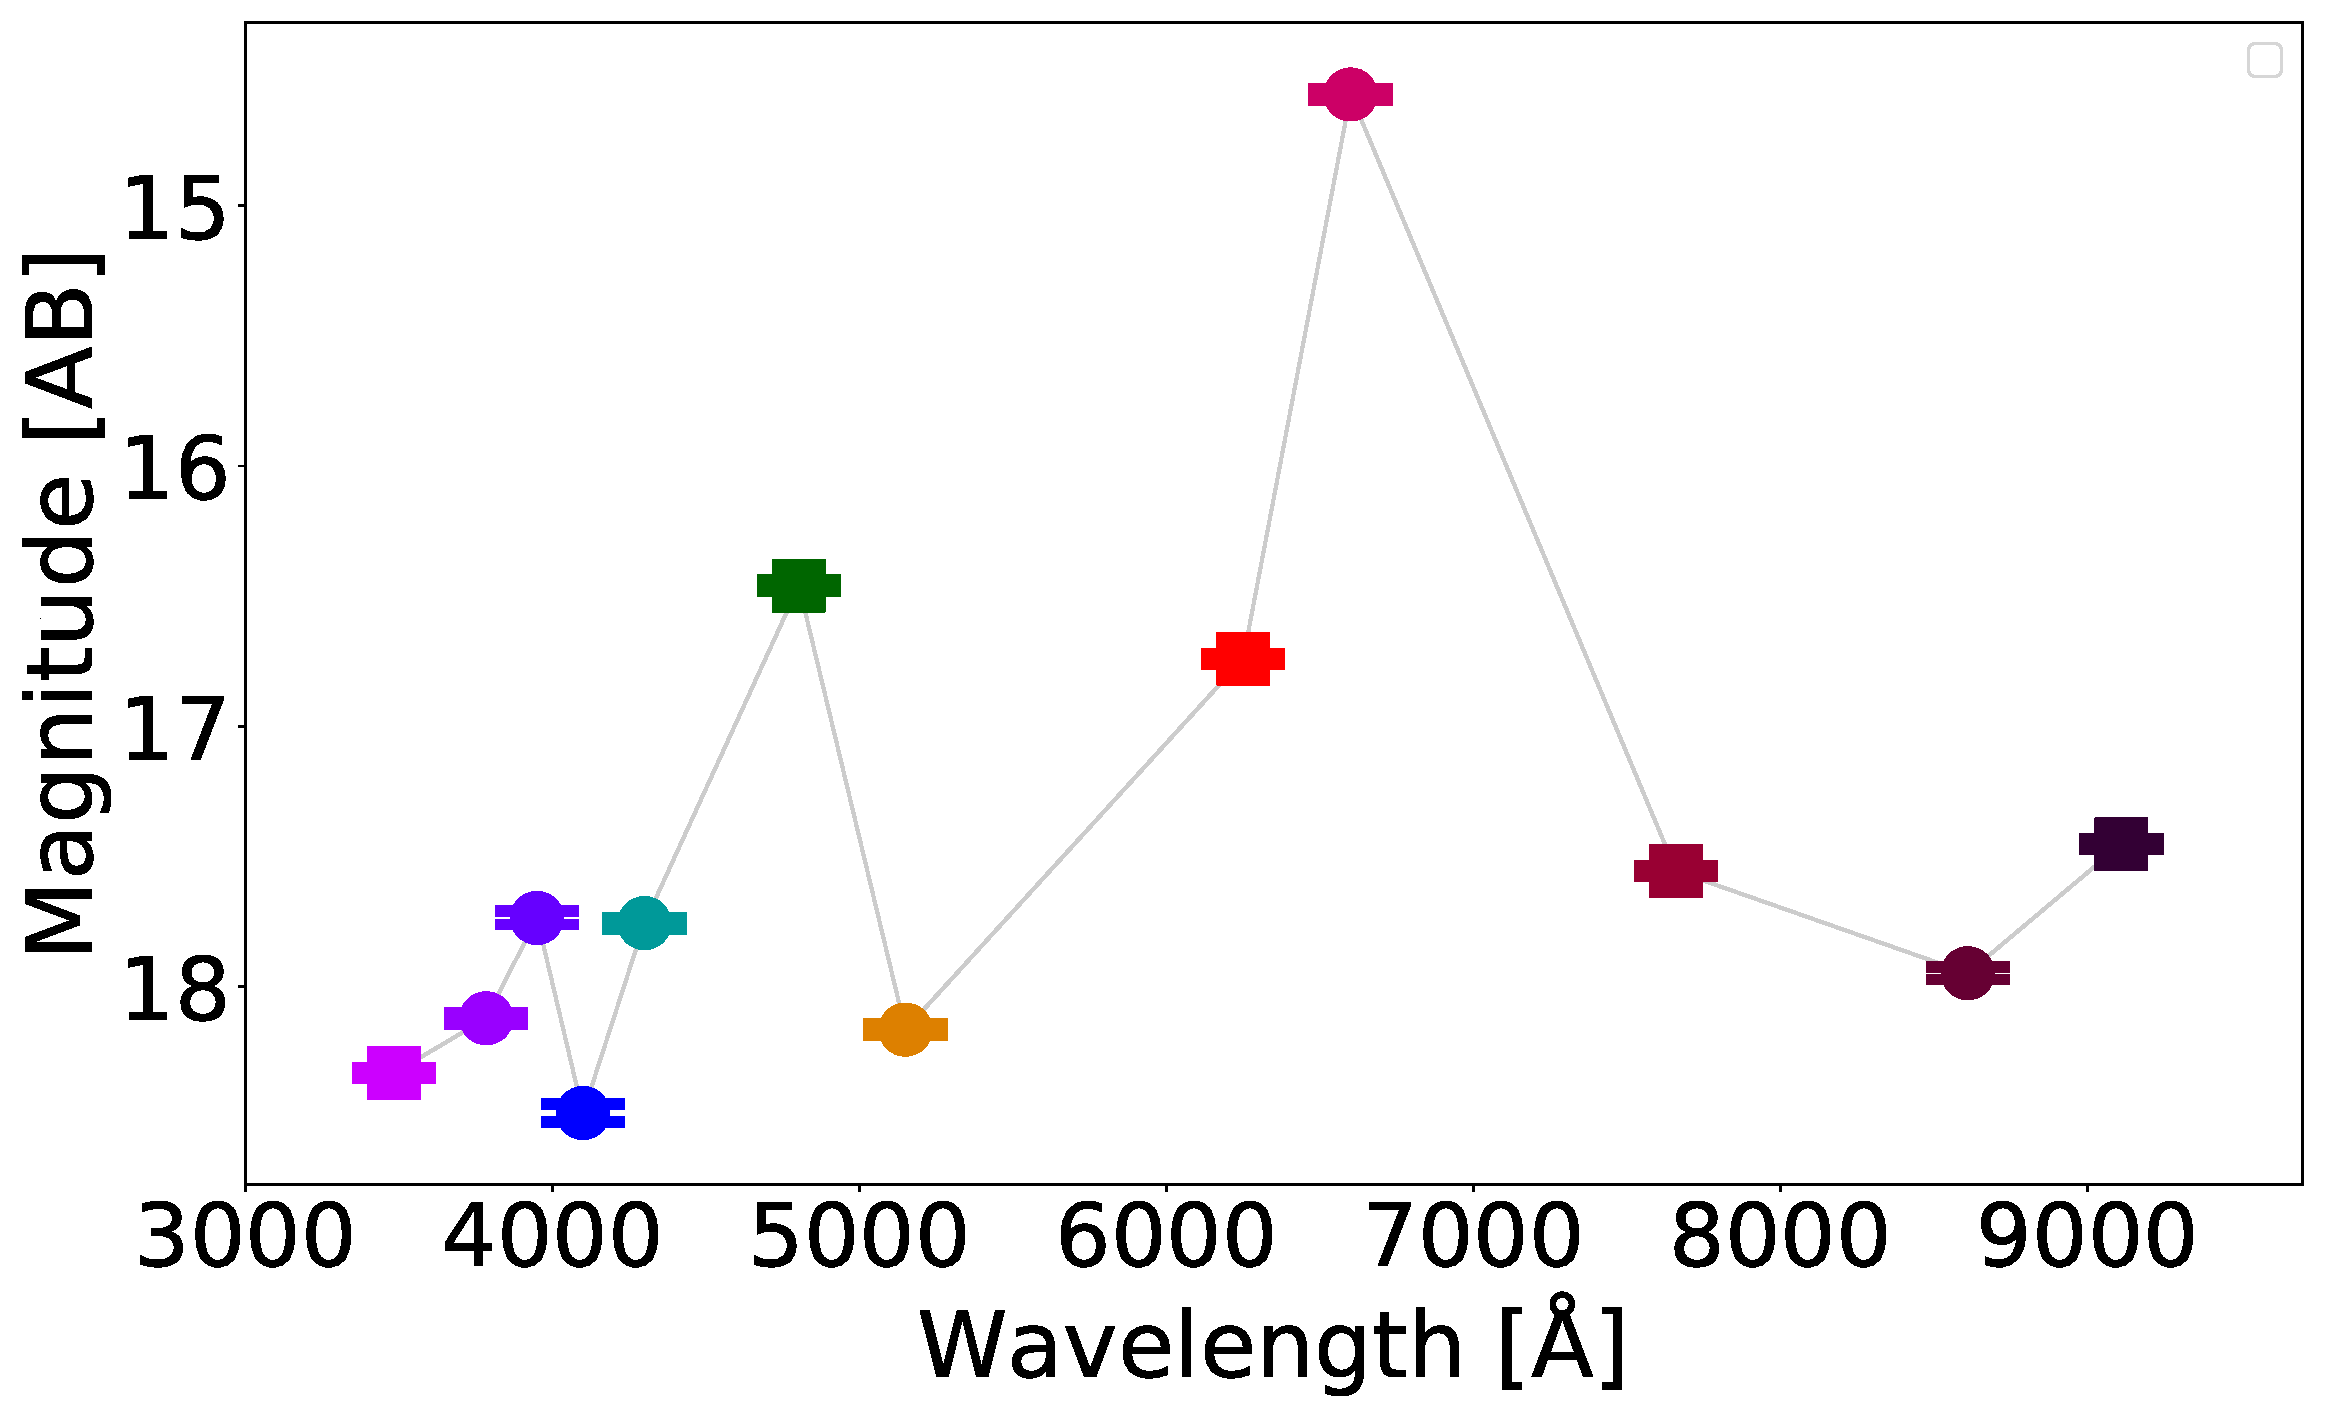
\includegraphics[width=0.3\linewidth, clip]{photopectrum_splus_MC0114-113862_aper.pdf} & 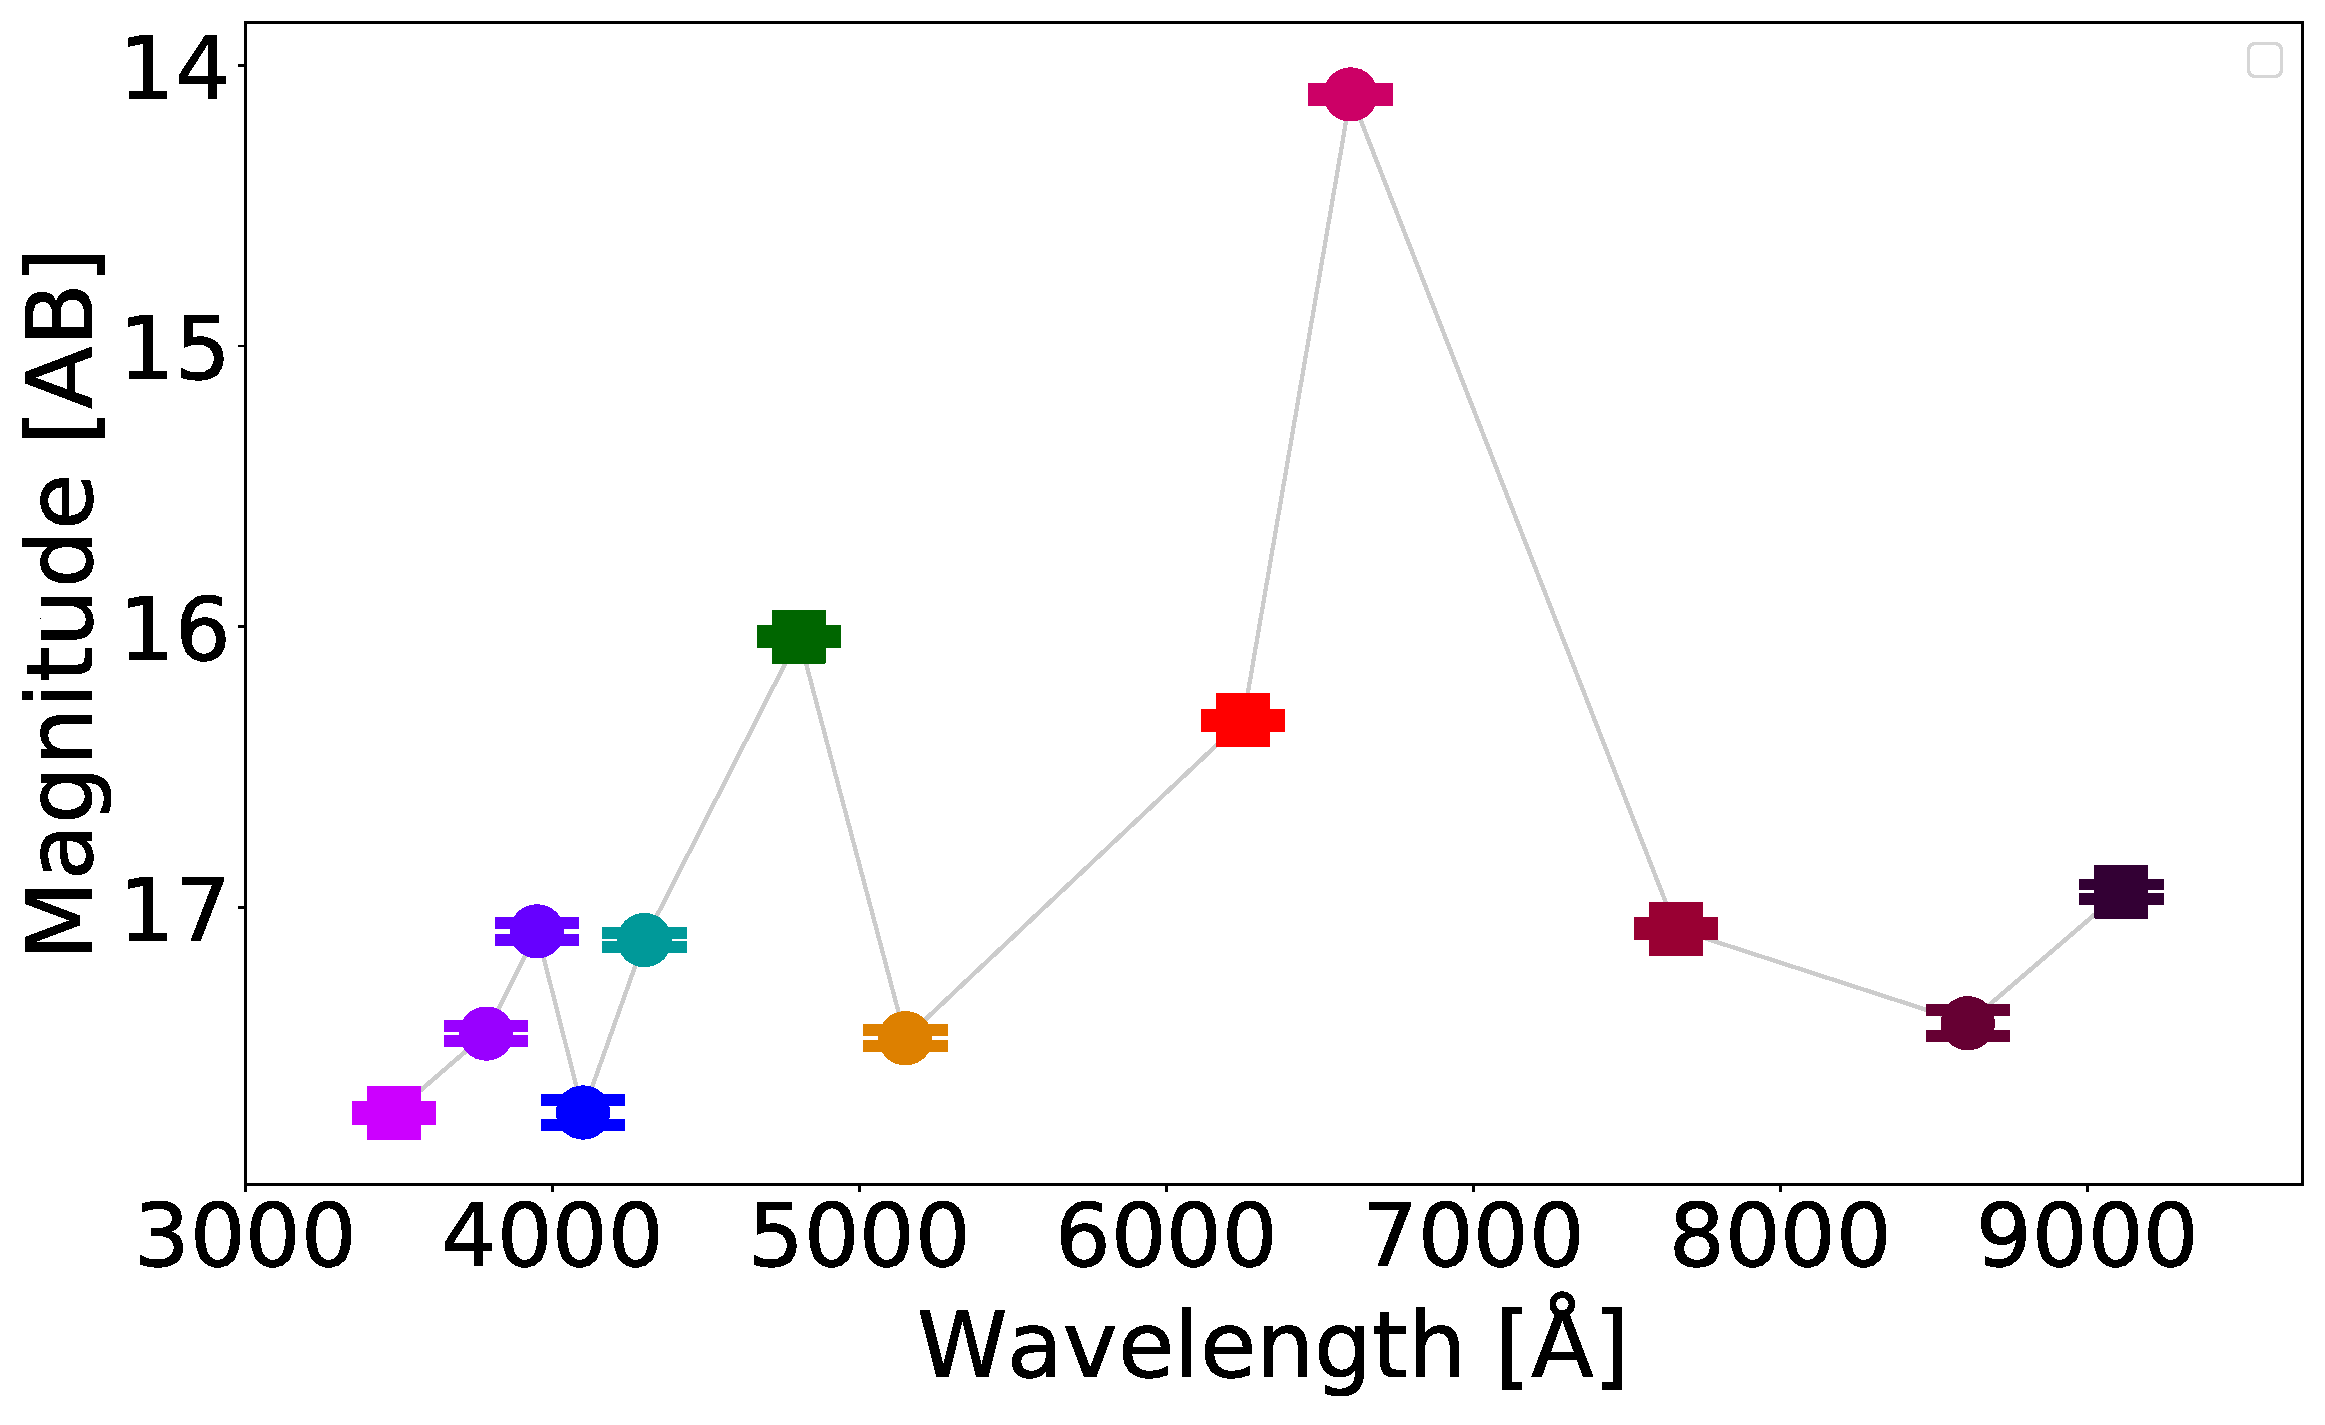
\includegraphics[width=0.3\linewidth, clip]{photopectrum_splus_MC0114-113862_auto.pdf} & 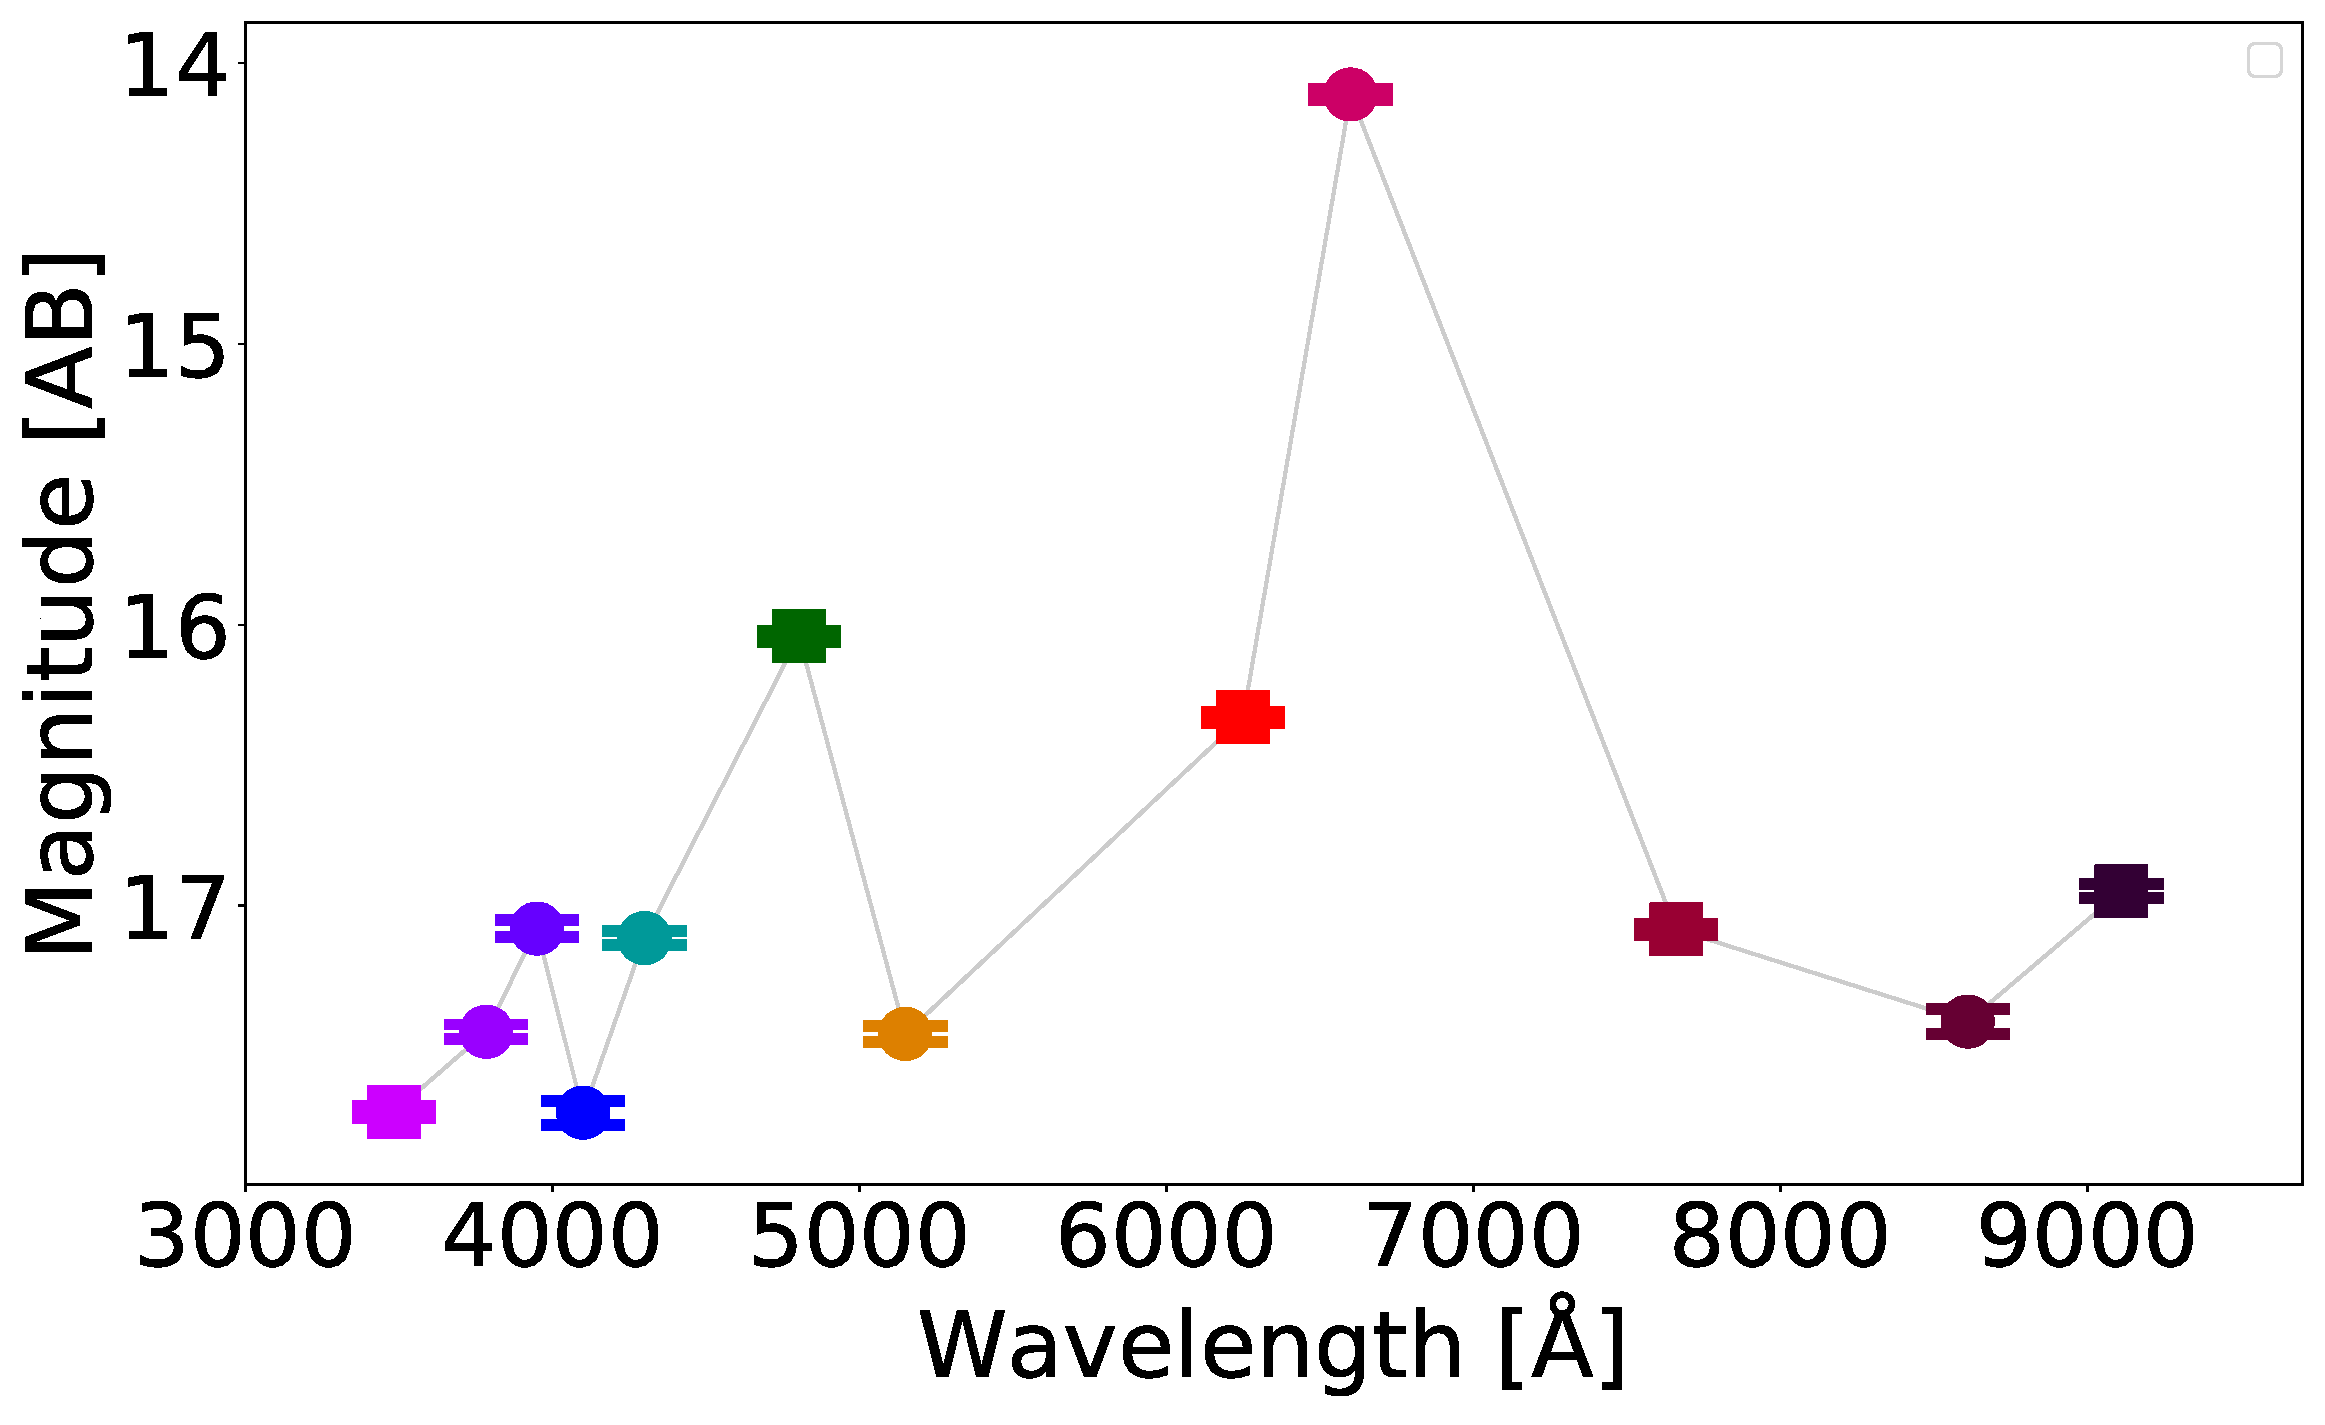
\includegraphics[width=0.3\linewidth, clip]{photopectrum_splus_MC0114-113862_petro.pdf} \\

\end{tabular}
\end{table}

\end{longtable}
% \newpage
% \begin{center}[!h]
% \begin{longtable}{ccc}
% %\caption{A sample long table.} \label{tab:long} \\

%  \multicolumn{1}{c}{\textbf{Aper (3'')}} & \multicolumn{1}{c}{\textbf{F515+F660+F861}} & \multicolumn{1}{c}{\textbf{G+R+I}} \\ 
% \endfirsthead

% % \multicolumn{3}{c}%
% % {{\bfseries \tablename\ \thetable{} -- continued from previous page}} \\
% %  \multicolumn{1}{c}{\textbf{Aper (3'')}} & \multicolumn{1}{c}{\textbf{F515+F660+F861}} & \multicolumn{1}{c}{\textbf{G+R+I}} \\ 
% % \endhead

% \multicolumn{3}{r}{{Continued on next page}} \\
% \endfoot

% \endlastfoot

% %\begin{table}
%\begin{tabular}{ccc}
\textbf{Aper(3'')} & \textbf{F515+F660+F861} & \textbf{G+R+I} \\
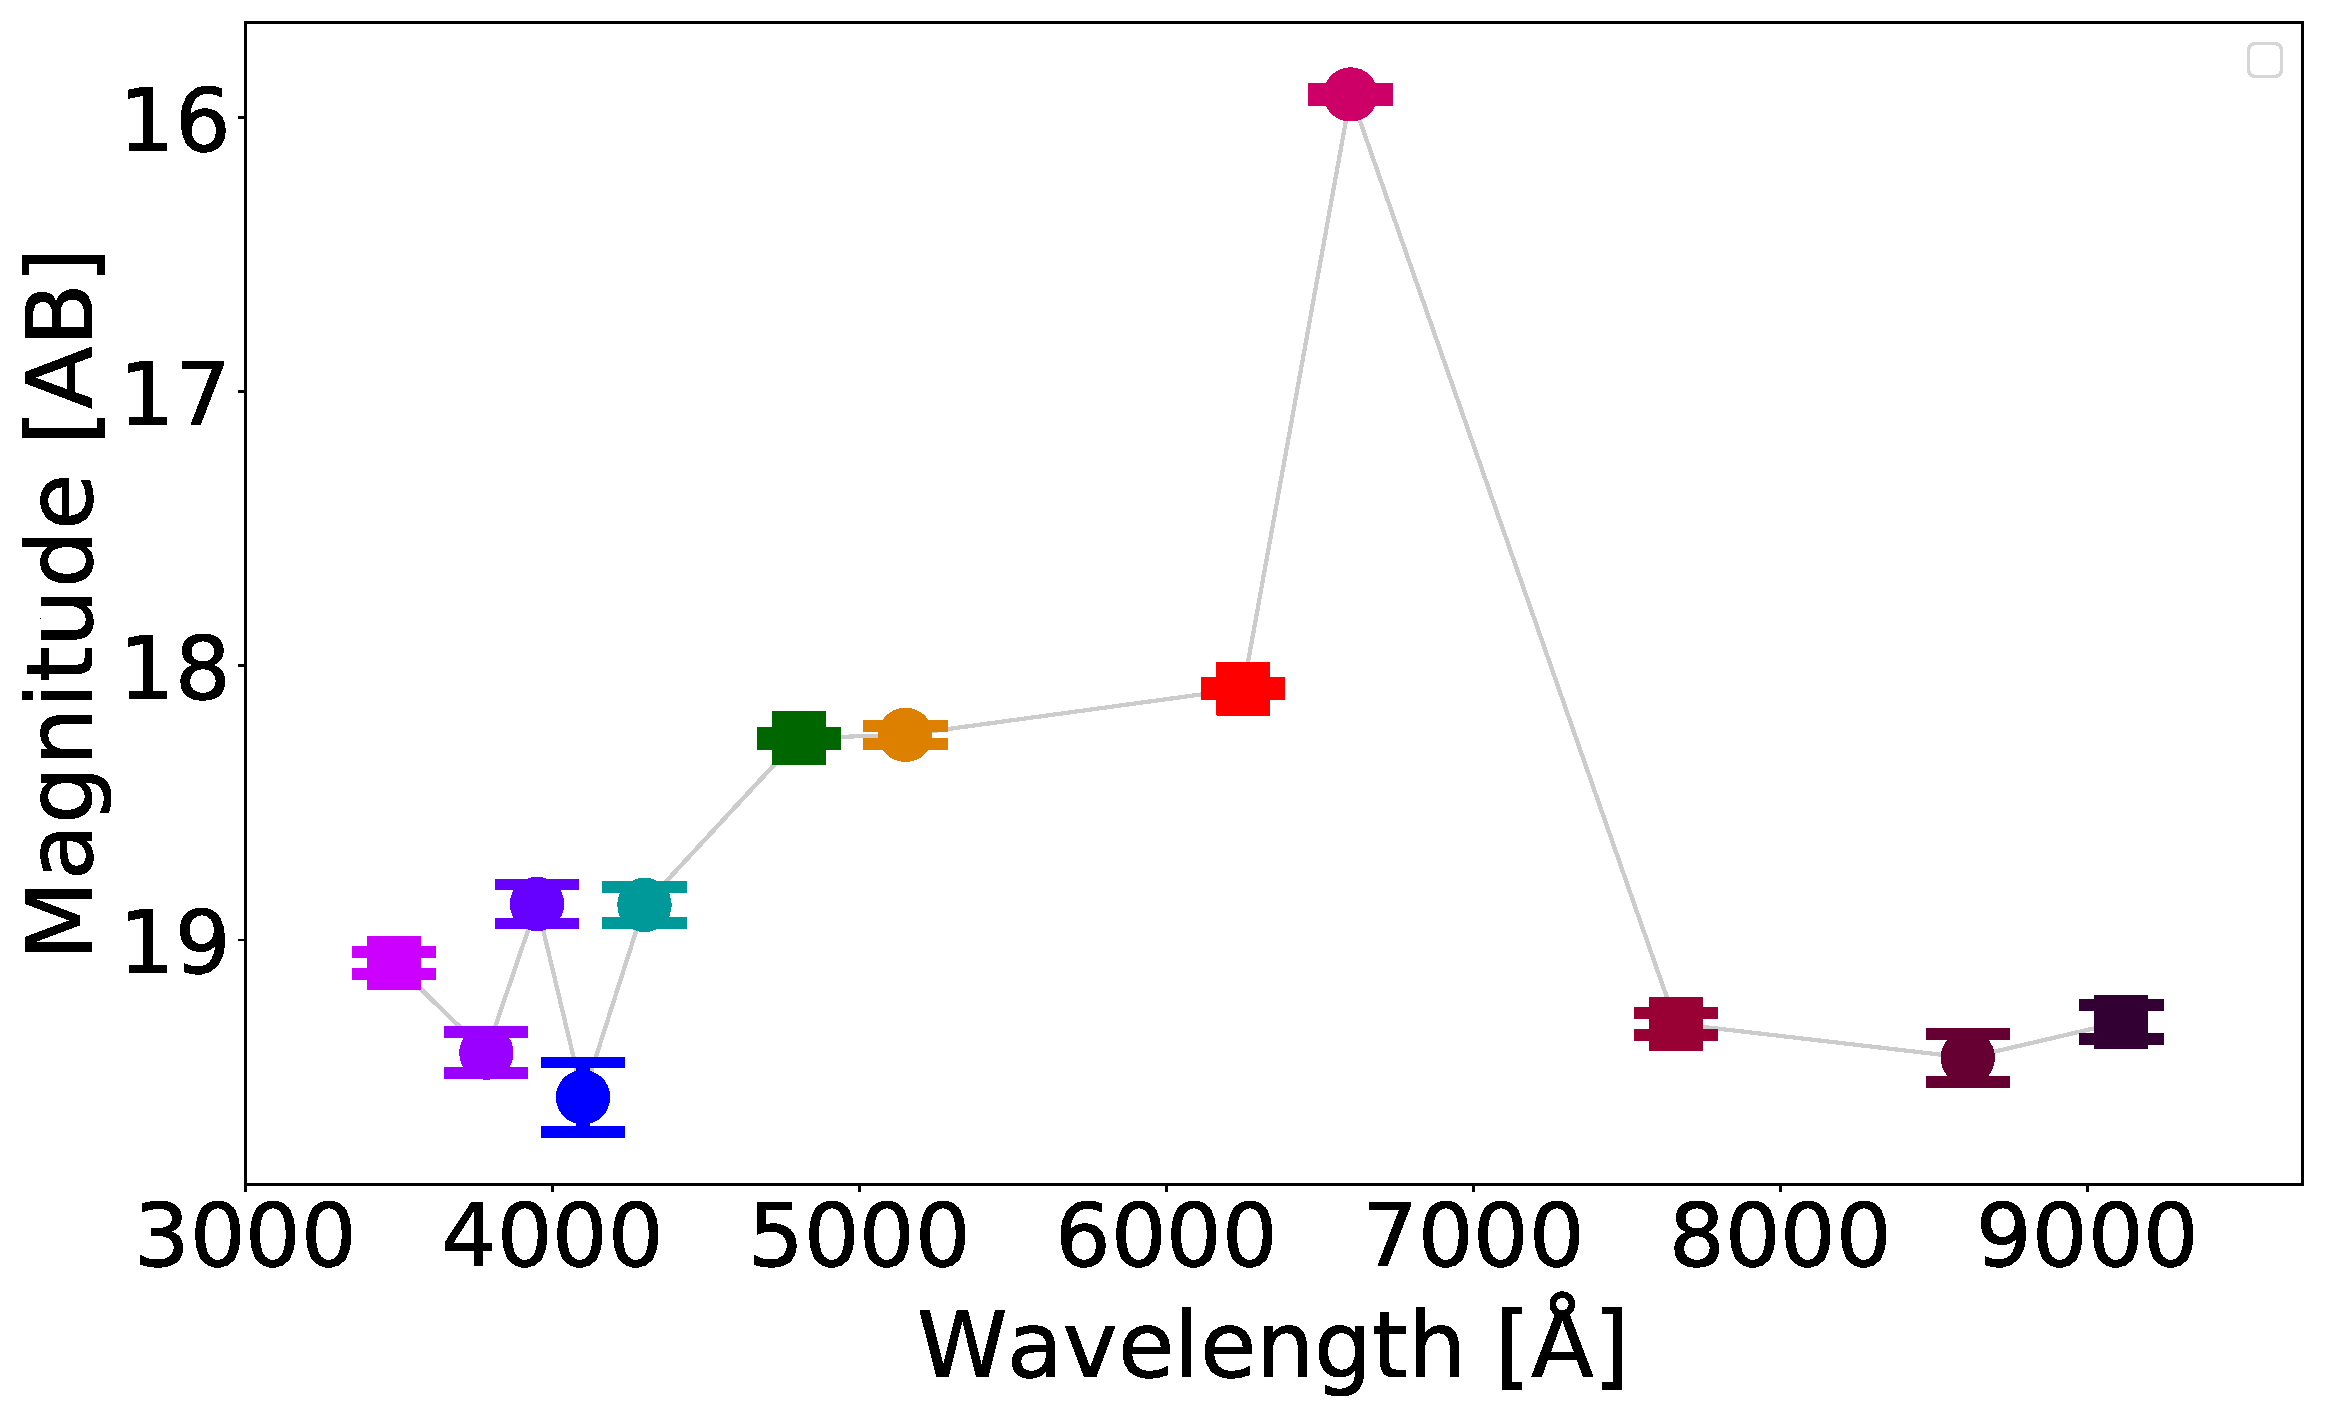
\includegraphics[width=0.3\linewidth, clip]{photopectrum_splus_MC0072-006125_aper.pdf} & 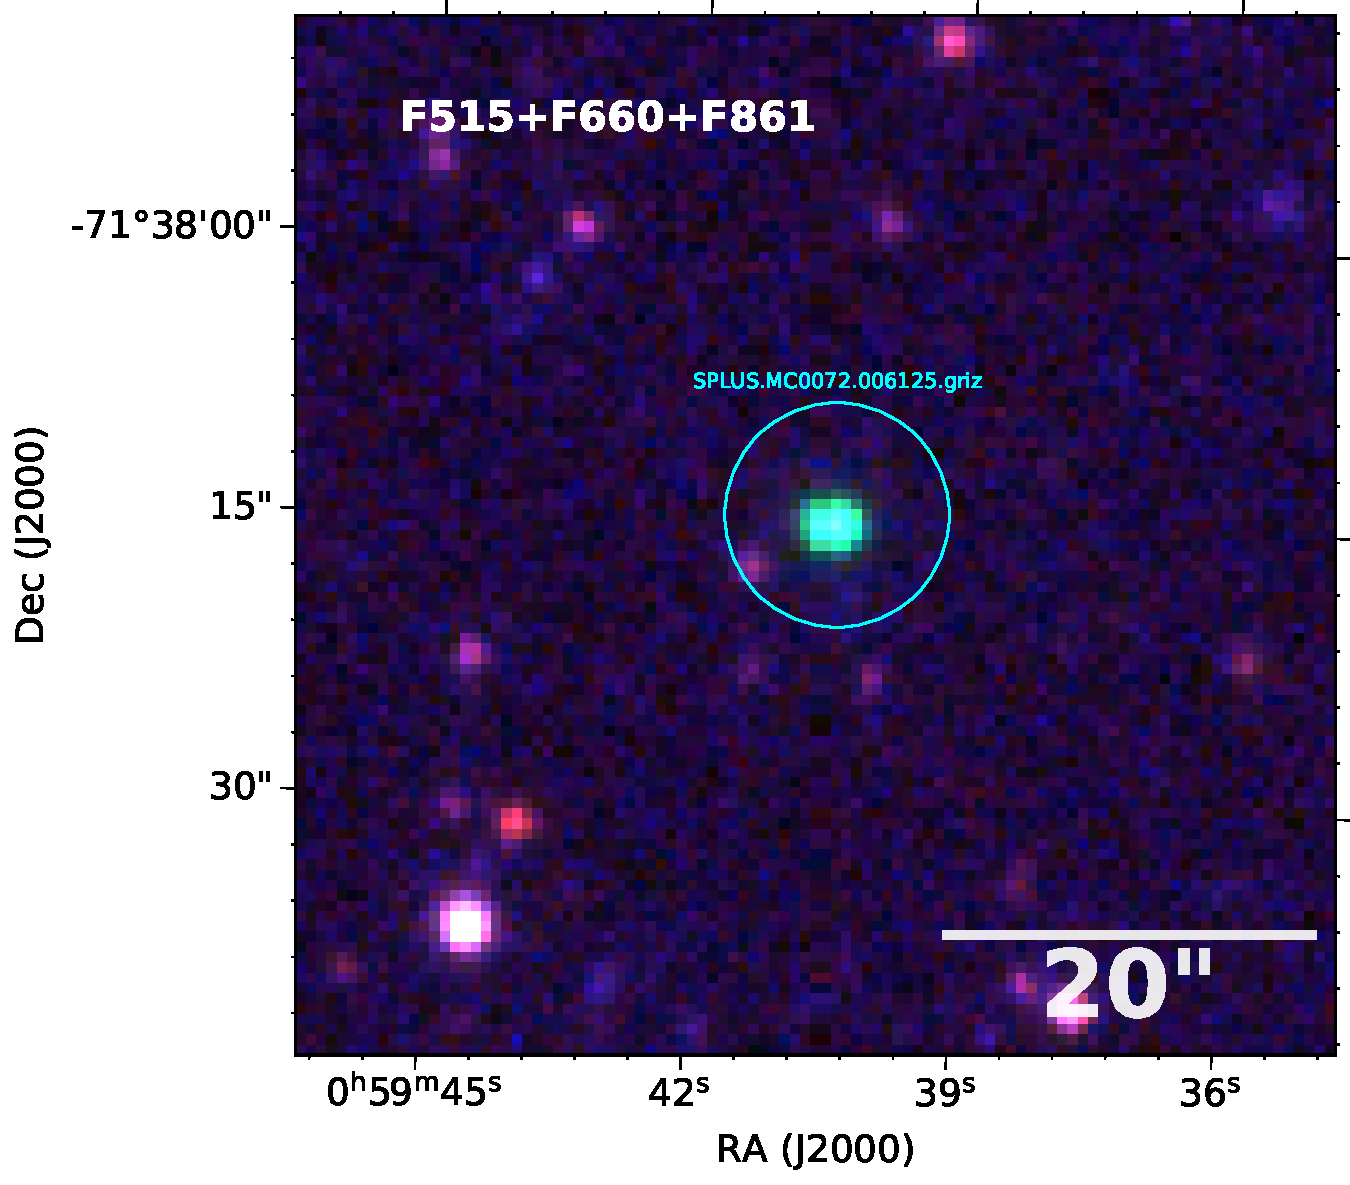
\includegraphics[width=0.3\linewidth, clip]{MC0072/MC0072_F861_006125-RGB.pdf} & 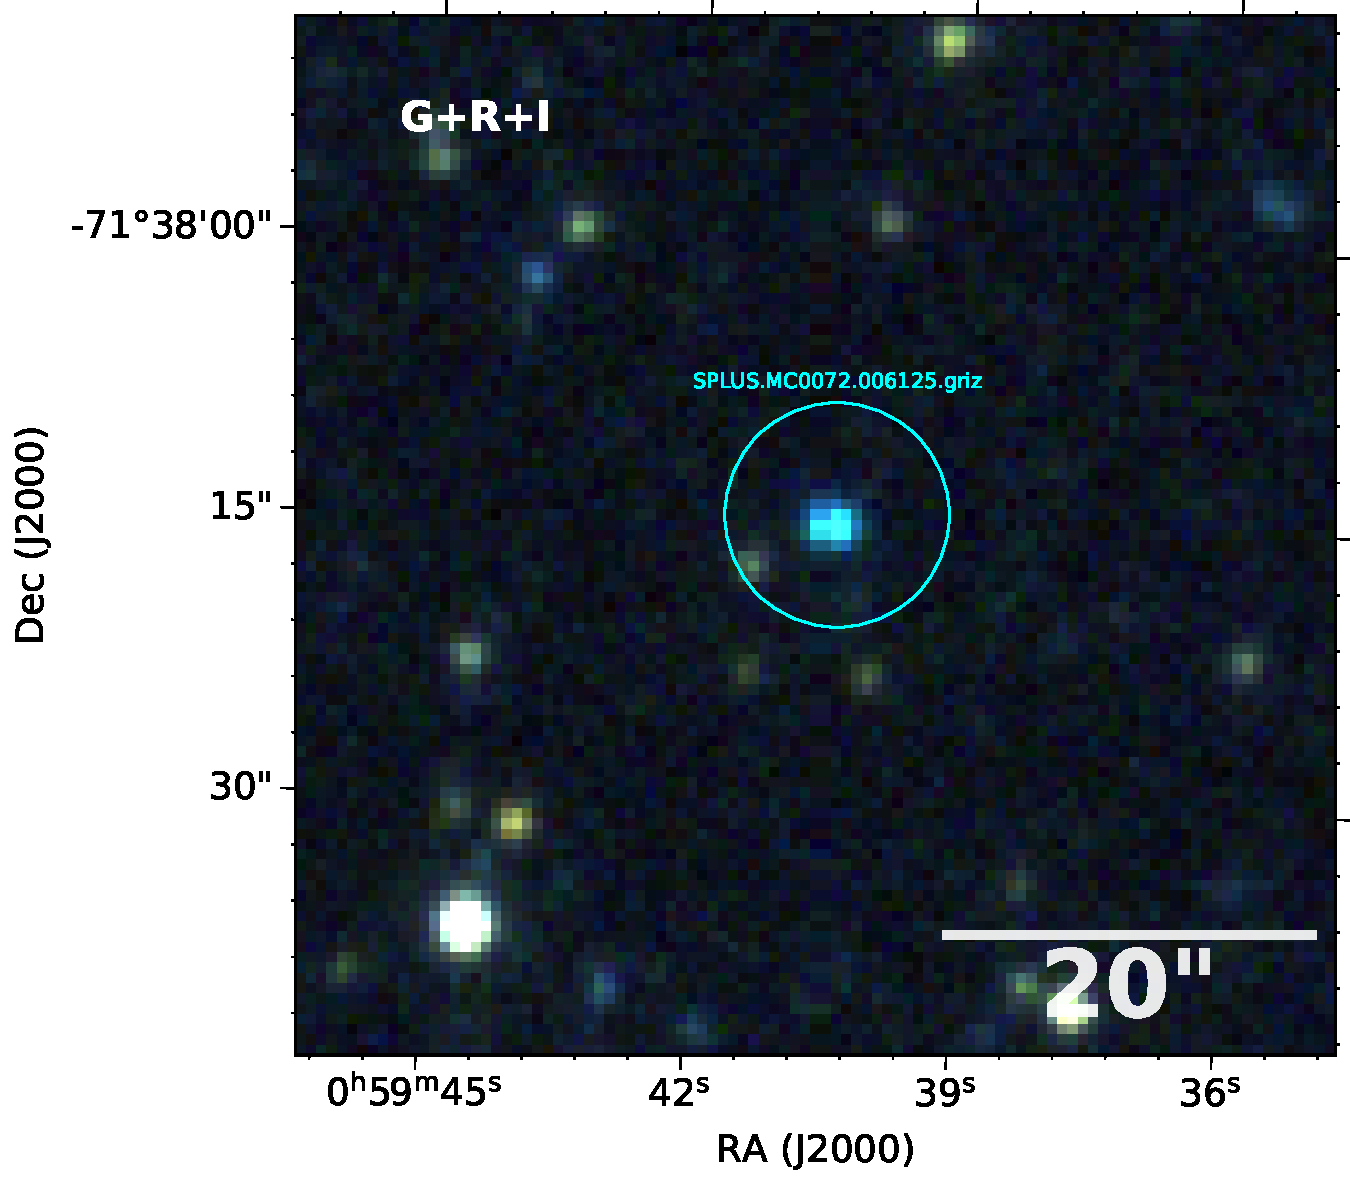
\includegraphics[width=0.3\linewidth, clip]{MC0072/MC0072_I_006125-RGB.pdf} \\
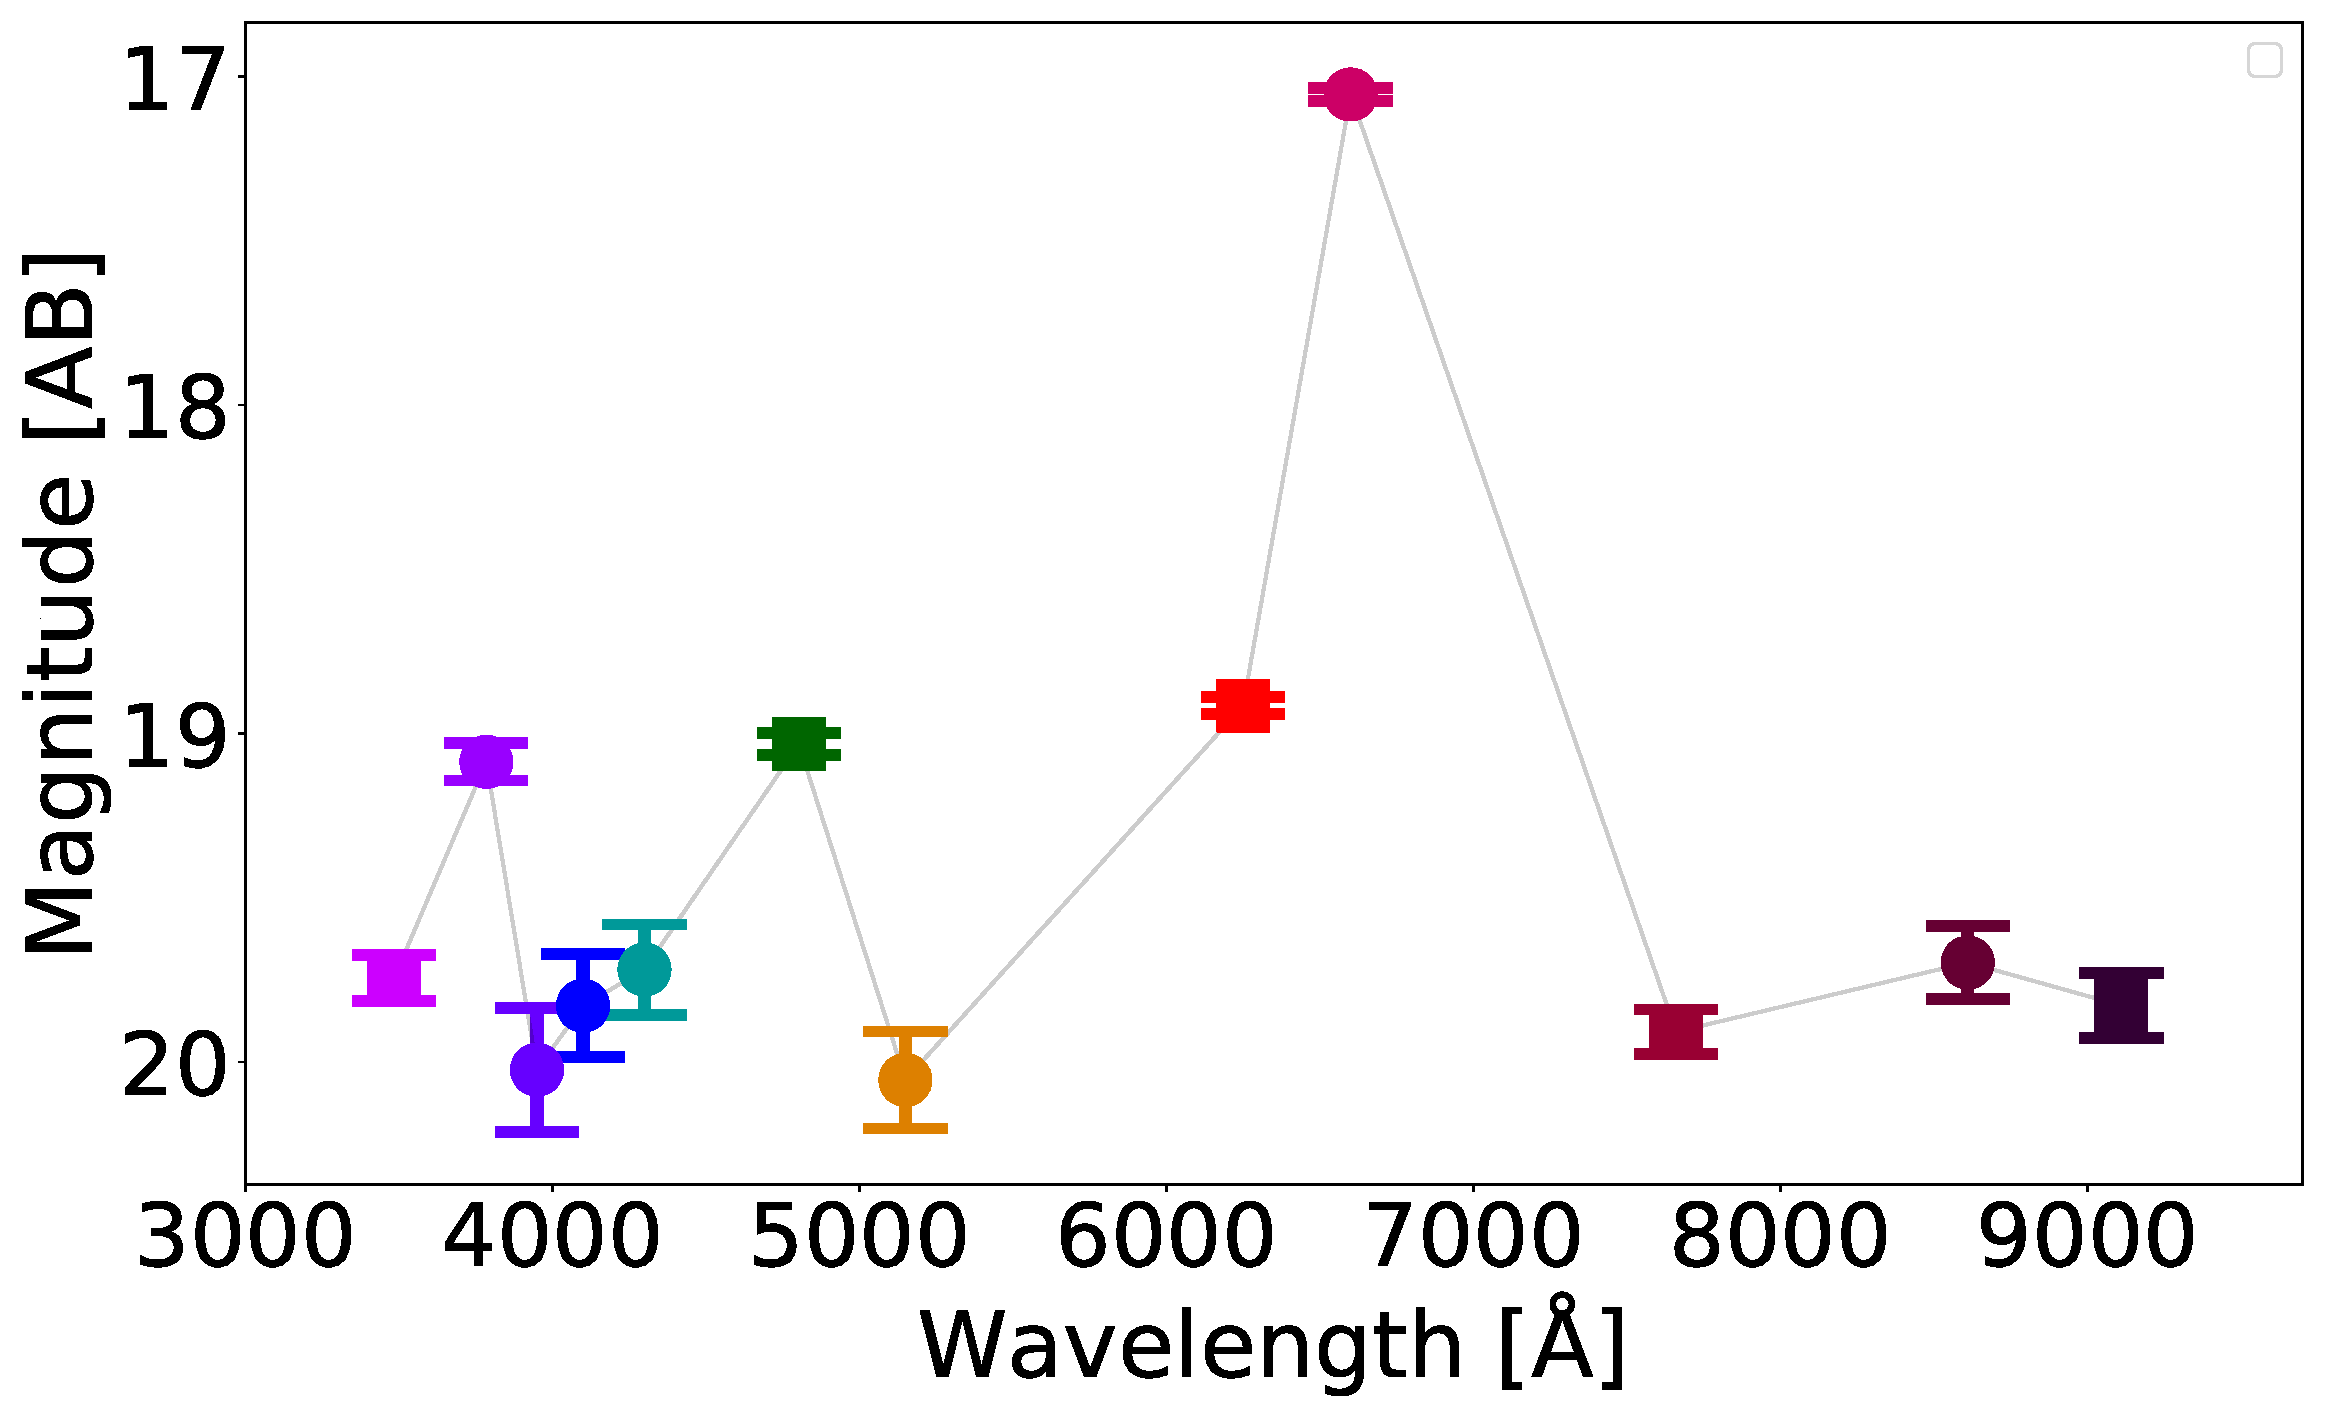
\includegraphics[width=0.3\linewidth, clip]{photopectrum_splus_MC0072-044863_aper.pdf} & 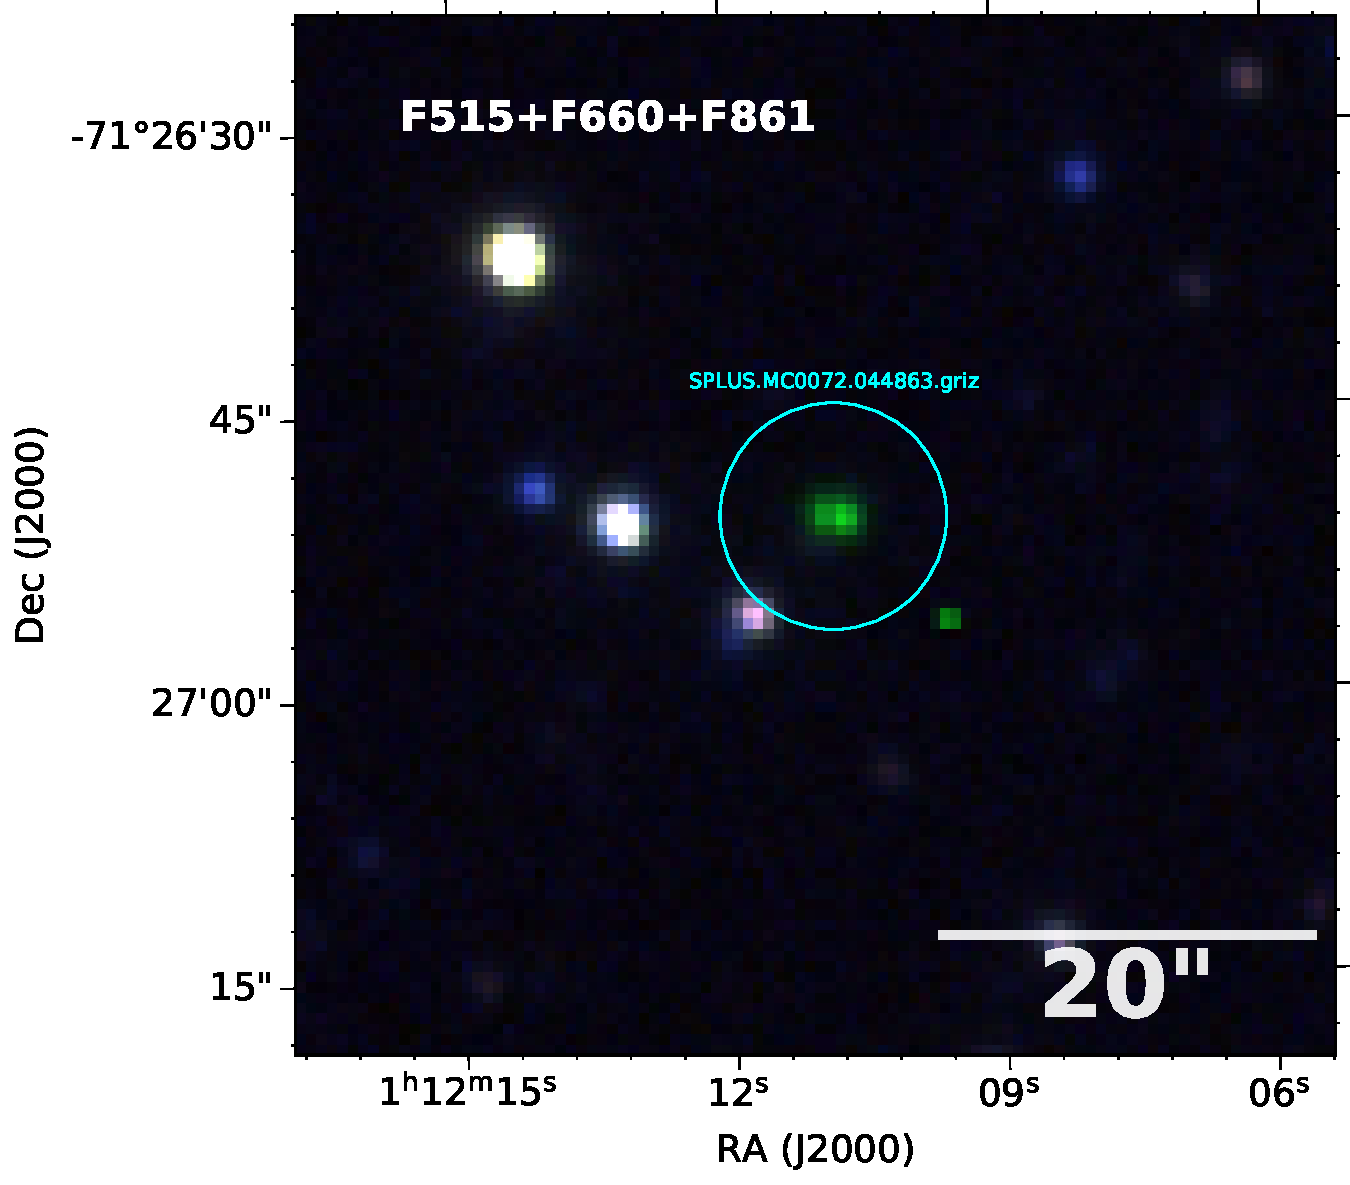
\includegraphics[width=0.3\linewidth, clip]{MC0072/MC0072_F861_044863-RGB.pdf} & 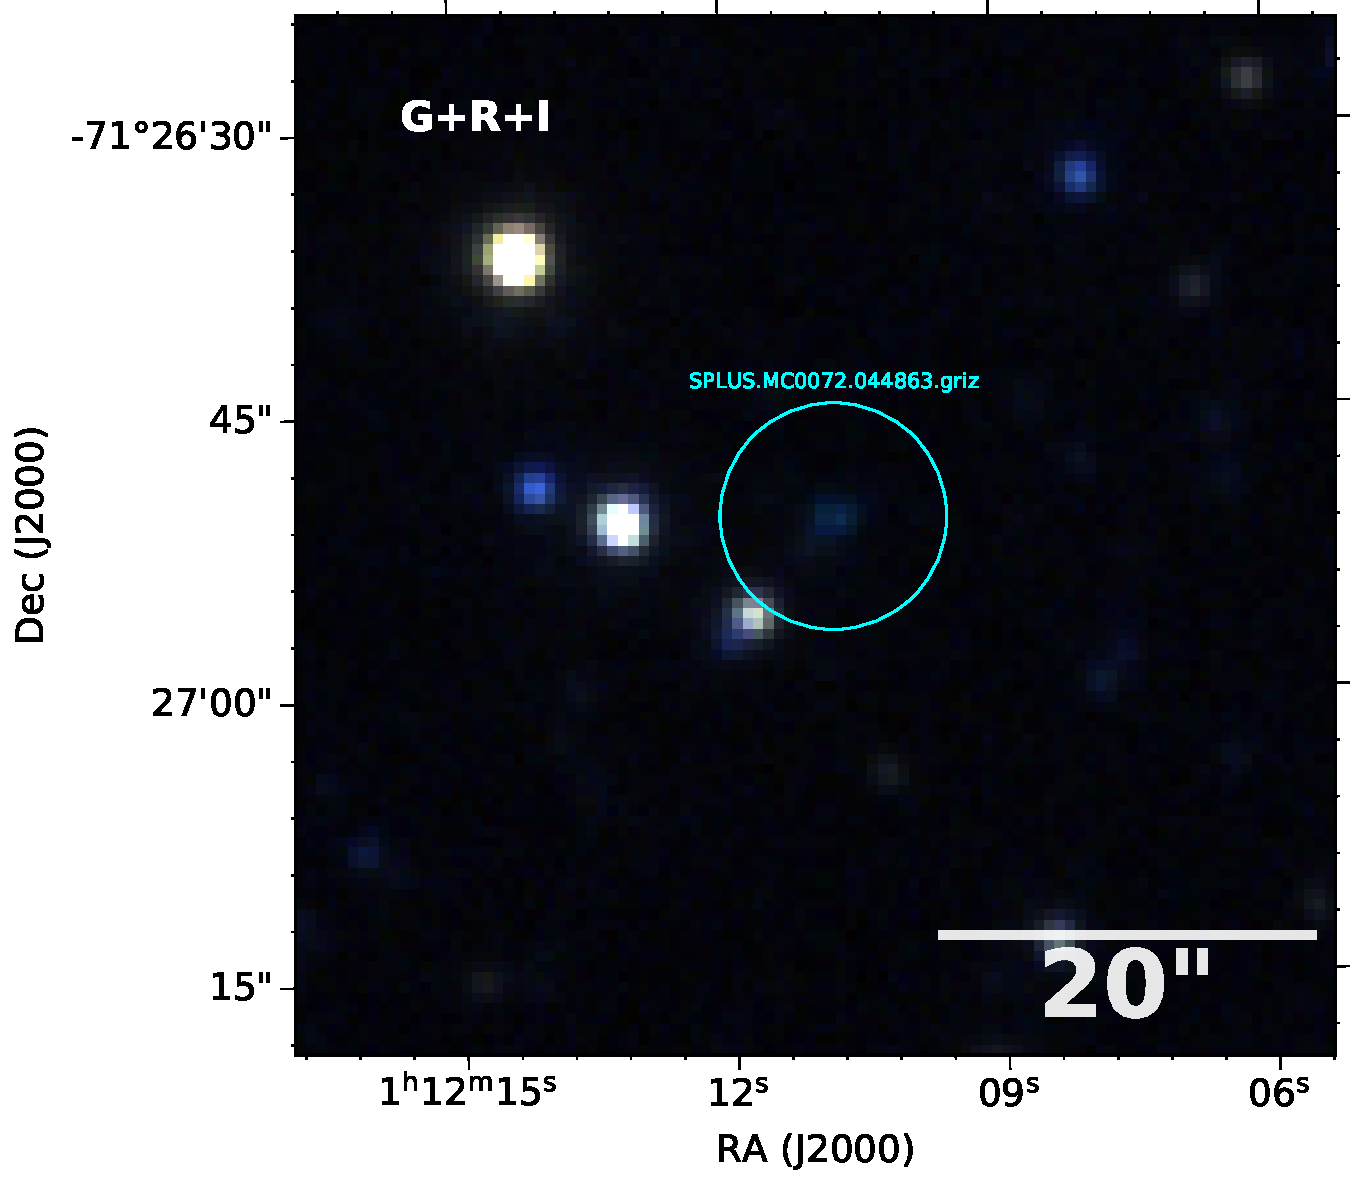
\includegraphics[width=0.3\linewidth, clip]{MC0072/MC0072_I_044863-RGB.pdf} \\
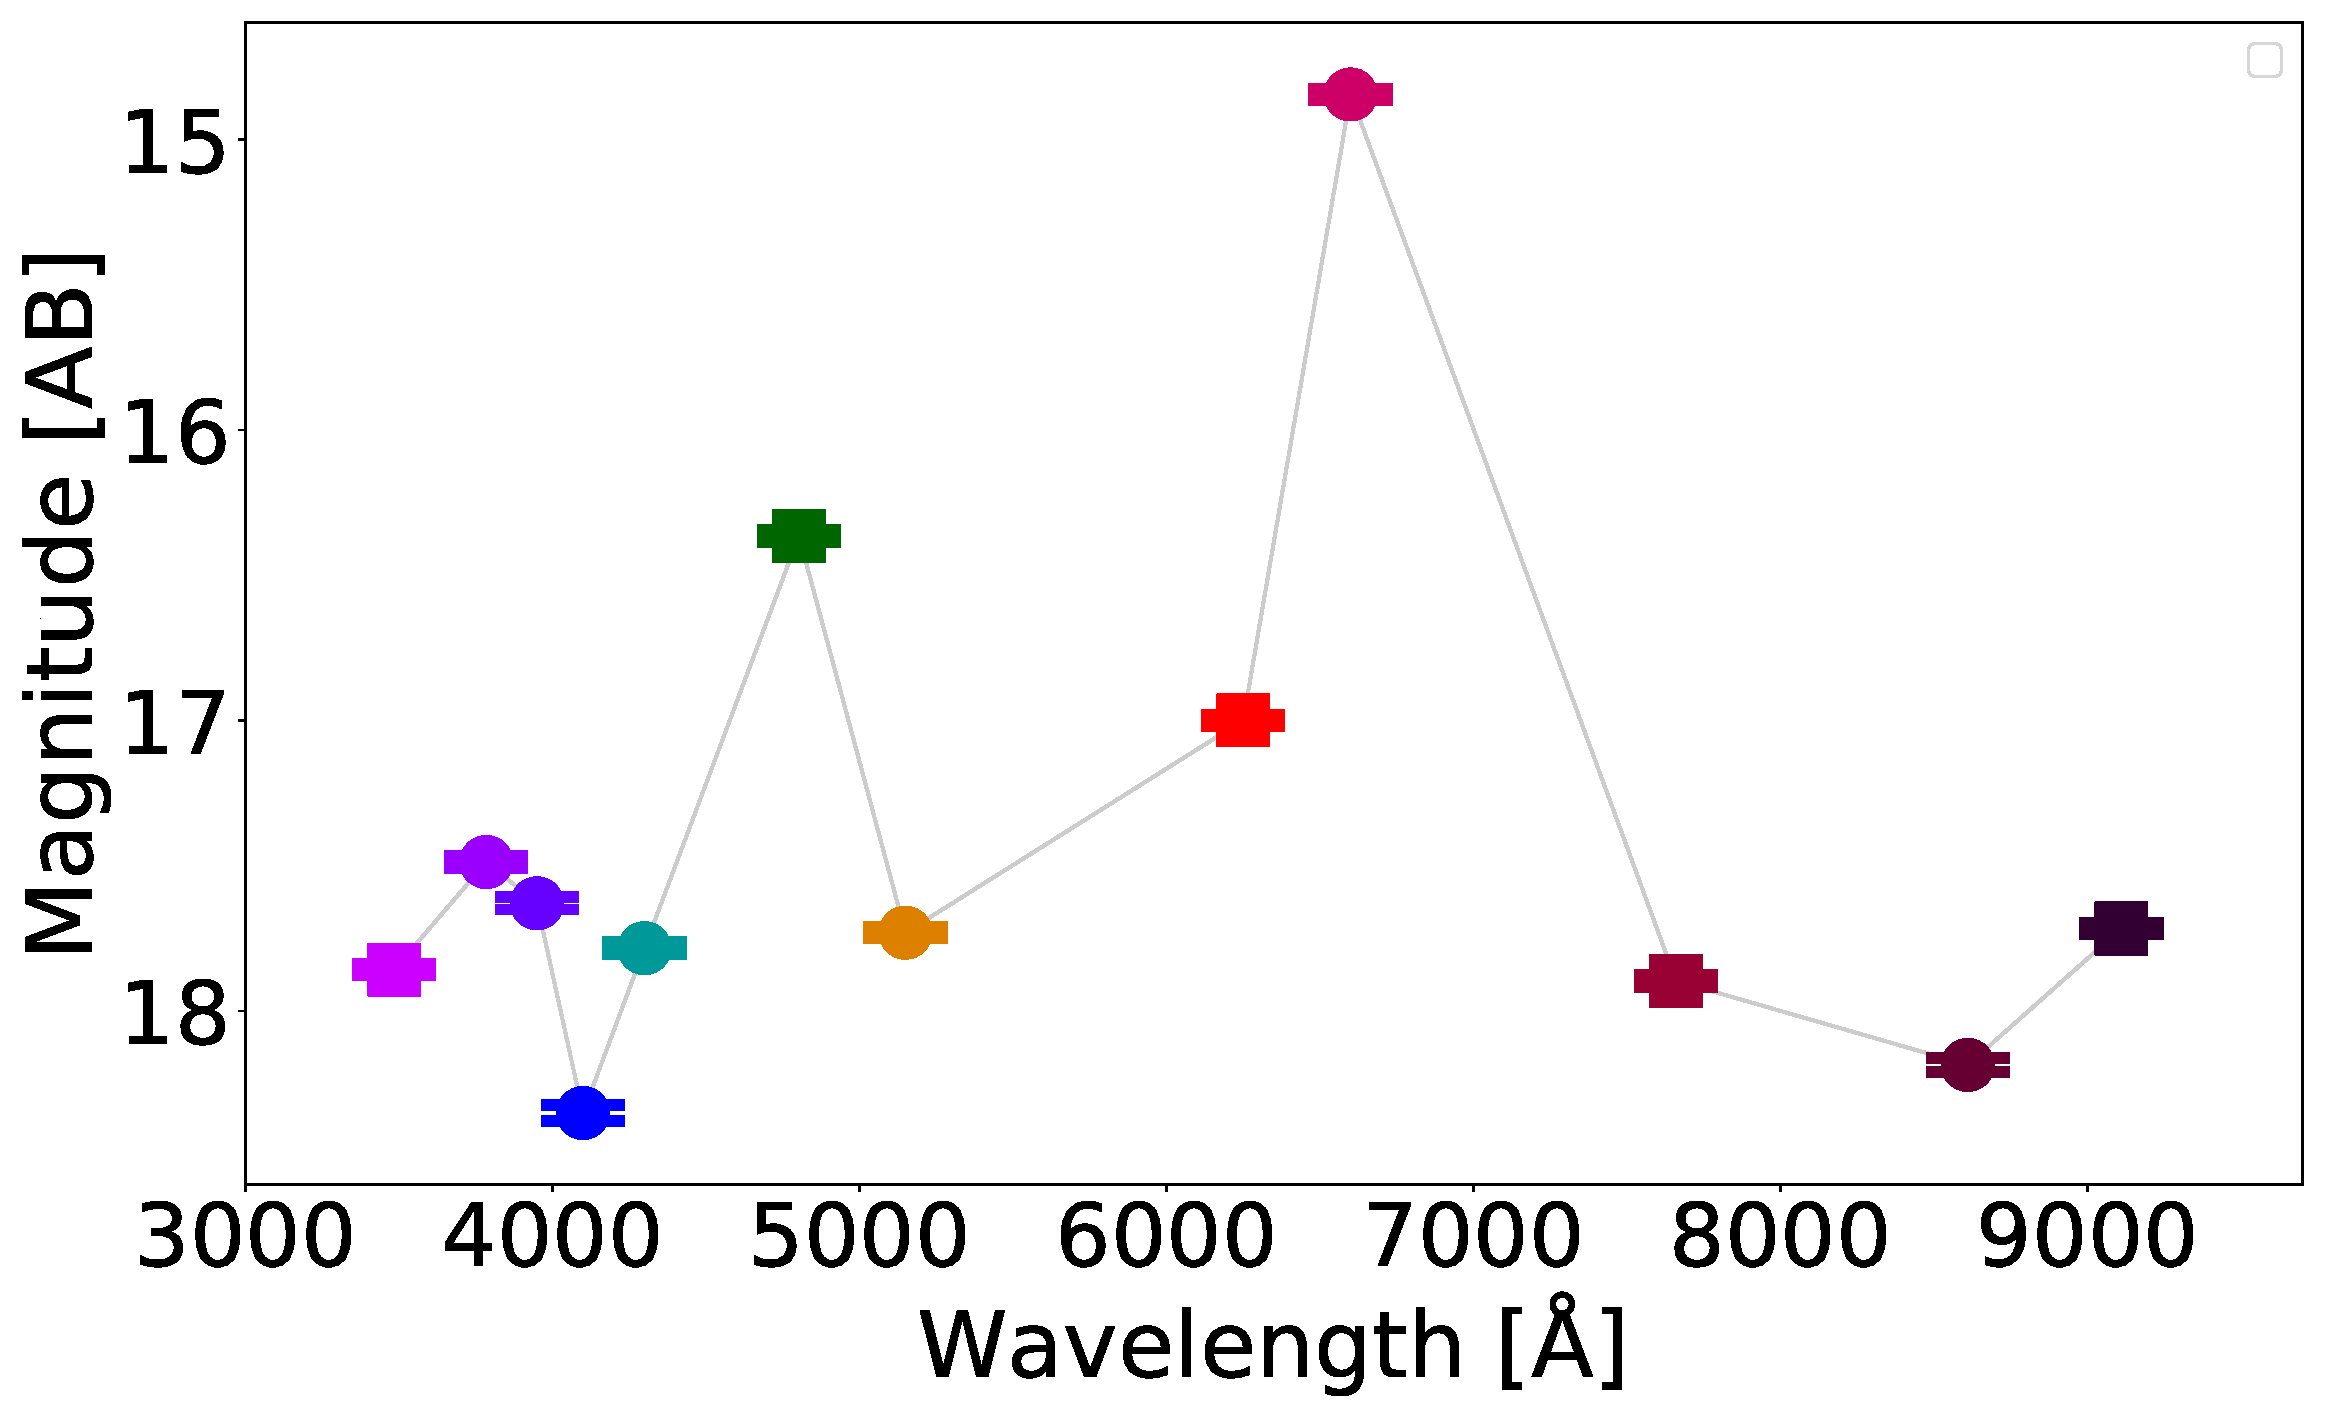
\includegraphics[width=0.3\linewidth, clip]{photopectrum_splus_MC0093-051819_aper.pdf} & 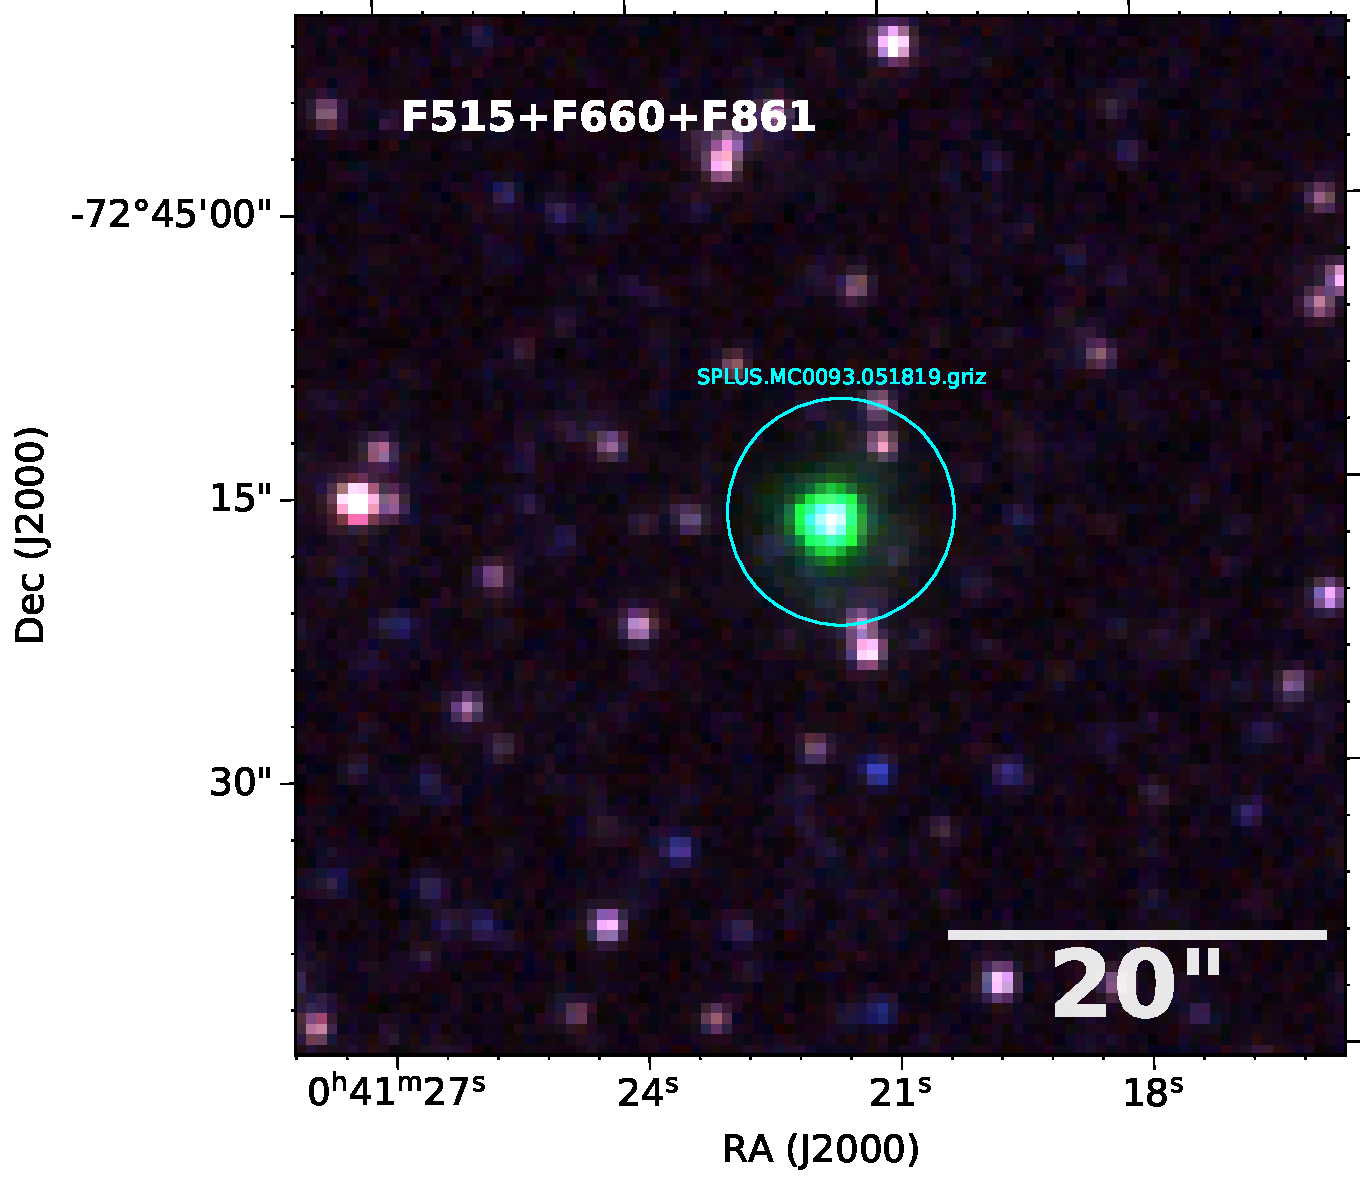
\includegraphics[width=0.3\linewidth, clip]{MC0093/MC0093_F861_051819-RGB.pdf} & 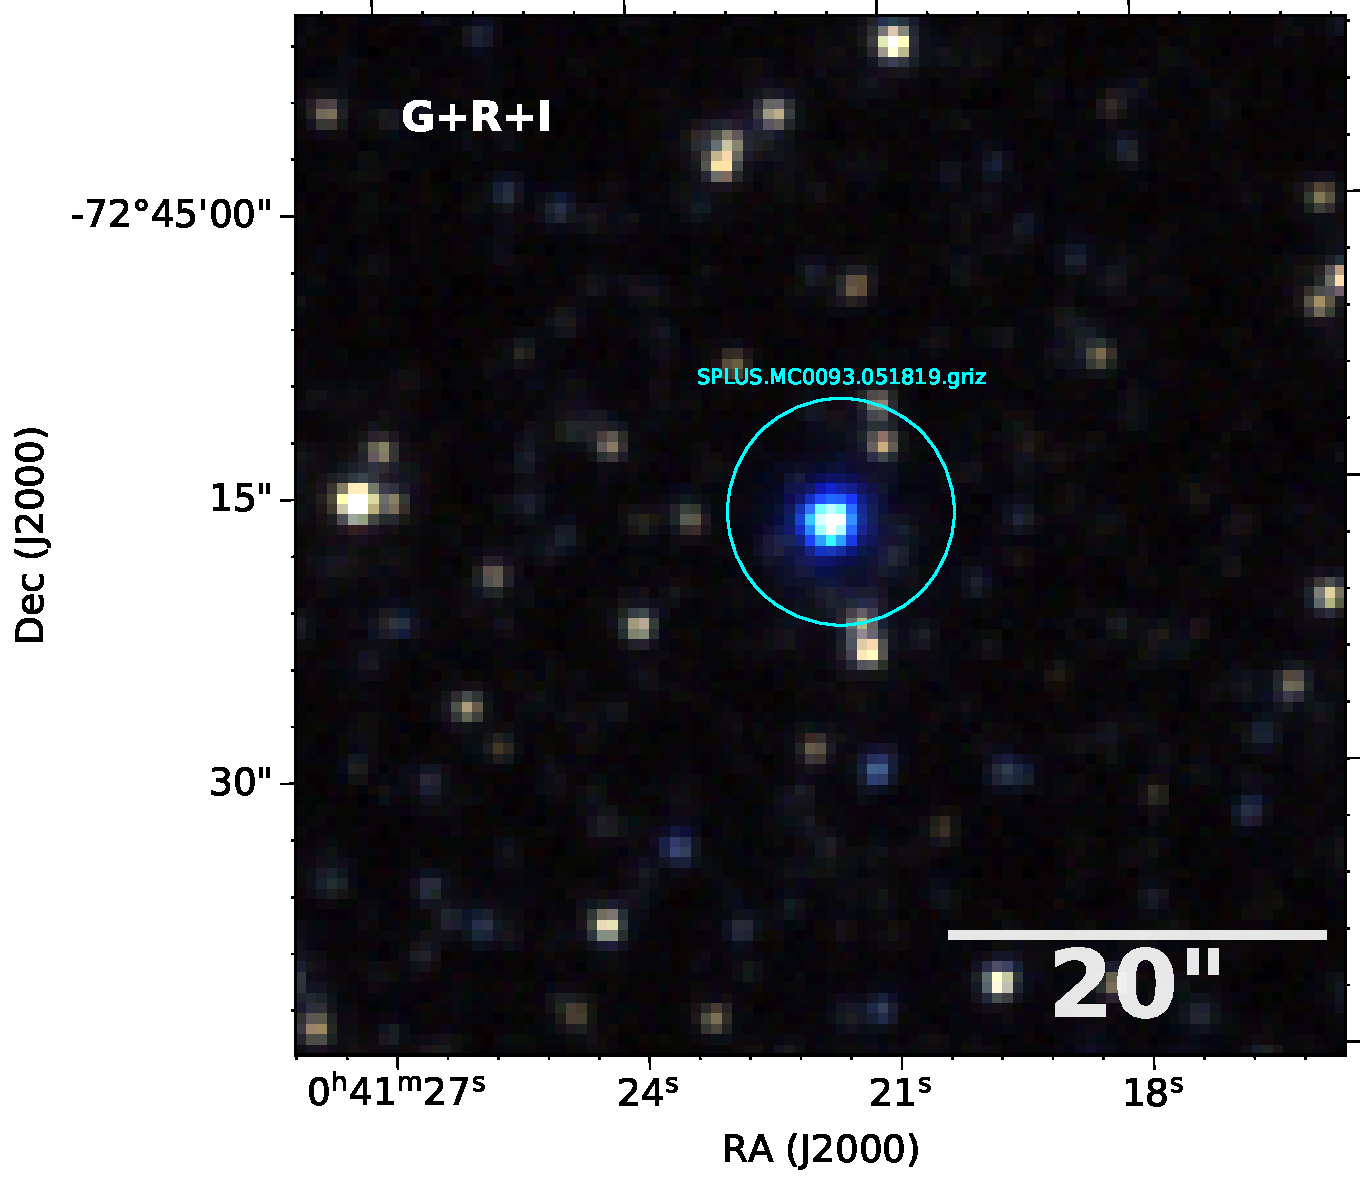
\includegraphics[width=0.3\linewidth, clip]{MC0093/MC0093_I_051819-RGB.pdf} \\
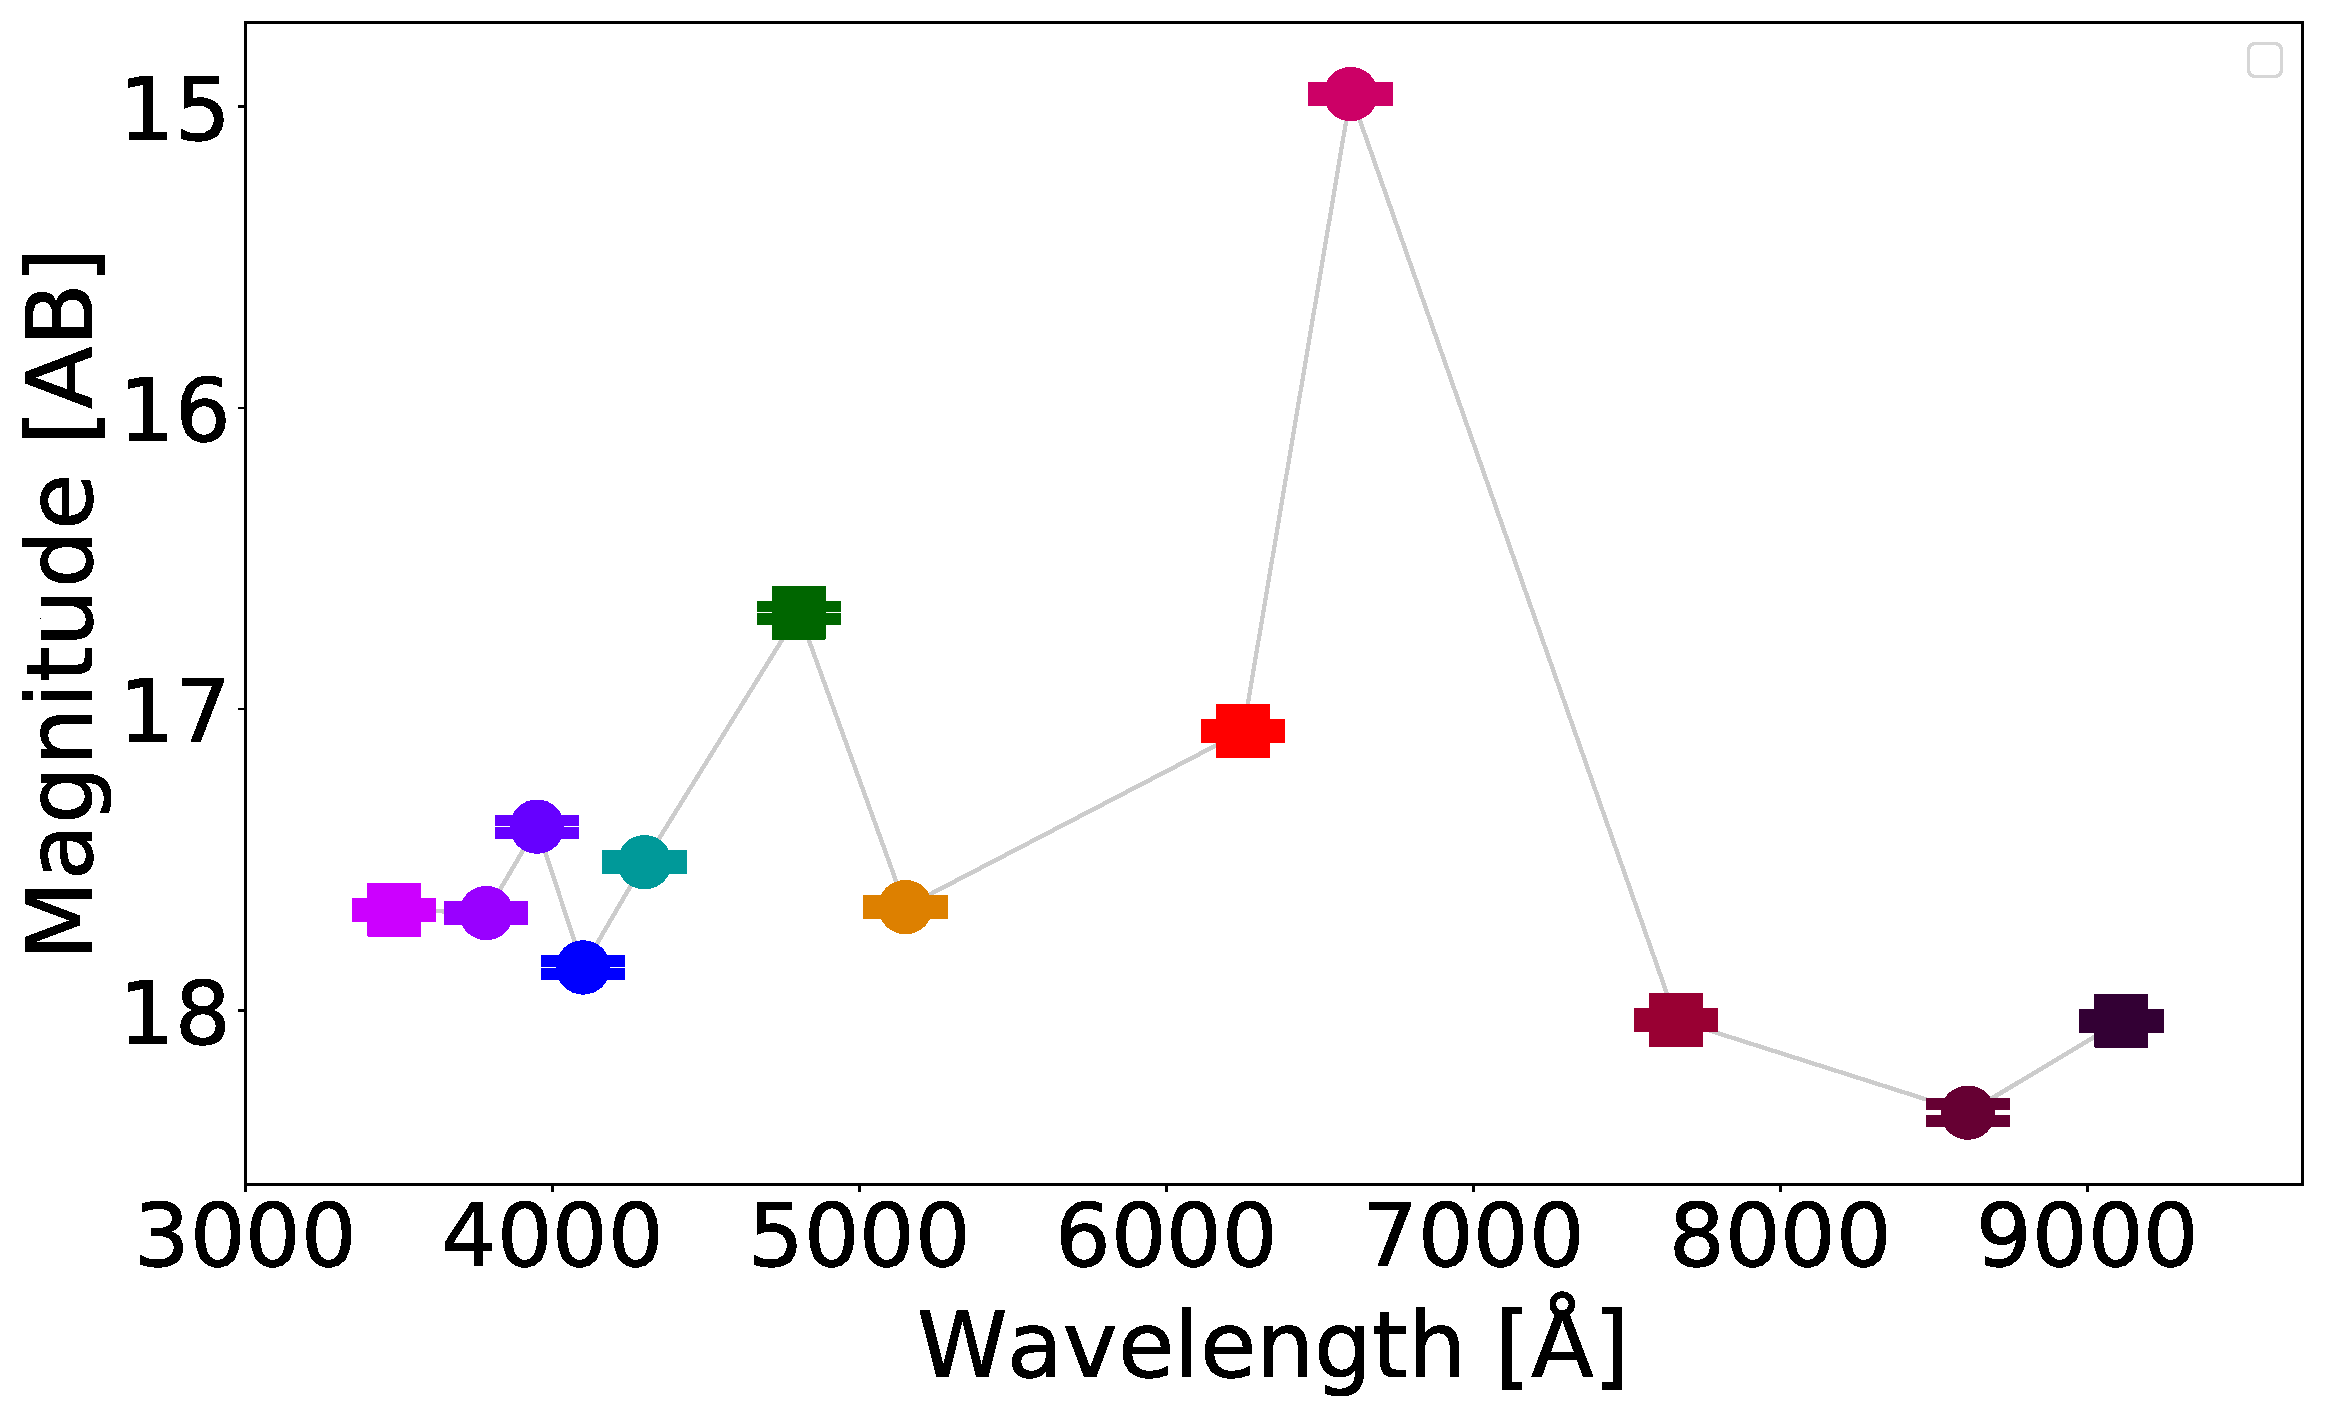
\includegraphics[width=0.3\linewidth, clip]{photopectrum_splus_MC0093-085620_aper.pdf} & 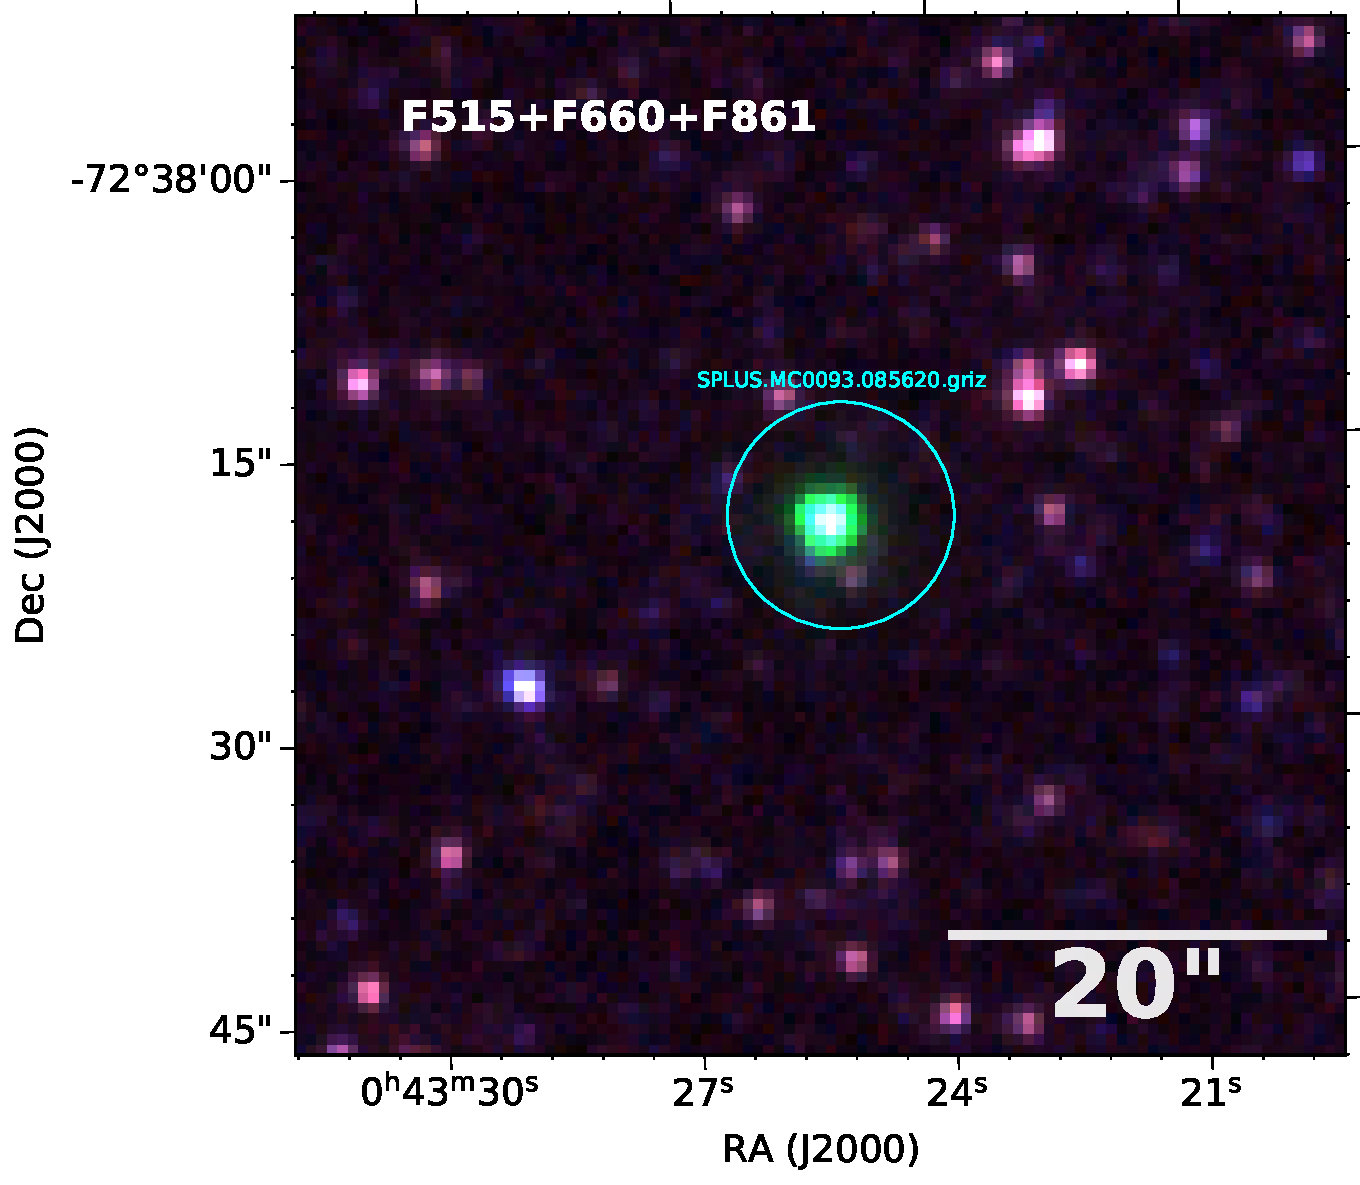
\includegraphics[width=0.3\linewidth, clip]{MC0093/MC0093_F861_085620-RGB.pdf} & 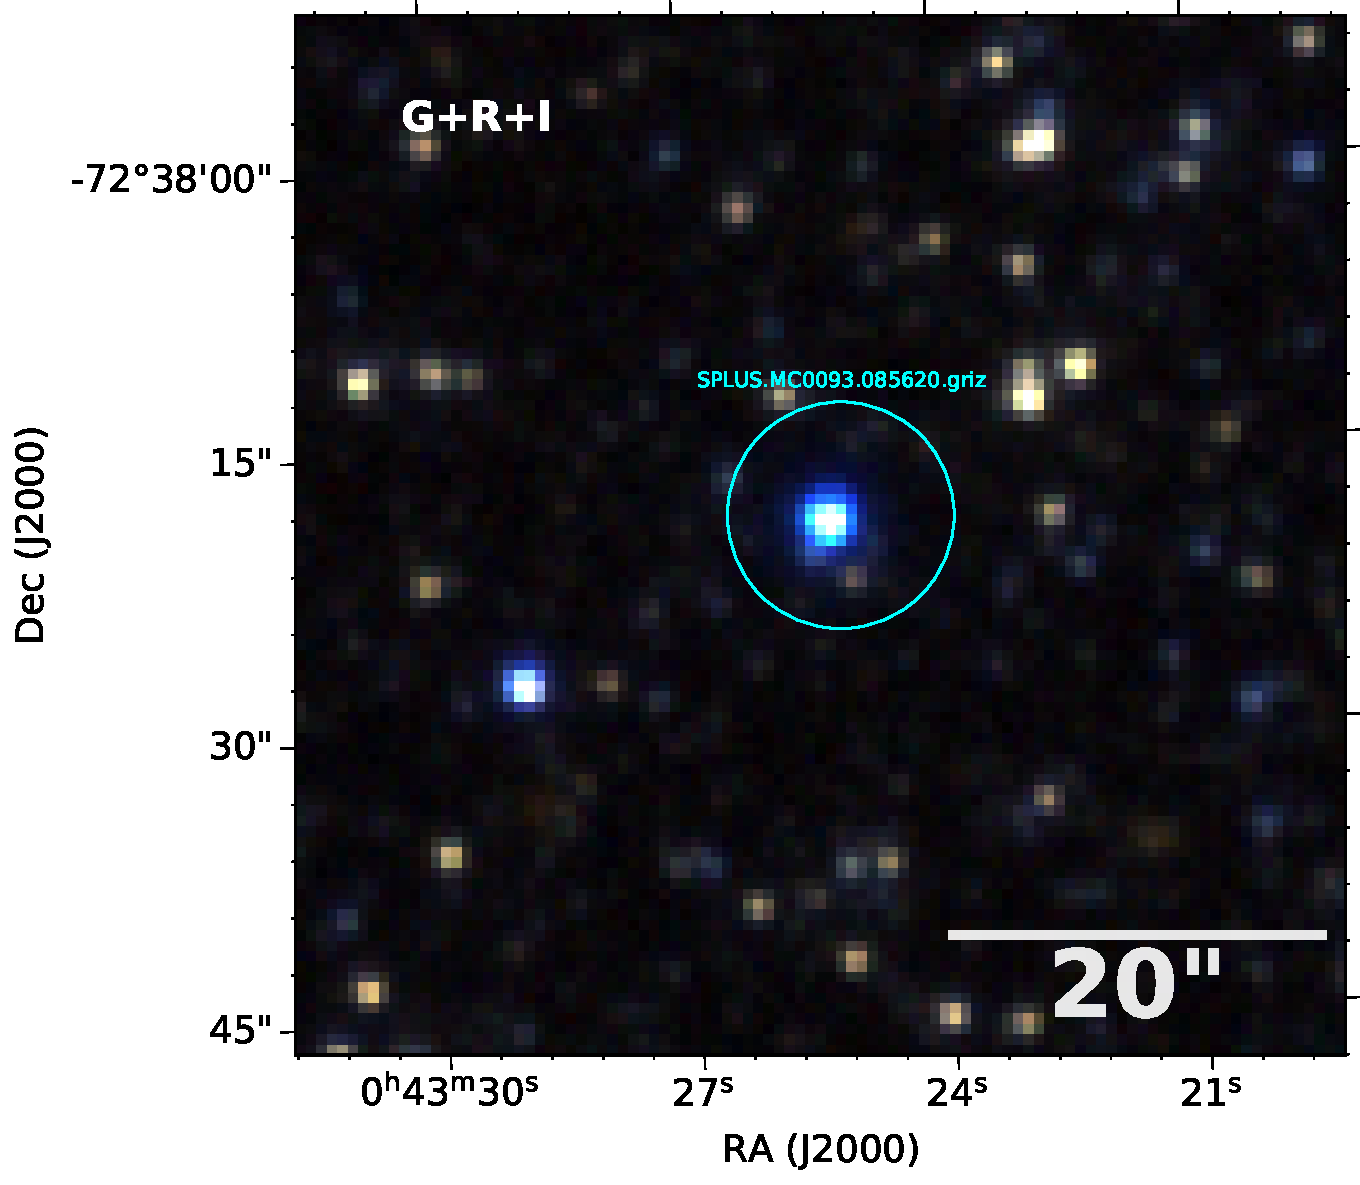
\includegraphics[width=0.3\linewidth, clip]{MC0093/MC0093_I_085620-RGB.pdf} \\
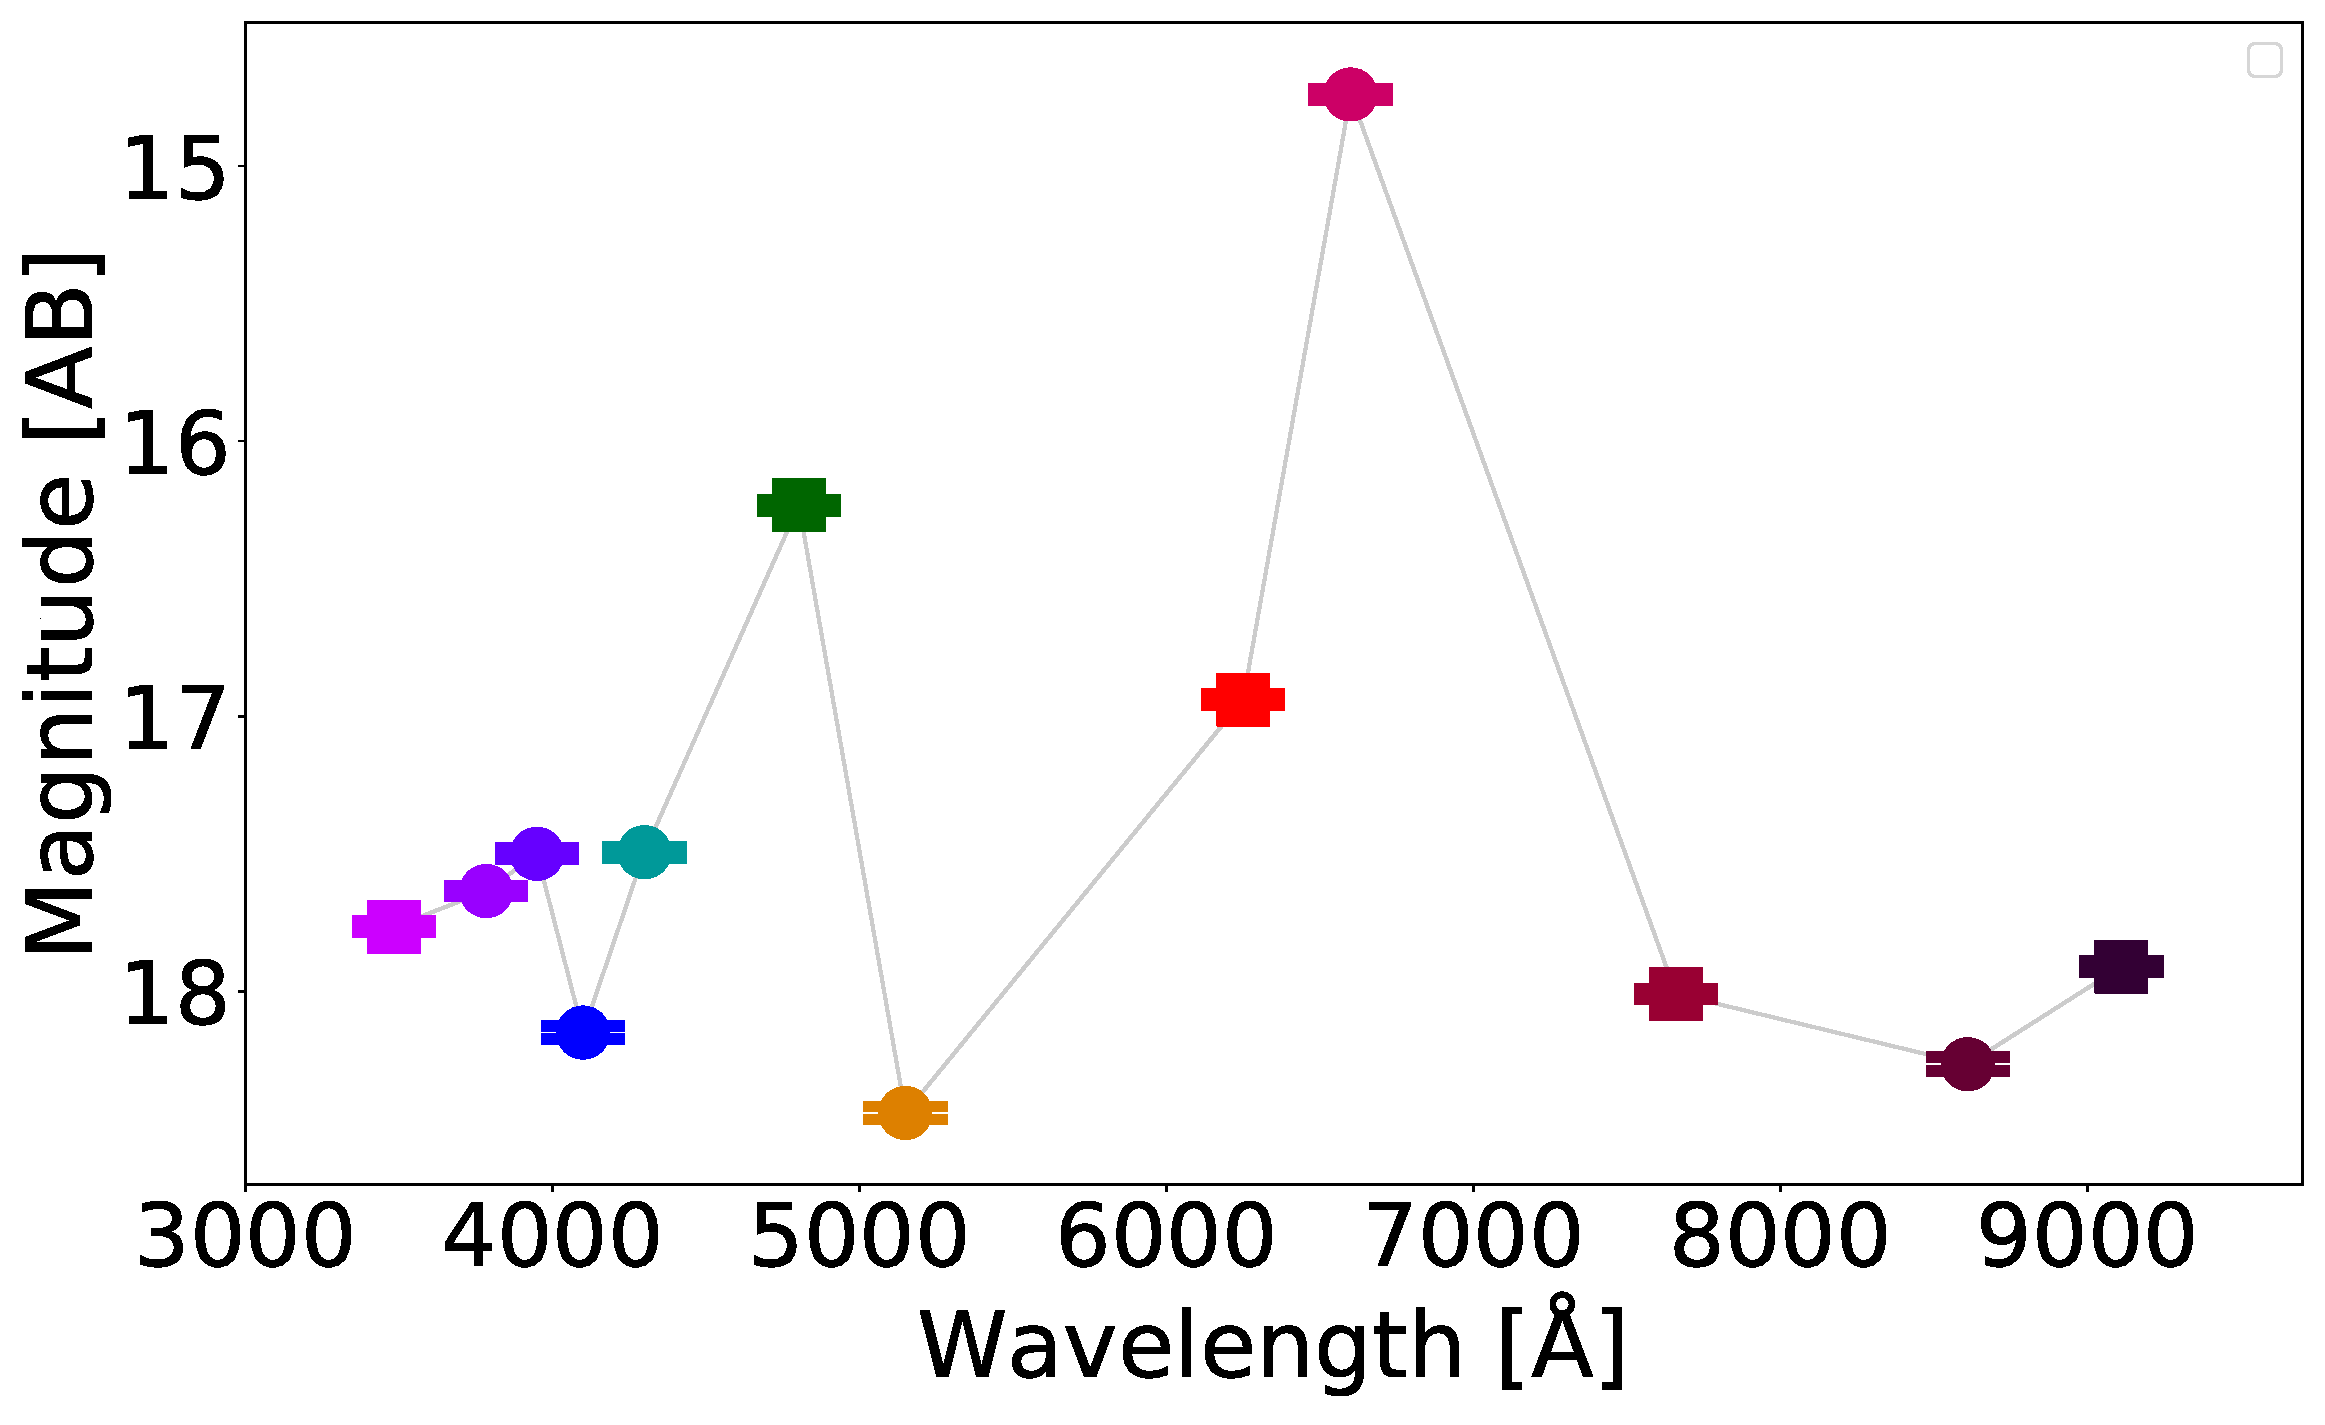
\includegraphics[width=0.3\linewidth, clip]{photopectrum_splus_MC0093-295870_aper.pdf} & \includegraphics[width=0.3\linewidth, clip]{MC0093/MC0093_F861_295870-RGB.pdf} & \includegraphics[width=0.3\linewidth, clip]{MC0093/MC0093_I_295870-RGB.pdf} \\
\includegraphics[width=0.3\linewidth, clip]{photopectrum_splus_MC0094-194143_aper.pdf} & \includegraphics[width=0.3\linewidth, clip]{MC0094/MC0094_F861_194143-RGB.pdf} & \includegraphics[width=0.3\linewidth, clip]{MC0094/MC0094_I_194143-RGB.pdf} \\
\includegraphics[width=0.3\linewidth, clip]{photopectrum_splus_MC0113-084466_aper.pdf} & \includegraphics[width=0.3\linewidth, clip]{MC0113/MC0113_F861_084466-RGB.pdf} & \includegraphics[width=0.3\linewidth, clip]{MC0113/MC0113_I_084466-RGB.pdf} \\
\includegraphics[width=0.3\linewidth, clip]{photopectrum_splus_MC0114-113862_aper.pdf} & \includegraphics[width=0.3\linewidth, clip]{MC0114/MC0114_F861_113862-RGB.pdf} & \includegraphics[width=0.3\linewidth, clip]{MC0114/MC0114_I_113862-RGB.pdf} \\
\includegraphics[width=0.3\linewidth, clip]{photopectrum_splus_MC0114-273678_aper.pdf} & \includegraphics[width=0.3\linewidth, clip]{MC0114/MC0114_F861_273678-RGB.pdf} & \includegraphics[width=0.3\linewidth, clip]{MC0114/MC0114_I_273678-RGB.pdf} \\
\includegraphics[width=0.3\linewidth, clip]{photopectrum_splus_MC0115-043944_aper.pdf} & \includegraphics[width=0.3\linewidth, clip]{MC0115/MC0115_F861_043944-RGB.pdf} & \includegraphics[width=0.3\linewidth, clip]{MC0115/MC0115_I_043944-RGB.pdf} \\
\includegraphics[width=0.3\linewidth, clip]{photopectrum_splus_MC0115-063029_aper.pdf} & \includegraphics[width=0.3\linewidth, clip]{MC0115/MC0115_F861_063029-RGB.pdf} & \includegraphics[width=0.3\linewidth, clip]{MC0115/MC0115_I_063029-RGB.pdf} \\
\includegraphics[width=0.3\linewidth, clip]{photopectrum_splus_MC0115-105523_aper.pdf} & \includegraphics[width=0.3\linewidth, clip]{MC0115/MC0115_F861_105523-RGB.pdf} & \includegraphics[width=0.3\linewidth, clip]{MC0115/MC0115_I_105523-RGB.pdf} \\
\includegraphics[width=0.3\linewidth, clip]{photopectrum_splus_MC0115-112627_aper.pdf} & \includegraphics[width=0.3\linewidth, clip]{MC0115/MC0115_F861_112627-RGB.pdf} & \includegraphics[width=0.3\linewidth, clip]{MC0115/MC0115_I_112627-RGB.pdf} \\
\includegraphics[width=0.3\linewidth, clip]{photopectrum_splus_MC0115-147165_aper.pdf} & \includegraphics[width=0.3\linewidth, clip]{MC0115/MC0115_F861_147165-RGB.pdf} & \includegraphics[width=0.3\linewidth, clip]{MC0115/MC0115_I_147165-RGB.pdf} \\
\includegraphics[width=0.3\linewidth, clip]{photopectrum_splus_MC0115-229578_aper.pdf} & \includegraphics[width=0.3\linewidth, clip]{MC0115/MC0115_F861_229578-RGB.pdf} & \includegraphics[width=0.3\linewidth, clip]{MC0115/MC0115_I_229578-RGB.pdf} \\
\includegraphics[width=0.3\linewidth, clip]{photopectrum_splus_MC0115-308119_aper.pdf} & \includegraphics[width=0.3\linewidth, clip]{MC0115/MC0115_F861_308119-RGB.pdf} & \includegraphics[width=0.3\linewidth, clip]{MC0115/MC0115_I_308119-RGB.pdf} \\
\includegraphics[width=0.3\linewidth, clip]{photopectrum_splus_MC0115-350934_aper.pdf} & \includegraphics[width=0.3\linewidth, clip]{MC0115/MC0115_F861_350934-RGB.pdf} & \includegraphics[width=0.3\linewidth, clip]{MC0115/MC0115_I_350934-RGB.pdf} \\
\includegraphics[width=0.3\linewidth, clip]{photopectrum_splus_MC0115-402039_aper.pdf} & \includegraphics[width=0.3\linewidth, clip]{MC0115/MC0115_F861_402039-RGB.pdf} & \includegraphics[width=0.3\linewidth, clip]{MC0115/MC0115_I_402039-RGB.pdf} \\
\includegraphics[width=0.3\linewidth, clip]{photopectrum_splus_MC0116-015280_aper.pdf} & \includegraphics[width=0.3\linewidth, clip]{MC0116/MC0116_F861_015280-RGB.pdf} & \includegraphics[width=0.3\linewidth, clip]{MC0116/MC0116_I_015280-RGB.pdf} \\
\includegraphics[width=0.3\linewidth, clip]{photopectrum_splus_MC0116-172101_aper.pdf} & \includegraphics[width=0.3\linewidth, clip]{MC0116/MC0116_F861_172101-RGB.pdf} & \includegraphics[width=0.3\linewidth, clip]{MC0116/MC0116_I_172101-RGB.pdf} \\
\includegraphics[width=0.3\linewidth, clip]{photopectrum_splus_MC0133-025038_aper.pdf} & \includegraphics[width=0.3\linewidth, clip]{MC0133/MC0133_F861_025038-RGB.pdf} & \includegraphics[width=0.3\linewidth, clip]{MC0133/MC0133_I_025038-RGB.pdf} \\
%\end{tabular}
%\end{table}


% \end{longtable}
% \end{center}

\newpage
\begin{longtable}{ccc}
  %\caption{Distancias, tamaños y formas de los choques de proa en la Nebulosa de Orión. Las unidades de la distancia y los radios están en [arcsec]. \label{tab:test}}\\

  %\caption[]{continuación }\\
  %\begin{table}
%\begin{tabular}{ccc}
\textbf{Aper(3'')} & \textbf{F515+F660+F861} & \textbf{G+R+I} \\
\includegraphics[width=0.3\linewidth, clip]{photopectrum_splus_MC0072-006125_aper.pdf} & \includegraphics[width=0.3\linewidth, clip]{MC0072/MC0072_F861_006125-RGB.pdf} & \includegraphics[width=0.3\linewidth, clip]{MC0072/MC0072_I_006125-RGB.pdf} \\
\includegraphics[width=0.3\linewidth, clip]{photopectrum_splus_MC0072-044863_aper.pdf} & \includegraphics[width=0.3\linewidth, clip]{MC0072/MC0072_F861_044863-RGB.pdf} & \includegraphics[width=0.3\linewidth, clip]{MC0072/MC0072_I_044863-RGB.pdf} \\
\includegraphics[width=0.3\linewidth, clip]{photopectrum_splus_MC0093-051819_aper.pdf} & \includegraphics[width=0.3\linewidth, clip]{MC0093/MC0093_F861_051819-RGB.pdf} & \includegraphics[width=0.3\linewidth, clip]{MC0093/MC0093_I_051819-RGB.pdf} \\
\includegraphics[width=0.3\linewidth, clip]{photopectrum_splus_MC0093-085620_aper.pdf} & \includegraphics[width=0.3\linewidth, clip]{MC0093/MC0093_F861_085620-RGB.pdf} & \includegraphics[width=0.3\linewidth, clip]{MC0093/MC0093_I_085620-RGB.pdf} \\
\includegraphics[width=0.3\linewidth, clip]{photopectrum_splus_MC0093-295870_aper.pdf} & \includegraphics[width=0.3\linewidth, clip]{MC0093/MC0093_F861_295870-RGB.pdf} & \includegraphics[width=0.3\linewidth, clip]{MC0093/MC0093_I_295870-RGB.pdf} \\
\includegraphics[width=0.3\linewidth, clip]{photopectrum_splus_MC0094-194143_aper.pdf} & \includegraphics[width=0.3\linewidth, clip]{MC0094/MC0094_F861_194143-RGB.pdf} & \includegraphics[width=0.3\linewidth, clip]{MC0094/MC0094_I_194143-RGB.pdf} \\
\includegraphics[width=0.3\linewidth, clip]{photopectrum_splus_MC0113-084466_aper.pdf} & \includegraphics[width=0.3\linewidth, clip]{MC0113/MC0113_F861_084466-RGB.pdf} & \includegraphics[width=0.3\linewidth, clip]{MC0113/MC0113_I_084466-RGB.pdf} \\
\includegraphics[width=0.3\linewidth, clip]{photopectrum_splus_MC0114-113862_aper.pdf} & \includegraphics[width=0.3\linewidth, clip]{MC0114/MC0114_F861_113862-RGB.pdf} & \includegraphics[width=0.3\linewidth, clip]{MC0114/MC0114_I_113862-RGB.pdf} \\
\includegraphics[width=0.3\linewidth, clip]{photopectrum_splus_MC0114-273678_aper.pdf} & \includegraphics[width=0.3\linewidth, clip]{MC0114/MC0114_F861_273678-RGB.pdf} & \includegraphics[width=0.3\linewidth, clip]{MC0114/MC0114_I_273678-RGB.pdf} \\
\includegraphics[width=0.3\linewidth, clip]{photopectrum_splus_MC0115-043944_aper.pdf} & \includegraphics[width=0.3\linewidth, clip]{MC0115/MC0115_F861_043944-RGB.pdf} & \includegraphics[width=0.3\linewidth, clip]{MC0115/MC0115_I_043944-RGB.pdf} \\
\includegraphics[width=0.3\linewidth, clip]{photopectrum_splus_MC0115-063029_aper.pdf} & \includegraphics[width=0.3\linewidth, clip]{MC0115/MC0115_F861_063029-RGB.pdf} & \includegraphics[width=0.3\linewidth, clip]{MC0115/MC0115_I_063029-RGB.pdf} \\
\includegraphics[width=0.3\linewidth, clip]{photopectrum_splus_MC0115-105523_aper.pdf} & \includegraphics[width=0.3\linewidth, clip]{MC0115/MC0115_F861_105523-RGB.pdf} & \includegraphics[width=0.3\linewidth, clip]{MC0115/MC0115_I_105523-RGB.pdf} \\
\includegraphics[width=0.3\linewidth, clip]{photopectrum_splus_MC0115-112627_aper.pdf} & \includegraphics[width=0.3\linewidth, clip]{MC0115/MC0115_F861_112627-RGB.pdf} & \includegraphics[width=0.3\linewidth, clip]{MC0115/MC0115_I_112627-RGB.pdf} \\
\includegraphics[width=0.3\linewidth, clip]{photopectrum_splus_MC0115-147165_aper.pdf} & \includegraphics[width=0.3\linewidth, clip]{MC0115/MC0115_F861_147165-RGB.pdf} & \includegraphics[width=0.3\linewidth, clip]{MC0115/MC0115_I_147165-RGB.pdf} \\
\includegraphics[width=0.3\linewidth, clip]{photopectrum_splus_MC0115-229578_aper.pdf} & \includegraphics[width=0.3\linewidth, clip]{MC0115/MC0115_F861_229578-RGB.pdf} & \includegraphics[width=0.3\linewidth, clip]{MC0115/MC0115_I_229578-RGB.pdf} \\
\includegraphics[width=0.3\linewidth, clip]{photopectrum_splus_MC0115-308119_aper.pdf} & \includegraphics[width=0.3\linewidth, clip]{MC0115/MC0115_F861_308119-RGB.pdf} & \includegraphics[width=0.3\linewidth, clip]{MC0115/MC0115_I_308119-RGB.pdf} \\
\includegraphics[width=0.3\linewidth, clip]{photopectrum_splus_MC0115-350934_aper.pdf} & \includegraphics[width=0.3\linewidth, clip]{MC0115/MC0115_F861_350934-RGB.pdf} & \includegraphics[width=0.3\linewidth, clip]{MC0115/MC0115_I_350934-RGB.pdf} \\
\includegraphics[width=0.3\linewidth, clip]{photopectrum_splus_MC0115-402039_aper.pdf} & \includegraphics[width=0.3\linewidth, clip]{MC0115/MC0115_F861_402039-RGB.pdf} & \includegraphics[width=0.3\linewidth, clip]{MC0115/MC0115_I_402039-RGB.pdf} \\
\includegraphics[width=0.3\linewidth, clip]{photopectrum_splus_MC0116-015280_aper.pdf} & \includegraphics[width=0.3\linewidth, clip]{MC0116/MC0116_F861_015280-RGB.pdf} & \includegraphics[width=0.3\linewidth, clip]{MC0116/MC0116_I_015280-RGB.pdf} \\
\includegraphics[width=0.3\linewidth, clip]{photopectrum_splus_MC0116-172101_aper.pdf} & \includegraphics[width=0.3\linewidth, clip]{MC0116/MC0116_F861_172101-RGB.pdf} & \includegraphics[width=0.3\linewidth, clip]{MC0116/MC0116_I_172101-RGB.pdf} \\
\includegraphics[width=0.3\linewidth, clip]{photopectrum_splus_MC0133-025038_aper.pdf} & \includegraphics[width=0.3\linewidth, clip]{MC0133/MC0133_F861_025038-RGB.pdf} & \includegraphics[width=0.3\linewidth, clip]{MC0133/MC0133_I_025038-RGB.pdf} \\
%\end{tabular}
%\end{table}

\end{longtable}

\subsection{What about compact H II regions}
\label{sec:ini}

I found a catalog of 12 compact H II regions (\url{2012SerAJ.185...53W}) in the SMC SPLUS
   catalog. In Simbad appear reported like emission line stars.

\begin{figure*}
%\setlength\tabcolsep{\figstampcolsep}
\end{figure*}

\begin{figure*}
  \centering
\begin{tabular}{l l}
\includegraphics[width=0.5\linewidth, trim=10 10 10 10, clip]{Fig1-pne-smc-splus-match-2007-compat-HIIRegions-smc-match-splus-vironen.pdf} & \\
 \includegraphics[width=0.5\linewidth, trim=10 10 10 10, clip]{Fig2-pne-smc-splus-match-2007-compat-HIIRegions-smc-match-splus-J0515_J0660.pdf} & \includegraphics[width=0.5\linewidth, trim=10 10 10 10, clip]{Fig4-pne-smc-splus-match-2007-compat-HIIRegions-smc-match-splus-g.pdf} \\
%\raiselabel{(\textit{a})} & \raiselabel{(\textit{b})}\\
\includegraphics[width=0.5\linewidth, trim=10 10 10 10, clip]{Fig3-pne-smc-splus-match-2007-compat-HIIRegions-smc-match-splus-z.pdf} & \includegraphics[width=0.5\linewidth, trim=10 10 10 10, clip]{Fig5-pne-smc-splus-match-2007-compat-HIIRegions-smc-match-splus-gi.pdf} \\
%\raiselabel{(\textit{c})} & \raiselabel{(\textit{d})}
\end{tabular}
\caption{}
\label{fig:smppne}
\end{figure*}
  
\newpage
\begin{longtable}{ccc}
  %\caption[]{continuación }\\
  % \begin{table}
% \begin{tabular}{ccc}
\textbf{Aper (3'')} & \textbf{Auto} & \textbf{Petro} \\
\includegraphics[width=0.3\linewidth, clip]{photopectrum_splus_MC0094-318227_compat-HIIRegions-smc-match-splus_aper.pdf} & \includegraphics[width=0.3\linewidth, clip]{photopectrum_splus_MC0094-318227_compat-HIIRegions-smc-match-splus_auto.pdf} & \includegraphics[width=0.3\linewidth, clip]{photopectrum_splus_MC0094-318227_compat-HIIRegions-smc-match-splus_petro.pdf} \\
\includegraphics[width=0.3\linewidth, clip]{photopectrum_splus_MC0095-257970_compat-HIIRegions-smc-match-splus_aper.pdf} & \includegraphics[width=0.3\linewidth, clip]{photopectrum_splus_MC0095-257970_compat-HIIRegions-smc-match-splus_auto.pdf} & \includegraphics[width=0.3\linewidth, clip]{photopectrum_splus_MC0095-257970_compat-HIIRegions-smc-match-splus_petro.pdf} \\
\includegraphics[width=0.3\linewidth, clip]{photopectrum_splus_MC0095-265990_compat-HIIRegions-smc-match-splus_aper.pdf} & \includegraphics[width=0.3\linewidth, clip]{photopectrum_splus_MC0095-265990_compat-HIIRegions-smc-match-splus_auto.pdf} & \includegraphics[width=0.3\linewidth, clip]{photopectrum_splus_MC0095-265990_compat-HIIRegions-smc-match-splus_petro.pdf} \\
\includegraphics[width=0.3\linewidth, clip]{photopectrum_splus_MC0114-222322_compat-HIIRegions-smc-match-splus_aper.pdf} & \includegraphics[width=0.3\linewidth, clip]{photopectrum_splus_MC0114-222322_compat-HIIRegions-smc-match-splus_auto.pdf} & \includegraphics[width=0.3\linewidth, clip]{photopectrum_splus_MC0114-222322_compat-HIIRegions-smc-match-splus_petro.pdf} \\
\includegraphics[width=0.3\linewidth, clip]{photopectrum_splus_MC0114-327430_compat-HIIRegions-smc-match-splus_aper.pdf} & \includegraphics[width=0.3\linewidth, clip]{photopectrum_splus_MC0114-327430_compat-HIIRegions-smc-match-splus_auto.pdf} & \includegraphics[width=0.3\linewidth, clip]{photopectrum_splus_MC0114-327430_compat-HIIRegions-smc-match-splus_petro.pdf} \\
\includegraphics[width=0.3\linewidth, clip]{photopectrum_splus_MC0115-152415_compat-HIIRegions-smc-match-splus_aper.pdf} & \includegraphics[width=0.3\linewidth, clip]{photopectrum_splus_MC0115-152415_compat-HIIRegions-smc-match-splus_auto.pdf} & \includegraphics[width=0.3\linewidth, clip]{photopectrum_splus_MC0115-152415_compat-HIIRegions-smc-match-splus_petro.pdf} \\
\includegraphics[width=0.3\linewidth, clip]{photopectrum_splus_MC0115-287587_compat-HIIRegions-smc-match-splus_aper.pdf} & \includegraphics[width=0.3\linewidth, clip]{photopectrum_splus_MC0115-287587_compat-HIIRegions-smc-match-splus_auto.pdf} & \includegraphics[width=0.3\linewidth, clip]{photopectrum_splus_MC0115-287587_compat-HIIRegions-smc-match-splus_petro.pdf} \\
\includegraphics[width=0.3\linewidth, clip]{photopectrum_splus_MC0115-397126_compat-HIIRegions-smc-match-splus_aper.pdf} & \includegraphics[width=0.3\linewidth, clip]{photopectrum_splus_MC0115-397126_compat-HIIRegions-smc-match-splus_auto.pdf} & \includegraphics[width=0.3\linewidth, clip]{photopectrum_splus_MC0115-397126_compat-HIIRegions-smc-match-splus_petro.pdf} \\
\includegraphics[width=0.3\linewidth, clip]{photopectrum_splus_MC0116-158507_compat-HIIRegions-smc-match-splus_aper.pdf} & \includegraphics[width=0.3\linewidth, clip]{photopectrum_splus_MC0116-158507_compat-HIIRegions-smc-match-splus_auto.pdf} & \includegraphics[width=0.3\linewidth, clip]{photopectrum_splus_MC0116-158507_compat-HIIRegions-smc-match-splus_petro.pdf} \\
\includegraphics[width=0.3\linewidth, clip]{photopectrum_splus_MC0116-168236_compat-HIIRegions-smc-match-splus_aper.pdf} & \includegraphics[width=0.3\linewidth, clip]{photopectrum_splus_MC0116-168236_compat-HIIRegions-smc-match-splus_auto.pdf} & \includegraphics[width=0.3\linewidth, clip]{photopectrum_splus_MC0116-168236_compat-HIIRegions-smc-match-splus_petro.pdf} \\
\includegraphics[width=0.3\linewidth, clip]{photopectrum_splus_MC0116-170015_compat-HIIRegions-smc-match-splus_aper.pdf} & \includegraphics[width=0.3\linewidth, clip]{photopectrum_splus_MC0116-170015_compat-HIIRegions-smc-match-splus_auto.pdf} & \includegraphics[width=0.3\linewidth, clip]{photopectrum_splus_MC0116-170015_compat-HIIRegions-smc-match-splus_petro.pdf} \\
\includegraphics[width=0.3\linewidth, clip]{photopectrum_splus_MC0116-191358_compat-HIIRegions-smc-match-splus_aper.pdf} & \includegraphics[width=0.3\linewidth, clip]{photopectrum_splus_MC0116-191358_compat-HIIRegions-smc-match-splus_auto.pdf} & \includegraphics[width=0.3\linewidth, clip]{photopectrum_splus_MC0116-191358_compat-HIIRegions-smc-match-splus_petro.pdf} \\
% \end{tabular}
% \end{table}

\end{longtable} 

\newpage
\begin{figure*}[!h]
% %\setlength\tabcolsep{\figstampcolsep}
\centering
\begin{tabular}{ccc}
\textbf{Aper(3'')} & \textbf{F515+F660+F861} & \textbf{G+R+I} \\
\includegraphics[width=0.3\linewidth, clip]{photopectrum_splus_MC0094-318227_compat-HIIRegions-smc-match-splus_aper.pdf} & \includegraphics[width=0.3\linewidth, clip]{MC0094/MC0094_F861_318227-RGB-hii.pdf} & \includegraphics[width=0.3\linewidth, clip]{MC0094/MC0094_I_318227-RGB-hii.pdf} \\
\includegraphics[width=0.3\linewidth, clip]{photopectrum_splus_MC0095-257970_compat-HIIRegions-smc-match-splus_aper.pdf} & \includegraphics[width=0.3\linewidth, clip]{MC0095/MC0095_F861_257970-RGB-hii.pdf} & \includegraphics[width=0.3\linewidth, clip]{MC0095/MC0095_I_257970-RGB-hii.pdf} \\
\includegraphics[width=0.3\linewidth, clip]{photopectrum_splus_MC0095-265990_compat-HIIRegions-smc-match-splus_aper.pdf} & \includegraphics[width=0.3\linewidth, clip]{MC0095/MC0095_F861_265990-RGB-hii.pdf} & \includegraphics[width=0.3\linewidth, clip]{MC0095/MC0095_I_265990-RGB-hii.pdf} \\
\includegraphics[width=0.3\linewidth, clip]{photopectrum_splus_MC0114-222322_compat-HIIRegions-smc-match-splus_aper.pdf} & \includegraphics[width=0.3\linewidth, clip]{MC0114/MC0114_F861_222322-RGB-hii.pdf} & \includegraphics[width=0.3\linewidth, clip]{MC0114/MC0114_I_222322-RGB-hii.pdf} \\
\includegraphics[width=0.3\linewidth, clip]{photopectrum_splus_MC0116-191358_compat-HIIRegions-smc-match-splus_aper.pdf} & \includegraphics[width=0.3\linewidth, clip]{MC0116/MC0116_F861_191358-RGB-hii.pdf} & \includegraphics[width=0.3\linewidth, clip]{MC0116/MC0116_I_191358-RGB-hii.pdf} \\
% \includegraphics[width=0.3\linewidth, clip]{photopectrum_splus_MC0094-194143_aper.pdf} & \includegraphics[width=0.3\linewidth, clip]{MC0094/MC0094_F861_194143-RGB.pdf} & \includegraphics[width=0.3\linewidth, clip]{MC0094/MC0094_I_194143-RGB.pdf} \\
% \includegraphics[width=0.3\linewidth, clip]{photopectrum_splus_MC0113-084466_aper.pdf} & \includegraphics[width=0.3\linewidth, clip]{MC0113/MC0113_F861_084466-RGB.pdf} & \includegraphics[width=0.3\linewidth, clip]{MC0113/MC0113_I_084466-RGB.pdf} \\
% \includegraphics[width=0.3\linewidth, clip]{photopectrum_splus_MC0114-113862_aper.pdf} & \includegraphics[width=0.3\linewidth, clip]{MC0114/MC0114_F861_113862-RGB.pdf} & \includegraphics[width=0.3\linewidth, clip]{MC0114/MC0114_I_113862-RGB.pdf} \\
% \includegraphics[width=0.3\linewidth, clip]{photopectrum_splus_MC0114-273678_aper.pdf} & \includegraphics[width=0.3\linewidth, clip]{MC0114/MC0114_F861_273678-RGB.pdf} & \includegraphics[width=0.3\linewidth, clip]{MC0114/MC0114_I_273678-RGB.pdf} \\
 \end{tabular}
\caption{}
\end{figure*}

\newpage
\subsubsection{Comparing SPLUS images with HST}
\label{sec:hst}
The professor Denise found HST information for four of these objects. She sent me the information that follows (I added the SPLUS imges).

A import detail about the paper cited in below document. "The nebular diameters, given in column (5), were measured with respect to the 10\% intensity contour of the outermost structure and are useful for conducting follow-on observations of the PNe." And the paper (\url{2003ApJ...596..997S}) used the same method to measured the size. "the nebular dimensions, measured from the 10\% brightness contour".

\includepdf[page=-]{HSTimages-sizes_SMCPNe.pdf}

\end{document}
